\documentclass[12pt,a4paper]{report}

% ---------- Page geometry ----------
\usepackage[a4paper,margin=2.5cm]{geometry}
\usepackage{setspace}
\onehalfspacing

% ---------- Fonts ----------
\usepackage[T1]{fontenc}
\usepackage{newtxtext,newtxmath} % Times-like

% ---------- Core packages ----------
\usepackage{microtype} % font expansion/protrusion: reduces overfull/underfull hbox warnings
\usepackage{graphicx}
\usepackage{booktabs}
\usepackage{longtable}
\usepackage{array}
\usepackage{caption}
\usepackage{subcaption}
\usepackage{amsmath}
\usepackage{listings}
\usepackage{xcolor}
\usepackage{titlesec}
\usepackage{tocloft}
\usepackage{fancyhdr}
\usepackage[hidelinks]{hyperref}
\usepackage{xurl} % allow URLs (in references) to break at any character, avoiding overfull hboxes
\usepackage{enumitem}
\usepackage{float}
\usepackage{rotating}
\usepackage{pdflscape}

% ---------- Page numbering bottom centre ----------
\pagestyle{plain}
\fancyhf{}
\fancyfoot[C]{\thepage}
\renewcommand{\headrulewidth}{0pt}
\pagestyle{fancy}

% ---------- Chapter / section heading style (centred CHAPTER N) ----------
\titleformat{\chapter}[display]
  {\centering\bfseries}
  {\MakeUppercase{\chaptertitlename} \thechapter}
  {4pt}
  {\centering\MakeUppercase}
\titlespacing*{\chapter}{0pt}{0pt}{18pt}

\titleformat{\section}
  {\bfseries\large}{\thesection}{1em}{}
\titleformat{\subsection}
  {\bfseries\normalsize}{\thesubsection}{1em}{}

% ---------- Captions ----------
\captionsetup[figure]{labelfont=bf,font=small,name=Figure,skip=4pt}
\captionsetup[table]{labelfont=bf,font=small,name=Table,skip=4pt}

% ---------- Tighter float spacing (reduces page count with many figures) ----------
\setlength{\textfloatsep}{8pt plus 1pt minus 2pt}
\setlength{\intextsep}{6pt plus 1pt minus 1pt}
\setlength{\floatsep}{6pt plus 1pt minus 1pt}

% ---------- Listings ----------
\definecolor{codegray}{rgb}{0.95,0.95,0.95}
\lstset{
  basicstyle=\ttfamily\scriptsize,
  backgroundcolor=\color{codegray},
  frame=single,
  numbers=left,
  numberstyle=\tiny\color{gray},
  breaklines=true,
  breakatwhitespace=false,
  showstringspaces=false,
  columns=flexible,
  keepspaces=true,
  captionpos=b,
  tabsize=2,
  aboveskip=4pt,
  belowskip=4pt,
}

% ---------- Compact (single) spacing inside listings ----------
% \onehalfspacing above is meant for body prose; applying it inside code
% listings as well makes every listing far longer than necessary.
\AtBeginEnvironment{lstlisting}{\singlespacing}

% ---------- TOC depth ----------
\setcounter{tocdepth}{1}
\setcounter{secnumdepth}{3}

% Allow a line break after every literal underscore (used throughout for
% file paths, config keys, and code identifiers) so long identifiers like
% experimental_design_corrections.md do not overflow the line.
\let\origunderscore\_
\renewcommand{\_}{\origunderscore\allowbreak}

\newcommand{\checkitem}{\textbf{[CHECK]}}
\renewcommand{\cite}[1]{[\ref{#1}]}

\begin{document}

% ================= FRONT MATTER (roman numerals) =================
\pagenumbering{roman}

\begin{titlepage}
\centering
\vspace*{0.5cm}

{\LARGE \bfseries LIVE REINFORCEMENT LEARNING VERSUS\\[2pt] THRESHOLD-BASED AUTOSCALING IN KUBERNETES \par}

\vspace{1.2cm}
{\large \bfseries A CAPSTONE PROJECT REPORT \par}

\vspace{0.8cm}
{\normalsize
Submitted in partial fulfillment of the\\
requirement for the award of the\\
Degree of\par}

\vspace{0.5cm}
{\normalsize \bfseries BACHELOR OF TECHNOLOGY \par}
{\normalsize \bfseries IN \par}
{\normalsize \bfseries COMPUTER SCIENCE AND ENGINEERING \par}

\vspace{0.8cm}
{\normalsize by \par}

\vspace{0.4cm}
{\normalsize \bfseries
DANDAMUDI RAKESH (23BCE7528)\par
KOTAPURI SATHVIK (23BCE20112)\par
RACHUMALLU VISWANADH (23BCE7431)\par
BOTLAGUNTA THOUSHIK (23BCE20327)\par}

\vspace{0.8cm}
{\normalsize Under the Guidance of \par}
\vspace{0.2cm}
{\normalsize \bfseries DR. SHEELA JAYACHANDRAN \par}

\vspace{1.0cm}

\includegraphics[width=3.5cm]{assets/vitap_logo.png}

\vspace{1.0cm}
{\normalsize \bfseries SCHOOL OF COMPUTER SCIENCE AND ENGINEERING \par}
{\normalsize \bfseries VIT-AP UNIVERSITY \par}
{\normalsize \bfseries AMARAVATI- 522237 \par}

\vspace{0.6cm}
{\normalsize \textit{NOVEMBER 2026} \par}

\end{titlepage}

\chapter*{\centering CERTIFICATE}
\addcontentsline{toc}{chapter}{Certificate}

This is to certify that the Capstone Project work titled
\textbf{\textit{``Live Reinforcement Learning Versus Threshold-Based Autoscaling in Kubernetes''}}
that is being submitted by \textbf{DANDAMUDI RAKESH (23BCE7528)},
\textbf{KOTAPURI SATHVIK (23BCE20112)}, \textbf{RACHUMALLU VISWANADH (23BCE7431)}
and \textbf{BOTLAGUNTA THOUSHIK (23BCE20327)} is in partial fulfillment of the
requirements for the award of \textbf{Bachelor of Technology}, is a record of
bonafide work done under my guidance. The contents of this report, in full or
in part, have not been submitted to any other Institute or University for the
award of any degree or diploma.

\vspace{2.0cm}

\begin{flushright}
\textbf{Dr. Sheela Jayachandran} \\
Associate Professor Grade-1 \\
School of Computer Science and Engineering \\
VIT-AP University \\
\textbf{Guide}
\end{flushright}

\vspace{1.5cm}

\begin{center}
The thesis is satisfactory / unsatisfactory
\end{center}

\vspace{1.2cm}

\noindent
\begin{minipage}[t]{0.45\textwidth}
\centering
Internal Examiner
\end{minipage}
\hfill
\begin{minipage}[t]{0.45\textwidth}
\centering
External Examiner
\end{minipage}

\vspace{1.5cm}

\begin{center}
Approved by
\end{center}

\vspace{1.0cm}

\noindent
\begin{minipage}[t]{0.45\textwidth}
\centering
\textbf{PROGRAM CHAIR} \\
B.Tech. CSE
\end{minipage}
\hfill
\begin{minipage}[t]{0.45\textwidth}
\centering
\textbf{DEAN} \\
School of Computer Science and Engineering
\end{minipage}

\chapter*{\centering ACKNOWLEDGEMENTS}
\label{ch:acknowledgements}
\addcontentsline{toc}{chapter}{Acknowledgements}

We would like to thank our guide, Dr. Sheela Jayachandran, Associate
Professor Grade-1, School of Computer Science and Engineering, VIT-AP
University, for the steady direction she gave this project from its first,
much smaller proposal through to the full system described in this report.
Her insistence that every claim be checked against the actual cluster, and
not against what we expected the cluster to do, shaped the project's whole
approach to evidence and is the reason this report can trace every number
back to a file in our repository.

We thank the Dean, School of Computer Science and Engineering, and the
Program Chair, B.Tech. Computer Science and Engineering, for approving this
topic and for the laboratory and infrastructure support that let us run a
live Kubernetes cluster for training and evaluation over several weeks. We
also thank the faculty and staff of the School who reviewed our proposal and
gave feedback at the proposal and mid-term review stages; several of the
checks built into our experimental design, in particular the pre-registration
of the evaluation protocol before any evaluation run, came directly out of
questions raised in those reviews.

This project would not have been possible without the open-source projects it
is built on. We thank the Kubernetes and Minikube projects for a container
orchestration platform and a local single-node cluster that behaves closely
enough to a production cluster to make the comparison in this report
meaningful; the Prometheus and kube-prometheus-stack maintainers for the
telemetry our RL agent and both HPA baselines depend on; the Stable-Baselines3
and Gymnasium maintainers for a well-tested PPO implementation and a standard
environment interface that let us focus on the Kubernetes-specific parts of
the problem rather than re-implementing PPO from scratch; the PyTorch project,
which Stable-Baselines3 is built on; the FastAPI maintainers, whose framework
runs our benchmark service; and the Streamlit, Plotly, Matplotlib, and
Graphviz projects, which we used respectively for our demonstration console
and for the figures and diagrams in this report. Docker and Docker Desktop
made it practical to run all of this on a single laptop.

AI assistants were used to help author code and for language editing; the
experimental design, all experiments, data and conclusions are our own.

Finally, we thank our families for their patience during the weeks this
project's training and evaluation campaigns ran on a laptop that could not be
used for much else while a live cluster was being measured.

\vspace{1.0cm}
\noindent
Dandamudi Rakesh\\
Kotapuri Sathvik\\
Rachumallu Viswanadh\\
Botlagunta Thoushik

\chapter*{\centering ABSTRACT}
\label{ch:abstract}
\addcontentsline{toc}{chapter}{Abstract}

The Kubernetes Horizontal Pod Autoscaler (HPA) resizes a deployment only
after a chosen utilization metric crosses a fixed threshold, and it cannot
use experience from past traffic to anticipate future load. This report
describes a capstone project that trained a Proximal Policy Optimization
(PPO) agent directly against a live, single-node Minikube cluster, with no
simulator standing in for the cluster at any stage, and compared it against
two HPA configurations on traffic none of the controllers had seen before.
The agent observes eleven normalized signals covering CPU, memory, request
rate, and latency, together with their short-horizon trends; its raw action
passes through a deterministic safety layer -- a replica-bound clamp, a
pending-scale gate, and an asymmetric scale-down cooldown -- before it ever
reaches the Kubernetes API, and an uncertain policy is resolved by a
safety-aware tie-break rule that can never let scale-down win a tie. The
agent trained for 12,288 live decision steps across 48 sessions, during
which explained variance of the value function rose from 0.0125 at the
first update to a mean of 0.703 over the last five updates (peaking at
0.799), computed directly from the training campaign's own update log. Two
of the 48 planned sessions stopped early when every ready replica of the
deployment briefly dropped to zero under correlated pod unhealthiness; both
resumed from their last checkpoint and completed successfully, and we
report this as a genuine property of running training against a real
cluster rather than omitting it. We then ran a pre-registered, 27-run
held-out evaluation of this policy against an HPA configuration using CPU
and memory and a CPU-only HPA baseline (the same 260\% CPU target and 2-8
replica bounds as every other arm, not Kubernetes' unmodified factory
settings), across
three held-out traffic profiles, followed by a separately labelled,
exploratory nine-run stress test at training-level peak loads. All 27
pre-registered runs were valid; no controller was declared an overall
winner, because our decision rule required a controller to win on a metric
in all three repeats of a profile, and cost rankings differed by profile:
the CPU-only HPA was cheapest on two of three profiles, while the PPO
policy was cheaper than the CPU-and-memory HPA on two profiles but more
expensive on the third. The exploratory stress test likewise found no
controller that was better across every profile. We report these results,
together with the operational incidents and limitations encountered along
the way, as evidence about what a live-trained RL autoscaler can and cannot
be shown to do on a small cluster within one capstone's timeline.

\vspace{0.8cm}
\noindent \textbf{Keywords:} Kubernetes, autoscaling, reinforcement learning,
Proximal Policy Optimization, Horizontal Pod Autoscaler, cloud resource
management, Minikube, pre-registration


\begingroup
\singlespacing
\tableofcontents
\clearpage
\listoffigures
\clearpage
\listoftables
\endgroup
\clearpage
\chapter*{\centering LIST OF ABBREVIATIONS}
\label{ch:abbreviations}
\addcontentsline{toc}{chapter}{List of Abbreviations}

\begin{table}[H]
\centering
\begin{tabular}{ll}
\toprule
Abbreviation & Expansion \\
\midrule
API & Application Programming Interface \\
CORR & Correction (entry in the project's design-correction log) \\
CPU & Central Processing Unit \\
EWMA & Exponentially Weighted Moving Average \\
GAE & Generalized Advantage Estimation \\
HPA & Horizontal Pod Autoscaler \\
HTTP & Hypertext Transfer Protocol \\
IEEE & Institute of Electrical and Electronics Engineers \\
ISO & International Organization for Standardization \\
JSON & JavaScript Object Notation \\
JSONL & JSON Lines \\
KL & Kullback--Leibler (divergence) \\
LSTM & Long Short-Term Memory \\
MDP & Markov Decision Process \\
MiB & Mebibyte \\
OCI & Open Container Initiative \\
PID & Process Identifier \\
PPO & Proximal Policy Optimization \\
PromQL & Prometheus Query Language \\
RAM & Random Access Memory \\
RFC & Request for Comments \\
RL & Reinforcement Learning \\
RPS & Requests Per Second \\
SB3 & Stable-Baselines3 \\
SHA & Secure Hash Algorithm \\
SLA & Service Level Agreement \\
SLO & Service Level Objective \\
UI & User Interface \\
UTC & Coordinated Universal Time \\
YAML & YAML Ain't Markup Language \\
\bottomrule
\end{tabular}
\end{table}


% ================= MAIN MATTER (arabic numerals) =================
\clearpage
\pagenumbering{arabic}

\chapter{INTRODUCTION}
\label{ch:introduction}

\section{Objectives}
\label{sec:intro-objectives}

The project set out to:
\begin{enumerate}[label=(\roman*)]
  \item Build an end-to-end testbed -- a benchmark FastAPI service, a
    deterministic, seeded open-loop traffic generator, Prometheus
    telemetry, and a Gymnasium-compatible environment wrapping a live
    Minikube cluster -- on which both an RL controller and HPA baselines
    could be run under identical conditions.
  \item Specify a frozen Markov Decision Process for the autoscaling
    problem, including explicit rules for what the agent should do when
    telemetry is missing, when there is genuinely no traffic, and a
    deterministic safety layer that the policy cannot override.
  \item Train a PPO agent live against this cluster for a pre-registered,
    full budget, and evaluate it against two HPA baselines (one using CPU
    and memory, one using CPU only, at the same target and replica bounds
    as every other arm) under a pre-registered protocol with a decision
    rule fixed before evaluation began.
  \item Report every result in full, including any run that ends in a
    safety termination rather than quietly excluding it, and diagnose any
    operational failure in enough depth to identify the specific, named
    design decision responsible.
  \item Report every design decision and every mid-course correction made
    along the way, including the ones that did not work, in an append-only
    log, so that the final results can be read alongside the full history
    of decisions that produced them rather than only the decisions that
    turned out to matter.
  \item Build a demonstration console that lets a reader watch the trained
    policy make decisions on deterministic, firewalled demo traffic,
    separate from every training and evaluation profile.
\end{enumerate}

\section{Background and Literature Survey}
\label{sec:intro-background}

\subsection{Background}

Cloud and container platforms let an operator change the amount of compute
capacity assigned to a service while that service is running. In a
Kubernetes cluster the usual unit of this change is the pod: a service is
deployed as a set of identical pod replicas behind a single logical
Deployment, and the number of replicas, not the size of any one pod, is the
main knob available for matching capacity to demand. Kubernetes itself grew
out of Google's internal Borg and Omega cluster managers, and the replica as
the unit of horizontal scaling is inherited directly from that lineage
\cite{burns2016borg}. Choosing how many replicas to run at any moment is a
genuine trade-off and not a solved problem: too few replicas and requests
queue behind an already busy pod, latency rises, and a service level
objective can be missed; too many replicas and CPU and memory sit idle while
still being paid for, whether that cost is measured in cloud billing or, as
in our case, in the finite CPU and memory of a single laptop running a
Minikube cluster. Surveys of cloud autoscaling methods going back more than a
decade treat this trade-off as the central question the field is trying to
answer, and group the many proposed answers into a small number of families:
fixed threshold rules, queueing-theoretic models, control-theoretic
feedback controllers, time-series forecasting, and, more recently,
reinforcement learning \cite{lorido2014review}\cite{qu2018survey}.

Kubernetes ships its own answer to this question in the form of the
Horizontal Pod Autoscaler, or HPA. The HPA periodically reads a utilization
metric for a Deployment's pods, usually average CPU utilization as a
percentage of the CPU each pod has requested, compares it to a target value
set by the operator, and resizes the Deployment proportionally so that, if
the controller's own simplifying assumptions held exactly, the new replica
count would bring utilization back to the target
\cite{k8s_hpa_docs}. This is a reactive rule: the HPA only responds after
utilization has already moved away from the target, it only has one number
to look at unless the operator configures several metrics explicitly, and it
has no notion of "this traffic pattern has happened before and here is what
happened last time" -- every decision cycle is evaluated from the current
reading alone. The HPA is nonetheless the default choice in almost every
real Kubernetes deployment we are aware of, for reasons this report takes
seriously rather than dismisses: it is simple to reason about, its behaviour
is predictable from its configuration, it has been hardened against years of
production use, and it fails in ways operators have learned to anticipate.
Any alternative autoscaler has to be judged against this baseline, not
against an idealized or hypothetical one.

Reinforcement learning (RL) offers a different kind of answer. Instead of a
fixed rule written by a human, an RL agent learns a policy, a mapping from
observed state to action, by interacting with an environment and receiving a
reward signal that scores how good each action turned out to be
\cite{sutton2018rl}. Applied to autoscaling, the hope is that an agent can
combine several signals at once (CPU, memory, request rate, latency),
notice trends in those signals rather than reacting only to their current
value, and weigh latency against resource cost through a single, explicit
reward function rather than through a hand-tuned threshold. Proximal Policy
Optimization (PPO) \cite{schulman2017ppo} is the specific RL algorithm we
use throughout this project; we describe it in plain terms in
Section~\ref{sec:intro-ppo-basics} below, and in full in
Chapter~\ref{ch:methodology}.

This report describes a system we built and ran end to end: a benchmark
service and deterministic traffic generator, a Gymnasium-compatible
environment wrapping a live Minikube cluster, an eleven-feature
multi-resource observation space, a seven-component reward, a deterministic
safety layer, a safety-aware tie-breaking rule, and a pre-registered
evaluation protocol comparing the trained PPO policy against two HPA
baselines. Every design decision in it is justified on its own technical
merits in Chapter~\ref{ch:methodology}, several of them against evidence
produced by the system's own training and evaluation runs -- for example,
the two sessions in which every ready replica of the deployment briefly fell
to zero (Section~\ref{sec:zero-ready-stops}) are part of this system's own
operating history, not a different design's failure, and they are exactly
why the deployment is never allowed to run with fewer than two replicas. The
system was trained and evaluated on a single-node Minikube cluster running
on a MacBook Air M1 with 8~GB of RAM, under the discipline of writing down,
before any evaluation run, what would count as a valid run and what would
count as one controller being "better" than another.

\subsection{Literature Survey}
\label{sec:related-work}

\subsubsection{Rule-Based and Predictive Autoscaling}

Threshold rules remain the dominant approach to autoscaling in practice
precisely because they are easy to configure and their behaviour is easy to
predict, a point made explicitly in the Lorido-Botran, Miguel-Alonso, and
Lozano survey of elastic cloud autoscaling techniques, which organizes prior
work into threshold-rule, queueing-model, control-theoretic, time-series
prediction, and reinforcement-learning families
\cite{lorido2014review}. Qu, Calheiros, and Buyya's survey of web
application autoscaling makes a related point about the difficulty of
choosing thresholds and cooldown periods that work well across varying
workloads, which is exactly the tuning problem our own HPA baselines had to
go through before they could be trusted as a fair comparison point (we
describe this tuning process, including the counterbalanced study that
selected the 260\% CPU target used by both our HPA baselines, in
Chapter~\ref{ch:methodology}) \cite{qu2018survey}. Taherizadeh and
Stankovski propose dynamic, multi-level rules for containerized applications
that adjust their own thresholds at runtime rather than using one fixed
value \cite{taherizadeh2019dynamic}, which is one step in the direction an
RL-based approach pushes further. At industrial scale, Google's Autopilot
system, described by Rzadca et al., sets both replica count and per-task
resource limits using statistics of past usage combined with a machine
learning recommender, and is deployed across a large fraction of Google's
internal clusters \cite{rzadca2020autopilot}; it is not evaluated against a
hand-tuned HPA-style baseline in the way this report evaluates PPO against
HPA, because at Google's scale there usually is no such baseline running
alongside it to compare against. Rattihalli, Govindaraju, Lu, and Tiwari
study vertical rather than horizontal autoscaling in Kubernetes, resizing a
pod's own resource requests instead of the replica count
\cite{rattihalli2019vertical}; we deliberately kept to the horizontal
setting throughout this project so that the HPA baseline would be a fair,
like-for-like comparison rather than a different kind of scaling decision
altogether.

\subsubsection{Learning-Based Autoscaling}

Mao, Alizadeh, Menache, and Kandula's early demonstration that a
policy-gradient agent can learn cluster job scheduling directly from
experience, without being told the scheduling heuristics a human expert
would use, is one of the papers most often cited as motivation for applying
RL to resource management problems generally \cite{mao2016resource}.
Horovitz and Arian apply tabular Q-learning with an explicit SLA objective
to cloud autoscaling \cite{horovitz2018qlearning}; Rossi, Nardelli, and
Cardellini apply model-based RL to combined horizontal and vertical scaling
of containers \cite{rossi2019horizontal}; Imdoukh, Ahmad, and Alfailakawi
predict load ahead of time with an LSTM network and scale in anticipation of
that prediction rather than reactively \cite{imdoukh2020lstm}; Toka,
Dobreff, Fodor, and Sonkoly combine several forecasters to scale Kubernetes
edge clusters \cite{toka2021edge}; and Qiu, Banerjee, Jha, Kalbarczyk, and
Iyer's FIRM system uses deep RL to reprovision resources for microservices
that are violating latency objectives \cite{qiu2020firm}. All of these
studies report results that are, to varying degrees, encouraging for
RL-based autoscaling; what distinguishes our project from essentially all of
them is where the training and evaluation data came from. Most of the work
above trains and/or evaluates in a simulator or against a recorded trace
replayed offline; our agent was trained with every single one of its
decision steps executed against a real Minikube cluster, at a real
30-second decision interval, with a real safety layer that could, and
twice did, stop a training session. We return to this contrast directly in
Table~\ref{tab:related-work-summary} and in the comparative analysis in
Section~\ref{sec:comparative-analysis}.

\subsubsection{Reliable Evaluation of Reinforcement Learning}

A third thread of related work is less about autoscaling specifically and
more about how to evaluate an RL method honestly at all. Henderson, Islam,
Bachman, Pineau, Precup, and Meger demonstrate that deep RL results can vary
substantially across random seeds and implementation details that papers
often do not report in enough detail to reproduce \cite{henderson2018matters}.
Agarwal, Schwarzer, Castro, Courville, and Bellemare argue for reporting
uncertainty explicitly when only a small number of runs are practically
possible, rather than reporting a single number as if it were exact
\cite{agarwal2021precipice} -- directly relevant to our own evaluation,
where cost and practicality limited us to three repeats per profile per arm
in the pre-registered campaign and exactly one repeat per cell in the
exploratory stress test, and where we report means and standard deviations
rather than single point estimates wherever more than one repeat exists.
Dulac-Arnold, Mankowitz, and Hester catalogue the obstacles that real
systems place in the way of RL that simulators do not: limited numbers of
samples, hard safety constraints, and partial or delayed observations
\cite{dulacarnold2019challenges}, all three of which appear directly in our
project (limited samples because every step costs thirty real seconds;
safety constraints enforced by our deterministic gating layer; and delayed,
sometimes missing, telemetry handled by the invalid-sample rules in
Section~\ref{sec:invalid-telemetry}). Garc\'ia and Fern\'andez survey safe
reinforcement learning broadly, including approaches that restrict the
action an agent is allowed to take using an external rule rather than
trusting the learned policy alone \cite{garcia2015safe}, which is the same
pattern our safety-aware tie-break rule and replica-bound gating follow.
Finally, Nosek, Ebersole, DeHaven, and Mellor's argument for pre-registration
as a defence against outcome-driven analysis choices, originally made for
psychology experiments, is the methodological practice we adopted most
directly: our evaluation workload, our metrics, our retry rules, and our
decision rule for declaring a controller "better" were all fixed and hashed
before any evaluation episode ran \cite{nosek2018preregistration}.

\subsubsection{Summary Comparison of Closest Prior Work}

Table~\ref{tab:related-work-summary} summarizes how the studies above
compare along the dimensions most relevant to this project: whether training
and evaluation happened on a live system or in simulation/on a trace,
which resource signal(s) the method used, and whether the baseline
comparison, if any, was specified before results were known.

\begin{table}[H]
\centering
\caption[Comparison with closest prior work]{Summary comparison of the closest prior work surveyed in this chapter.}
\label{tab:related-work-summary}
\small
\begin{tabular}{p{2.6cm}p{2.6cm}p{2.3cm}p{2.3cm}p{3.5cm}}
\toprule
Study & Method family & Live or simulated/trace & Signal(s) used & How this project differs \\
\midrule
Mao et al.\ \cite{mao2016resource} & Policy-gradient RL & Simulated & Job/cluster scheduling features & We train every step live against Kubernetes, not a scheduling simulator. \\
Horovitz \& Arian \cite{horovitz2018qlearning} & Tabular Q-learning & Not specified as live & SLA-derived state & We use a continuous 11-feature observation and PPO, not a tabular Q-table. \\
Rossi et al.\ \cite{rossi2019horizontal} & Model-based RL & Simulated/model & CPU, container count & We scale horizontally only and train model-free, live. \\
Imdoukh et al.\ \cite{imdoukh2020lstm} & LSTM forecasting + rule & Trace-driven & Predicted load & We do not forecast; the agent reacts to current and trend features. \\
Toka et al.\ \cite{toka2021edge} & Forecast ensemble & Trace-driven & Multiple forecasters & Our comparison baseline is a tuned HPA, not an ensemble of predictors. \\
Qiu et al.\ \cite{qiu2020firm} & Deep RL & Production-scale, not a single baseline & Microservice latency SLOs & We run a pre-registered, held-out, repeated-measures comparison against HPA; FIRM does not report this kind of baseline comparison. \\
This project & On-policy PPO & Live, single-node Minikube, no simulator & 11 signals: CPU, memory, request rate, latency, replica state, all with short-horizon trends & Pre-registered evaluation protocol and decision rule fixed before any evaluation run; every result, successful or not, reported in full. \\
\bottomrule
\end{tabular}
\end{table}

\section{Problem Statement}
\label{sec:problem-statement}

Can a PPO agent, trained in real time against a live, single-node Kubernetes
cluster rather than against a simulator or a replayed trace, match or
improve on a correctly tuned Horizontal Pod Autoscaler when both are
evaluated on traffic that neither has seen during training, under a
decision rule that is written down before any evaluation result exists? The
honest answer this report gives is that the evidence does not support
declaring either kind of controller the winner: at the light evaluation
loads our pre-registered protocol exercised, the primary latency objective
does not discriminate between controllers at all, and on the cost metric
that does discriminate, no single arm is cheapest across every workload
profile we tested.

\section{Motivation}

Three considerations motivated taking on this question rather than, for
example, building a simulator-based RL autoscaler and reporting simulated
results, which is the much more common approach in the literature we survey
in Section~\ref{sec:related-work}. First, a simulator necessarily encodes
assumptions about how a real cluster behaves under load -- how quickly a new
pod becomes ready, how CPU throttling interacts with request latency, how
Prometheus scrape timing interacts with a 30-second decision interval -- and
those assumptions are exactly the things we did not trust ourselves to get
right without first seeing them happen on a real cluster. Training live
forces every one of those assumptions to be confronted directly, at the
cost of much slower data collection: our training campaign took 12,288 real
decision steps, each one tied to a real 30-second interval, which is a
meaningfully different experience from training an agent for the same
number of steps in a simulator that can run far faster than real time.
Second, much of the RL-for-autoscaling literature we found sets up its
baseline comparison after the RL method's results are already known, which
creates an obvious risk that the baseline is less carefully tuned than it
should be, or that the evaluation workload is chosen because it happens to
favour the proposed method. We wanted to avoid that risk by writing down, in
advance, exactly which traffic profiles would be used for evaluation, which
metrics would be measured, and what would count as one controller being
better than another, before running a single evaluation episode. This
discipline, borrowed from the pre-registration movement in experimental
psychology \cite{nosek2018preregistration}, shapes the whole structure of
Chapter~\ref{ch:methodology} and Chapter~\ref{ch:results}. Third, and more
simply, we wanted to know, for our own understanding of the problem, what
actually goes wrong when an RL autoscaler is trained and evaluated live
rather than in simulation, including the operational failures (a safety
termination from zero ready replicas, a training session that had to be
retried, an evaluation run blocked by a leftover HPA object) that a purely
simulated project would never encounter and that a report written only
about the successful runs would hide.

\section{Basic Concepts}
\label{sec:intro-basics}

This section introduces, briefly and in plain language, the concepts that
the rest of the report assumes. Readers already familiar with Kubernetes and
reinforcement learning can skip to Section~\ref{sec:existing-system}.

\subsection{Pods, Replicas, and the HPA Algorithm}

A \textbf{pod} is the smallest deployable unit in Kubernetes: one or more
containers that are scheduled together onto the same node and share a
network namespace. A \textbf{Deployment} manages a set of identical pods,
called \textbf{replicas}, and is responsible for keeping the number of
healthy, \textbf{ready} replicas equal to a desired count, restarting or
replacing pods that fail their health checks. \textbf{Horizontal scaling}
means changing this desired replica count; it is distinct from
\textbf{vertical scaling}, which changes how much CPU or memory each
individual pod is allowed to use. This report is about horizontal scaling
only, and every controller we compare -- the PPO agent and both HPA
configurations -- operates by changing the same Deployment's replica count,
never by resizing a pod.

The HPA controller runs a control loop, by default every fifteen seconds,
that: (1) reads the current value of its configured metric (for example,
average CPU utilization across all ready pods in the target Deployment) from
the Metrics Server or, when configured for custom/external metrics, from
Prometheus via the Prometheus Adapter; (2) computes a desired replica count
as $\mathtt{ceil}(\text{currentReplicas} \times \text{currentMetricValue} /
\text{targetMetricValue})$, with safeguards against scaling on a stale or
missing metric; (3) applies configured stabilization windows and scale
velocity policies that slow down how quickly it is allowed to scale up or
down, to avoid oscillation; and (4) patches the Deployment's replica count
if the computed value differs from the current one and the safeguards allow
it \cite{k8s_hpa_docs}. When an HPA is configured against more than one
metric, as our HPA CPU+Memory arm is, it computes a desired replica count
from each metric independently and takes the largest of the two, so that
the metric under more pressure always wins.

\subsection{Prometheus and Metrics Server}

Kubernetes ships a lightweight \textbf{Metrics Server} that samples CPU and
memory usage per pod on a short interval (we verified a 15-second resolution
live in our cluster before every HPA run) and exposes it through the
Kubernetes Metrics API; this is what the stock HPA reads for CPU/memory
percentage targets. \textbf{Prometheus} is a separate, general-purpose
time-series monitoring system that scrapes metrics endpoints exposed by
applications (our benchmark service exposes one at \texttt{/\allowbreak \allowbreak metrics}) and
stores them so that they can be queried later with PromQL, Prometheus's own
query language. Our RL agent's observation builder and our evaluation
analysis scripts both read from Prometheus rather than from the Metrics
Server, because Prometheus is the only one of the two that exposes
application-level signals such as request rate, request latency
percentiles, and error rate, none of which the Metrics Server knows about.
We installed Prometheus (and, only while its dashboards were actively being
used, Grafana) via the \texttt{kube-prometheus-stack} Helm chart; Grafana
itself played no role in any controller's decision loop and we scaled it to
zero replicas during both the training campaign and the evaluation campaign
so that it could not compete with the benchmark application for the
cluster's limited CPU and memory.

\subsection{Reinforcement Learning and the Markov Decision Process}

A reinforcement learning problem is usually formalized as a Markov Decision
Process (MDP): a set of states $s$, a set of actions $a$, a transition
behaviour (here, the real Kubernetes cluster and the traffic it is serving,
not a model of them), and a reward function $r(s,a)$ that scores each
transition. An \textbf{agent} chooses actions according to a
\textbf{policy} $\pi(a \mid s)$ and its goal is to choose a policy that
maximizes the expected sum of (discounted) future rewards, not just the
immediate reward of the next action. The \textbf{discount factor} $\gamma
\in [0,1)$ controls how much the agent cares about reward further in the
future relative to reward right now; we use $\gamma = 0.99$ throughout,
meaning the agent is encouraged to think a reasonable distance ahead rather
than acting greedily on the very next step. In our case, one
\textbf{decision step} corresponds to one 30-second control interval: the
agent observes the cluster's current state, chooses to remove one replica,
hold, or add one replica, and thirty seconds later observes the result and
receives a reward before choosing again. An \textbf{episode} is one
complete run of a traffic profile from start to end, after which the
environment resets.

\subsection{Proximal Policy Optimization in Plain Terms}
\label{sec:intro-ppo-basics}

PPO is an on-policy, actor-critic RL algorithm: it learns both a policy (the
\textit{actor}, which chooses actions) and a value function (the
\textit{critic}, which estimates how good a given state is expected to be),
and it updates both using data collected by the current policy itself,
discarding that data once the policy has moved on \cite{schulman2017ppo}.
The central idea that gives PPO its name is a \textit{clipped} objective:
when PPO updates the policy from a batch of collected experience, it limits
how far any single update is allowed to push the policy's action
probabilities away from what they were when the experience was collected.
This matters in our setting more than it might in a simulated one, because
every single step of experience in this project costs thirty real seconds
and a live interaction with the cluster -- there is no option to collect a
huge batch of experience cheaply and then take a large, aggressive update
step, the way one might in a fast simulator. PPO's clipping keeps each
update's step size small and stable, which is one reason it is a common
default choice for problems where data is expensive, slow, or must be
collected from a real system. We used the Stable-Baselines3 implementation
of PPO \cite{raffin2021sb3} throughout, built on PyTorch, wrapped in a
Gymnasium-compatible environment \cite{towers2024gymnasium} that we wrote to
represent our live Kubernetes cluster as an RL environment. The full set of
PPO hyperparameters we used is given in Table~\ref{tab:ppo-hyperparams} in
Chapter~\ref{ch:methodology}.

\section{Existing System and Its Limitations}
\label{sec:existing-system}

The existing system, in the sense of "what a Kubernetes operator would use
today without this project," is the stock Horizontal Pod Autoscaler
configured against one or more Metrics-Server- or Prometheus-adapter-backed
metrics. Its strengths are real: it is simple, its behaviour follows
directly from its configuration, and it is battle-tested. Its limitations,
which this project's motivation rests on, are equally real. It is purely
reactive: it cannot act on a trend, only on a current value, so a traffic
ramp that is clearly accelerating gets the same treatment as one that has
just stabilized at the same instantaneous value. It generally optimizes a
single metric (or the maximum over a small, independently-evaluated set of
metrics) rather than a combined objective that trades latency against
resource cost explicitly. Its thresholds and stabilization windows must be
hand-tuned for a given workload and, once tuned, do not adapt if the
workload's character changes. And it has no way to use what happened during
a previous, similar traffic episode to inform the current decision -- every
decision cycle starts from nothing but the current metric reading.

\section{Proposed Approach}

We propose, and report on, replacing the HPA's decision rule with a learned
policy while keeping everything else about the deployment -- the benchmark
service, its resource requests and limits, its health probes, the Minikube
cluster itself -- identical across every controller being compared. The
learned policy observes eleven normalized signals derived from Prometheus
telemetry (Chapter~\ref{ch:methodology}, Table~\ref{tab:observation-features}),
is trained with PPO against the live cluster, and its raw action is passed
through a deterministic safety layer before it ever reaches the Kubernetes
API, so that the learned part of the system can never, by itself, violate a
replica bound, bypass a cooldown, or act on telemetry that has been flagged
as invalid. We evaluate this policy against two HPA configurations --
one using CPU and memory, one using CPU only -- both at the same 260\% CPU
target and 2-8 replica bounds, under a protocol, decision rule, and set of
held-out traffic profiles that were all fixed and recorded before any
evaluation episode was run.

\section{Organization of the Report}

Chapter~\ref{ch:methodology} describes the proposed system and the full
methodology: the testbed, the benchmark service, the traffic generator, the
MDP formulation (observation, action space, safety layer, reward), the
standards the system relies on, the software and hardware used, the
evaluation protocol, and the demonstration interface. Chapter~\ref{ch:cost}
gives a cost analysis of the hardware and software used. Chapter~\ref{ch:results}
reports the training campaign, the held-out evaluation, the exploratory
stress test, the demonstration interface, a comparative analysis against
the related work surveyed in this chapter, and the project's limitations.
Chapter~\ref{ch:conclusion} concludes and discusses future work.
Chapter~\ref{ch:appendix} is an appendix containing verbatim code excerpts,
configuration files, a summary of the design-correction log, and
supplementary data tables. Chapter~\ref{ch:references} lists references in
IEEE numbered style, followed by the biodata of each student author.

\chapter{Proposed System and Methodology}
\label{ch:methodology}

\section{Proposed System Overview}

The system we built has three controllers that can each, one at a time, take
charge of scaling a single Kubernetes Deployment: a PPO reinforcement
learning agent, an HPA configured against CPU and memory utilization (our
resource baseline), and an HPA configured against CPU utilization only
(matching the pattern most Kubernetes deployments use out of the box, our
CPU baseline). All three act on the same Deployment, in the same namespace,
on the same Minikube cluster, and are never allowed to be active at the same
time -- a controller-exclusivity lock enforces this at acquisition time, so
that a run under one arm can never be contaminated by another controller's
decisions. A traffic generator drives load against the Deployment through a
benchmark FastAPI service; Prometheus scrapes telemetry from that service
and from the cluster; an evaluation/training harness orchestrates episodes,
tears down and restores canonical idle state between them, and records
every attempt, successful or not, to an append-only ledger.

\section{System Architecture}

Figure~\ref{fig:system-architecture} shows the full architecture. The
Minikube cluster hosts the benchmark application's pods, a Service in front
of them, the HPA object (when an HPA arm is active), the Metrics Server, and
Prometheus. A host-side load generator and relay process issues HTTP
requests against the cluster's exposed route, following a deterministic,
seeded schedule for the traffic profile currently in play. When the PPO arm
is active, a host-side agent process reads Prometheus and Kubernetes API
state, builds the eleven-feature observation described in
Section~\ref{sec:mdp}, runs it through the trained policy, passes the raw
action through the safety layer described in Section~\ref{sec:safety-layer},
and issues a \texttt{kubectl scale}-equivalent call against the Deployment.
The controller-exclusivity lock file ensures that, whichever arm is active,
it is the only process touching the Deployment's replica count.

\begin{figure}[htbp]
\centering
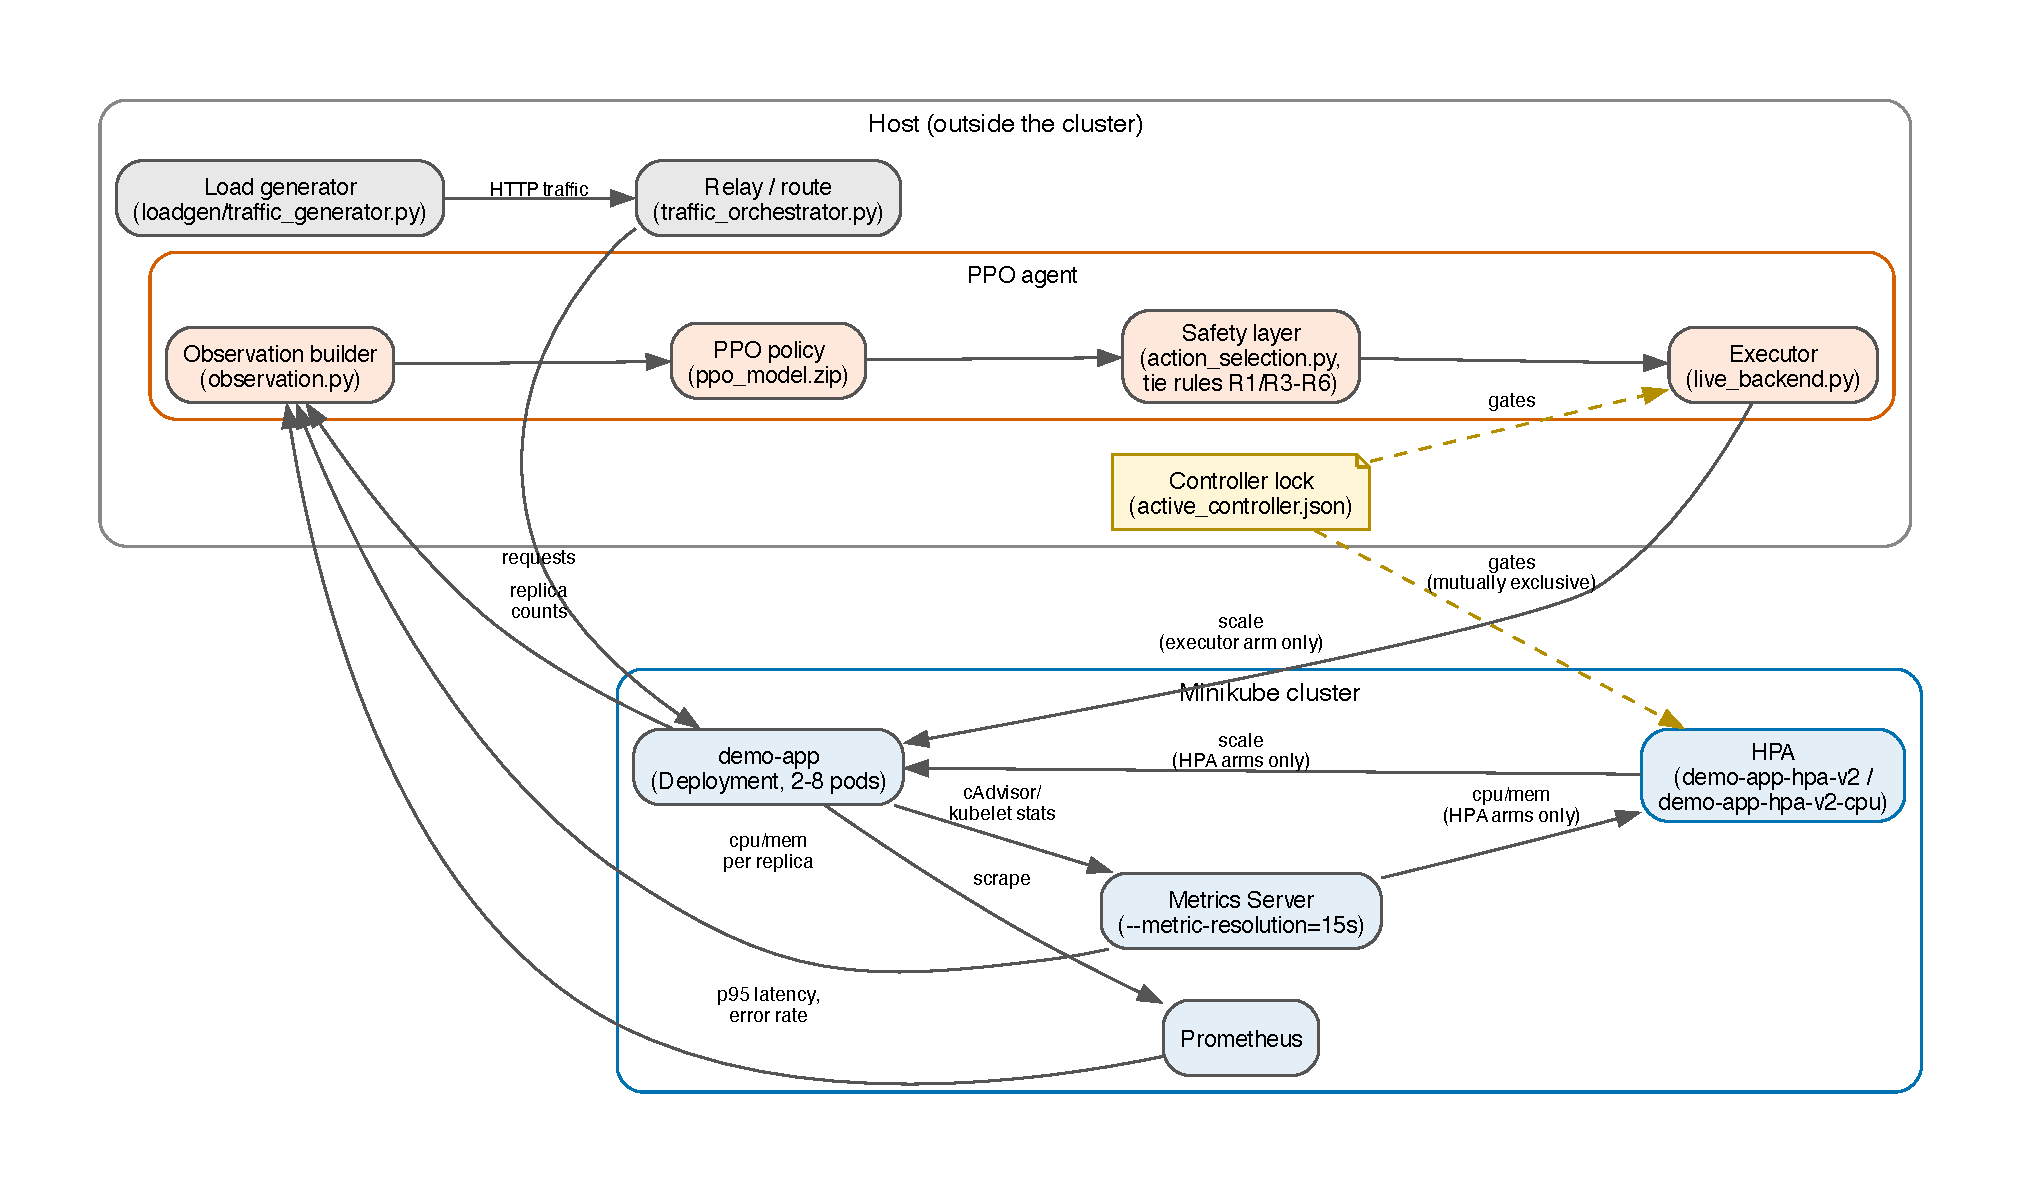
\includegraphics[width=0.95\textwidth]{../figures/diagram_system_architecture.pdf}
\caption{System architecture: the Minikube cluster (demo-app pods, HPA,
Metrics Server at a 15-second resolution, Prometheus) together with the
host-side load generator/relay and the PPO agent's
observation-builder\,$\rightarrow$\,policy\,$\rightarrow$\,safety-layer\,$\rightarrow$\,executor
pipeline, gated by a controller-exclusivity lock so that the PPO agent and
either HPA arm are never both active on the same Deployment at once.}
\label{fig:system-architecture}
\end{figure}

Figure~\ref{fig:rl-control-loop} shows the RL decision loop in isolation:
one 30-second cycle from observation to policy to safety gating to the
Kubernetes API to the resulting metrics to the reward computed from them,
feeding into the next PPO update.

\begin{figure}[htbp]
\centering
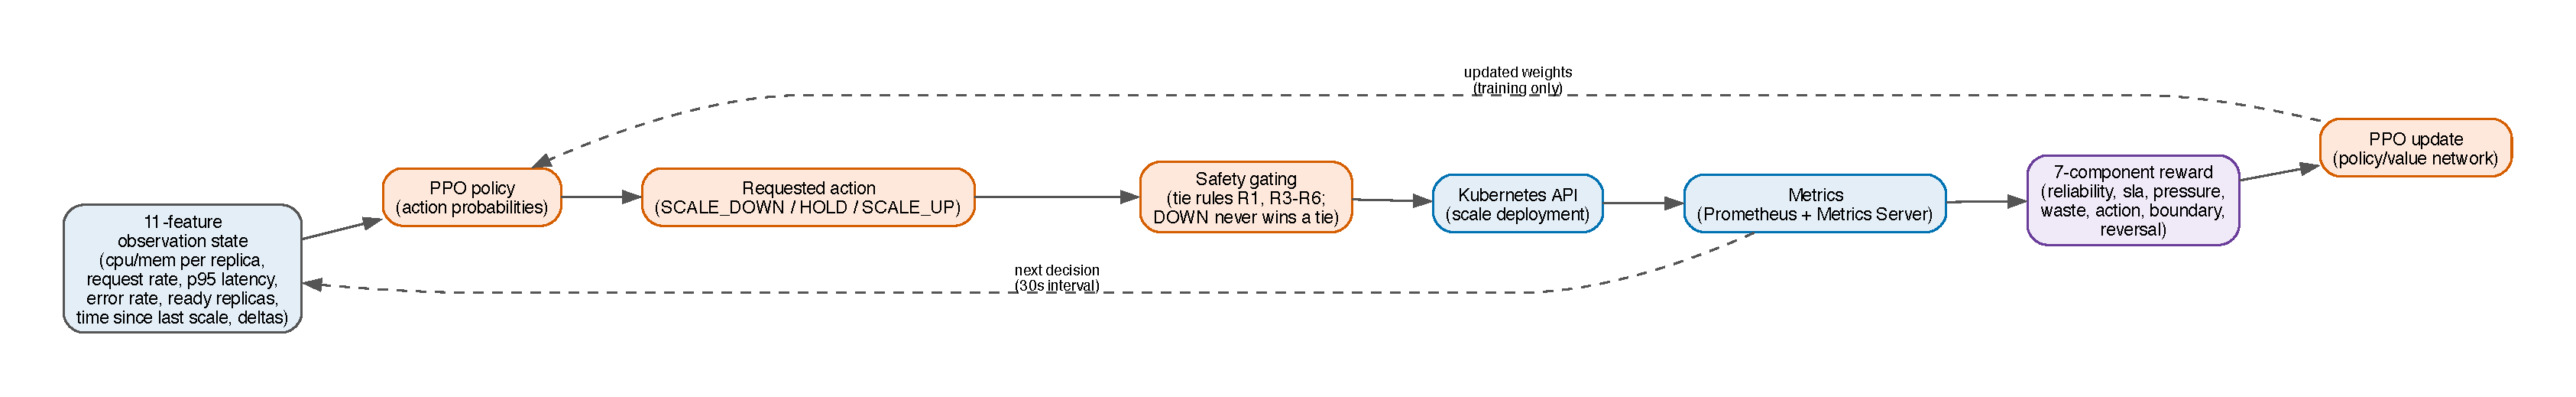
\includegraphics[width=0.85\textwidth]{../figures/diagram_rl_control_loop.pdf}
\caption{The RL control loop: the 11-feature observation feeds the PPO
policy, whose action passes through safety gating before reaching the
Kubernetes API; the resulting metrics feed the 7-component reward, which
feeds the next PPO update. One cycle corresponds to one 30-second decision
interval.}
\label{fig:rl-control-loop}
\end{figure}

Figure~\ref{fig:experiment-pipeline} places the whole project on a single
timeline: the V1 design, its evaluation and failure analysis, the V2
redesign, the 48-session V2 training campaign, the pre-registered V2
evaluation (\texttt{eval\_\allowbreak final}), and the later, separately labelled
exploratory stress test (\texttt{stress\_\allowbreak explore}).

\begin{figure}[htbp]
\centering
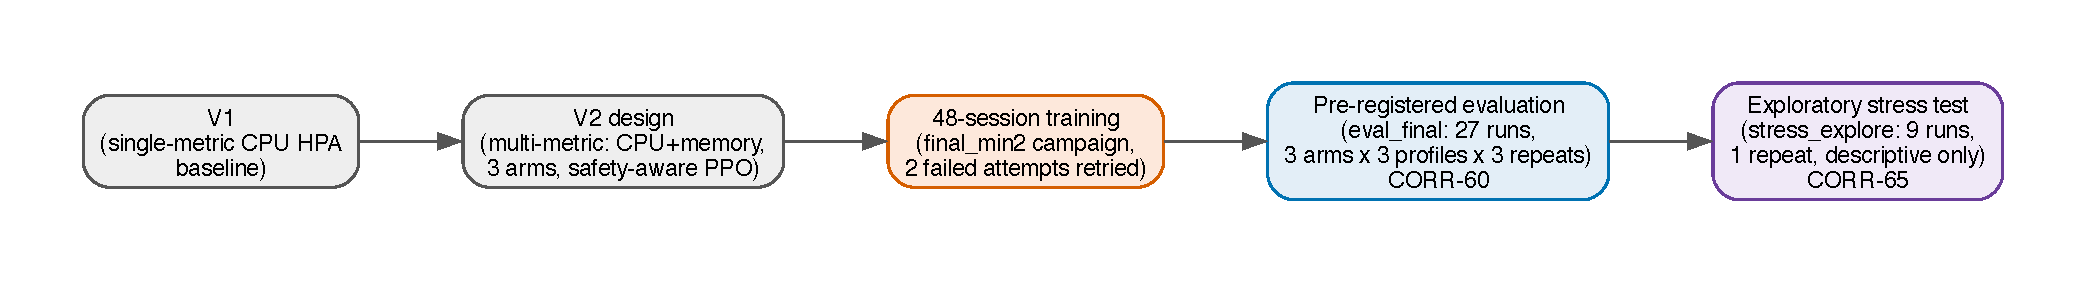
\includegraphics[width=0.9\textwidth]{../figures/diagram_experiment_pipeline.pdf}
\caption{The project's experiment pipeline: V1 design and evaluation,
leading to the V2 redesign, the 48-session V2 training campaign, the
pre-registered evaluation (\texttt{eval\_\allowbreak final}, CORR-60), and the later,
separately labelled exploratory stress test (\texttt{stress\_\allowbreak explore},
CORR-65), which never supersedes the pre-registered evaluation.}
\label{fig:experiment-pipeline}
\end{figure}

\section{Testbed}

We ran every experiment on a single-node Minikube cluster using the Docker
driver, on a MacBook Air with an Apple M1 chip and 8~GB of RAM, with Docker
Desktop providing the container runtime Minikube uses. We allocated 2 CPUs
and 3~GB of RAM to the Minikube virtual node. We chose a local, single-node
cluster over a cloud-hosted or multi-node cluster for a combination of
reasons specific to a capstone project's circumstances rather than any claim
that this is the right choice for production evaluation: it is free, it
gives us full, low-level visibility into node-level CPU and memory pressure
that a managed cluster would partly hide behind another layer of
virtualization, and it let us run both generations' full training and
evaluation campaigns, totalling tens of thousands of real decision steps,
without incurring cloud compute cost or depending on network conditions
outside our control. The obvious limitation of this choice, which we state
plainly in Section~\ref{sec:limitations}, is that a single-node cluster on a
laptop is not a multi-node production cluster, and some findings here (in
particular absolute resource headroom) may not transfer directly.

\section{Benchmark Service}

The benchmark service, in \texttt{app/\allowbreak \allowbreak }, is a small FastAPI application
exposing three endpoints: \texttt{/\allowbreak \allowbreak work}, \texttt{/\allowbreak \allowbreak health}, and
\texttt{/\allowbreak \allowbreak metrics}. The \texttt{/\allowbreak \allowbreak work} endpoint is the one all traffic
profiles target, and it supports two load modes, CPU and memory, selected
per request so that a traffic profile can be built out of a mix of both.
In CPU mode, the handler performs a bounded amount of synchronous
computation sized to hold the request for a target duration, which is what
lets our CPU-oriented traffic profiles push a pod's CPU usage up in a
controlled, repeatable way. In memory mode, the handler allocates and holds
a block of memory for the duration of the request, which is what lets our
memory-oriented profiles (\texttt{eval\_\allowbreak memory\_\allowbreak ramp},
\texttt{stress\_\allowbreak memory\_\allowbreak ramp}) exercise the memory side of the reward and
observation space rather than only CPU. \texttt{/\allowbreak \allowbreak health} is a liveness and
readiness endpoint used by Kubernetes probes; \texttt{/\allowbreak \allowbreak metrics} exposes
Prometheus-format counters and histograms, including request totals by
route, 5xx error totals, request latency, and the number of requests
currently in progress. Each pod is deployed with a CPU request of 100
millicores and a memory request of 64~MiB, with limits of 500 millicores
and 256~MiB; these specific values set the denominators used throughout the
observation space's per-replica ratio features (Section~\ref{sec:mdp}).

\section{Traffic Generator}

The traffic generator, in \texttt{loadgen/\allowbreak \allowbreak }, is open-loop and
deterministic: given a traffic profile and a seed, it produces exactly the
same schedule of requests every time it is replayed, which is what makes a
training session or an evaluation episode reproducible rather than subject
to whatever load the generator happened to produce that run. Being
open-loop means the generator issues requests on its own schedule and does
not slow down or speed up based on how the server is responding, which
mirrors how most real internet traffic behaves and avoids the generator
itself becoming an implicit extra feedback controller that could mask or
distort the autoscaler's own behaviour.

Traffic profiles are organized into four disjoint sets, each firewalled
from the others by an explicit allowlist in the training and evaluation
code so that a profile used for one purpose can never silently leak into
another: a \textbf{training} set used only during the PPO training campaign
(constant CPU, constant memory, constant mixed, mixed ramp, and mixed burst
profiles, cycled through a seeded shuffle); an \textbf{evaluation} set used
only for the pre-registered \texttt{eval\_\allowbreak final} campaign
(\texttt{eval\_\allowbreak cpu\_\allowbreak step}, \texttt{eval\_\allowbreak memory\_\allowbreak ramp},
\texttt{eval\_\allowbreak mixed\_\allowbreak burst}, each peaking at 18-20 requests per second, well
below training-level peaks); a \textbf{stress} set used only for the later,
exploratory \texttt{stress\_\allowbreak explore} campaign (\texttt{stress\_\allowbreak cpu\_\allowbreak burst},
\texttt{stress\_\allowbreak memory\_\allowbreak ramp}, \texttt{stress\_\allowbreak mixed\_\allowbreak burst}, peaking at
45-70 requests per second, at the same peaks already exercised live during
training, never beyond); and a \textbf{demo} set used only by the Streamlit
demonstration console. Table~\ref{tab:eval-profiles} in
Section~\ref{sec:eval-protocol} gives the exact peak rate and resource mode
of each evaluation and stress profile. This firewall exists because the
whole point of an evaluation is to test a controller on traffic it has not
seen; if a profile used in training could also appear in evaluation, even
accidentally, any advantage shown there would be unfalsifiable.

\section{Telemetry and PromQL Signals}

Every signal the RL agent's observation builder uses, and every signal our
evaluation analysis computes, comes from Prometheus, not from the Metrics
Server (the HPA baselines read the Metrics Server for CPU/memory directly,
through the Kubernetes Horizontal Pod Autoscaler controller's own internal
path, which we do not reimplement). The raw metrics read from Prometheus
are: \texttt{demo\_\allowbreak app\_\allowbreak requests\_\allowbreak total} (counter, by route, used via
\texttt{rate()} over a window to get request rate), 5xx error totals (used
the same way to get error rate -- live-observable reliability in this
project is 5xx-only; client-side timeouts and connection errors are not
available to a live policy and are only ever used in offline analysis),
a request latency histogram (used to compute a 95th-percentile, p95,
latency estimate), \texttt{demo\_\allowbreak app\_\allowbreak requests\_\allowbreak in\_\allowbreak progress} (gauge),
container CPU core usage and memory byte usage per pod (from
\texttt{cadvisor}-derived metrics scraped by Prometheus), and the
Deployment's ready and current replica counts, read from the Kubernetes API
rather than Prometheus. We verified the Metrics Server's own resolution at
15 seconds live, immediately before every HPA-arm run, rather than assuming
it; we also verified before every HPA run that Prometheus and the Metrics
Server were both healthy, since both the RL agent and every HPA arm depend
on telemetry being available.

\section{MDP Formulation}
\label{sec:mdp}

We formalize the autoscaling problem as a Markov Decision Process with a
30-second decision interval. At each decision point the agent observes an
eleven-feature vector derived from the raw telemetry above, chooses one of
three actions, and that action -- after passing through the deterministic
safety layer of Section~\ref{sec:safety-layer} -- is applied to the
Deployment's replica count. Thirty seconds later the cycle repeats. One
episode is one full playback of a traffic profile.

\subsection{Observation Features}

Table~\ref{tab:observation-features} gives the eleven observation features
in the exact order the policy network sees them, their raw ranges, how they
are normalized into $[-1,1]$ or $[0,1]$ before being passed to the network,
and whether each is an instantaneous ("current") feature or a trend
feature. Index 0-8 are clipped to their stated raw range and then divided by
that range's width; index 9 (ready replicas) is normalized against the
V2 replica floor and ceiling (2 and 8); index 10 (seconds since the last
effective scaling action) is clipped at a 300-second cap and divided by
that cap. The four trend features (indices 1, 5, 7, and implicitly the
EWMA state behind them) are each the current step's value minus a
90-second exponentially weighted moving average of that same signal, so
that the agent can distinguish "CPU is high and rising" from "CPU is high
and falling" using the same instantaneous value.

\begin{table}[H]
\centering
\caption{The eleven V2 observation features, in network input order.}
\label{tab:observation-features}
\small
\begin{tabular}{p{0.6cm}p{2.6cm}p{6.2cm}p{1.6cm}p{1.7cm}p{1.3cm}}
\hline
index & name & meaning & raw\_range & normalized\_range & temporal \\
\hline
0 & cpu\_per\_replica & (cpu\_cores / ready\_replicas) / 0.100, i.e. fraction of the 100m CPU request per Ready replica -- a NOMINALLY COMPARABLE proxy to HPA's averageUtilization/100, not literally identical to it (docs/rl\_mdp\_spec.md sec.4, CORR-27). & [0.0, 5.0] & [0.0, 1.0] & current \\
1 & cpu\_per\_replica\_delta & current step's cpu\_per\_replica minus its 90s EWMA (momentum/trend, not a raw one-step difference). & [-5.0, 5.0] & [-1.0, 1.0] & trend \\
2 & memory\_per\_replica & (memory\_bytes / ready\_replicas) / 67108864, i.e. fraction of the 64MiB memory request per Ready replica. & [0.0, 4.0] & [0.0, 1.0] & current \\
3 & in\_progress\_per\_replica & requests\_in\_progress / ready\_replicas -- secondary queueing-pressure signal, redundant with CPU on this CPU-bound app but retained per Phase 15A evaluation for robustness. & [0.0, 20.0] & [0.0, 1.0] & current \\
4 & request\_rate\_norm & sum(\allowbreak rate(\allowbreak demo\_app\_requests\_total\allowbreak \{route="/work"\}[1m])), normalized against a 100 RPS design ceiling, justified ONLY from non-held-out development profile peaks (burst=70, ramp=60, step=50 RPS). Never justified from any held-out evaluation workload's parameters (CORR-27; see docs/rl\_mdp\_spec.md sec.22). & [0.0, 100.0] & [0.0, 1.0] & current \\
5 & request\_rate\_delta & current step's request\_rate\_rps minus its 90s EWMA. & [-100.0, 100.0] & [-1.0, 1.0] & trend \\
6 & p95\_latency\_norm & latency\_p95\_seconds (ms), normalized against a 2000ms ceiling (~6.67x the 300ms SLA target). If request\_rate\_rps==0 with no histogram observations, this is semantically 0ms ("no\_traffic", CORR-27) -- not a telemetry failure; see docs/rl\_mdp\_spec.md sec.6. & [0.0, 2000.0] & [0.0, 1.0] & current \\
7 & p95\_latency\_delta & current step's p95 latency (ms) minus its 90s EWMA. & [-2000.0, 2000.0] & [-1.0, 1.0] & trend \\
8 & error\_rate & error\_rate\_rps (5xx only, live-observable) / request\_rate\_rps; 0.0 if request\_rate\_rps==0; null (missing) if request\_rate\_rps is null. & [0.0, 1.0] & [0.0, 1.0] & current \\
9 & ready\_replica\_norm & (replicas\_ready - 2) / (8 - 2) -- authoritative physical capacity, never hpa\_status\_current\_replicas (CORR-25). Normalized against a replica floor of 2 and ceiling of 8 (CORR-55); the floor is 2, never 1. & [2.0, 8.0] & [0.0, 1.0] & current \\
10 & seconds\_since\_last\_scale\_norm & controller-tracked seconds since the last EFFECTIVE (non-HOLD) action, capped per experiment.yaml rl.time\_since\_scale\_cap\_seconds. & [0.0, 300.0] & [0.0, 1.0] & current \\
\hline
\end{tabular}

\end{table}

\subsection{Normalization and Missing-Data Rules}
\label{sec:invalid-telemetry}

Two distinct situations have to be told apart carefully, and conflating
them was a source of an early V1-era bug (CORR-56) that we describe in
Section~\ref{sec:v1-to-v2}: genuine zero traffic, and missing or unreliable
telemetry. When the request rate is genuinely zero and no latency
histogram observations exist for the window, the p95 latency feature is
defined as exactly 0~ms -- this is a valid, meaningful state ("no traffic
right now"), not a sign that something is wrong, and it participates
normally in the EWMA trend calculation. When the request rate is nonzero
but a usable latency estimate cannot be computed, or any other required raw
signal cannot be read for the window, the sample is marked invalid; on an
invalid sample, every level and trend feature except the two
controller-tracked ones (ready-replica count and seconds-since-last-scale,
both of which come from state the controller itself always knows,
independent of Prometheus) holds its previous normalized value rather than
being set to zero, the clip maximum, or any other fabricated number. The
very first decision of an episode, before any previous value exists, uses
the raw-range midpoint for every held feature and is flagged as such. Four
consecutive invalid decisions (two minutes of persistently unusable
telemetry at the 30-second interval) terminate the episode; one to three
consecutive invalid decisions instead force a deterministic HOLD action for
that step, through the same safety layer that governs every other case
requiring a fallback.

\section{Action Space and Safety Layer}
\label{sec:safety-layer}

The action space is \texttt{Discrete(3)}: remove one replica
(\textsc{scale\_down\_one}), hold the current replica count
(\textsc{hold}), or add one replica (\textsc{scale\_up\_one}). The policy
network never outputs a replica count directly and never outputs a
multi-replica jump; every decision changes the Deployment by at most one
replica, which keeps the action space small and keeps every single action's
effect easy to reason about and to log.

Between the policy's raw action and the Kubernetes API sits a deterministic
safety layer that the learned policy cannot see into or override. Its rules
are, in the order they are checked: a replica-bound clamp, so that a
requested delta that would take the Deployment below the configured floor
or above the configured ceiling is converted to a no-op with that clamp
recorded as the override reason; a pending-scale gate, so that if the
Deployment's desired and ready replica counts currently disagree (a scaling
action is already in flight), any further non-hold action is overridden to
hold until the pending change settles; and an asymmetric cooldown, so that
a scale-up action is never delayed by this gate beyond ordinary pending-scale
settling, while a scale-down action additionally requires at least 60
seconds to have passed since the last effective scaling action of any
direction. This asymmetry is deliberate: it lets the controller react to a
sudden spike immediately, in either generation's design, while making
scaling down a more deliberate, slower action that cannot immediately
reverse an upward move -- the asymmetric cooldown further explicitly allows
an "emergency reversal" (an immediate scale-up right after a scale-down) to
pass through ungated, since erring toward more capacity is never penalized
by this gate. Listing~\ref{lst:gating} in Appendix~\ref{ch:appendix} gives
the gating function in full.

\subsection{Safety-Aware Tie-Breaking}
\label{sec:tie-break}

A separate concern from gating is what the controller should do when the
policy's own output does not clearly favour one action. For deterministic
evaluation, Stable-Baselines3's default behaviour is to take the
arg-max of the policy's action probabilities; when two or more actions are
within a small margin of each other, an arg-max breaks the tie toward the
lowest action index, which in our action encoding is
\textsc{scale\_down\_one} -- meaning an uncertain policy would be silently
biased toward removing capacity purely as an artefact of how ties are
broken, never because removing capacity was actually the better action
on the merits. We replaced this default with a safety-aware tie-break rule
(CORR-58), used only for deterministic inference during evaluation, never
during training (Stable-Baselines3's own stochastic sampling during
\texttt{model.learn()} never passes through this code path). The rule
first computes the tie set: every action whose probability is within
$\varepsilon$ of the maximum probability. If the tie set has exactly one
member, that action is chosen (rule R1) and the controller's own inference
log records this as "no tie," which is what happens on the overwhelming
majority of decisions. If the tie set is larger than one, the following
rules apply, in order, and are illustrated in
Figure~\ref{fig:tie-break-flow}:

\begin{itemize}[nosep]
  \item \textbf{R2}: \textsc{scale\_down\_one} can never, by construction,
    be the output of a tie -- it structurally never wins when tied with
    anything else.
  \item \textbf{R3}: a tie between \textsc{hold} and
    \textsc{scale\_up\_one} resolves to \textsc{scale\_up\_one} if the
    system is currently judged \emph{stressed}, and to \textsc{hold}
    otherwise.
  \item \textbf{R4}: a tie between \textsc{scale\_down\_one} and
    \textsc{scale\_up\_one}, or a three-way tie among all actions, resolves
    to \textsc{hold}.
  \item \textbf{R5}: a tie between \textsc{scale\_down\_one} and
    \textsc{hold} resolves to \textsc{hold}.
  \item \textbf{R6}: if whether the system is stressed cannot be determined
    (for example, because the raw observation needed to judge it is itself
    missing), the rule fails safe to \textsc{hold}.
\end{itemize}

\begin{figure}[htbp]
\centering
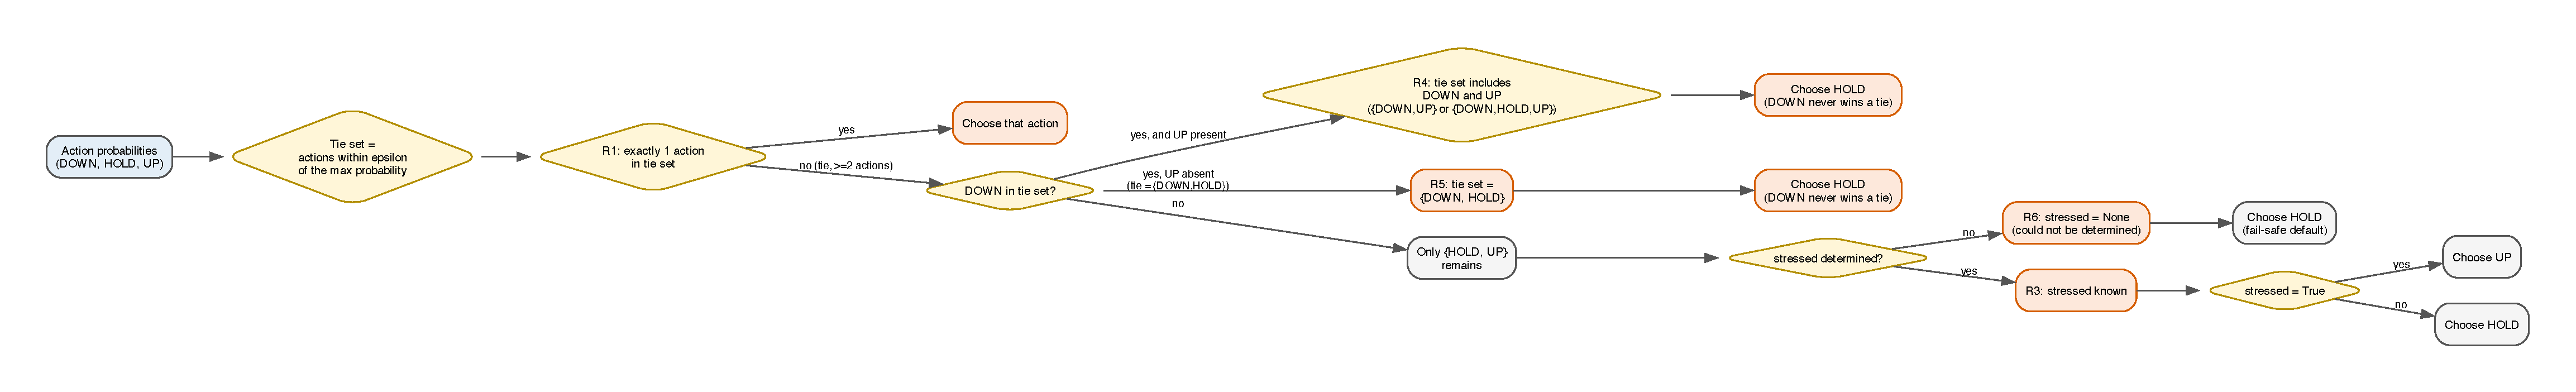
\includegraphics[width=0.78\textwidth]{../figures/diagram_tie_break_flow.pdf}
\caption{Decision flow for the safety-aware tie-break rule (R1-R6,
CORR-58): from the PPO action-probability tie set to the final selected
action. \textsc{scale\_down\_one} can never win a tie by construction; an
unknown-stress tie fails safe to \textsc{hold}.}
\label{fig:tie-break-flow}
\end{figure}

"Stressed" is defined from the same decision-time raw observation the
policy itself sees: the system is stressed if p95 latency is at or above
the SLA target, or the error rate is above zero, or CPU or memory per ready
replica is above its configured "safe-high" threshold (the same thresholds
used in the V2 pressure reward term, Section~\ref{sec:v2-reward}). The
intent, stated in our own design-correction log, is availability-first
behaviour under genuine stress -- scale up quickly when the signals say the
system is actually under load, roughly mirroring how a conventional HPA
would react -- while never letting scale-down be the accidental outcome of
an uncertain policy rather than a deliberate one.

\subsection{Epsilon Calibration}

The tie-break margin $\varepsilon$ was calibrated, not guessed, and
calibrated before the pre-registered evaluation it would be used in, not
after. We computed the margin between each decision's top and second
probability over the final training checkpoint's behaviour on the last
five training sessions (sessions 43-47), took the 10th percentile of that
margin distribution, and capped the result at 0.05 (floored at 0.0). The
raw 10th-percentile value came out above the cap, so the calibrated
$\varepsilon$ used throughout evaluation is 0.05. Only 0.55\% of decisions
in that calibration window fell inside a tie at this value, and in the
actual pre-registered evaluation, the tie-break rule changed the outcome of
only 4 of 360 PPO decisions (1.11\%; Figure~\ref{fig:tie-rule-frequency} in
Chapter~\ref{ch:results}) -- the safety-aware rule is a rare, deliberately
narrow intervention, not a mechanism that drives most decisions.

\section{V1 Reward Function}
\label{sec:v1-reward}

V1's reward combined a latency penalty, an error penalty, an unconditional
per-replica resource cost, small action/reversal/boundary penalties, and a
positive "efficiency" bonus. In the exact form frozen for V1
(\texttt{docs/\allowbreak \allowbreak rl\_\allowbreak mdp\_\allowbreak spec.md}, \texttt{rl\_\allowbreak contract\_\allowbreak version 2},
CORR-27):
\begin{equation}
r_t = -\min(e_t^2, 4) - 5\rho_t - \frac{n_t-1}{7} - 0.1\,\mathbb{1}_{\text{act}} - 0.5\,\mathbb{1}_{\text{rev}} - 0.2\,\mathbb{1}_{\text{bnd}} + 0.3\,\mathbb{1}_{\text{eff}}
\label{eq:v1-reward}
\end{equation}
where $e_t = \max(0, p_t - 300)/300$ is the fractional excess of p95 latency
$p_t$ (in milliseconds) above a 300~ms target, $\rho_t$ is the 5xx error
fraction, $n_t$ is the current replica count (so the resource term grows
toward 1 as replicas approach the 8-replica ceiling and is paid on
\emph{every} step regardless of whether the extra replicas are doing any
good), and the indicator terms penalize taking any non-hold action, any
direction reversal within a window, and any action clamped at a replica
bound; the efficiency bonus rewards a step where CPU per replica sits
between $1.0\times$ and $3.0\times$ the CPU request, latency is below
target, and there are no errors. The critical property of
Equation~\ref{eq:v1-reward} for what follows is the unconditional resource
term $-(n_t-1)/7$: it charges a cost for every replica above one,
\emph{every single step}, whether or not the system actually needed those
replicas, and it does so regardless of the pod health that produced that
replica count.

\section{PPO Algorithm and Hyperparameters}

Both generations used the same PPO implementation (Stable-Baselines3
\cite{raffin2021sb3}) and the same core hyperparameters, summarized in
Table~\ref{tab:ppo-hyperparams}, with a two-layer, 128-unit multilayer
perceptron for both the policy and value networks, no hyperparameter
search performed, and a fixed training seed (42) throughout. One detail
specific to this project's live-cluster setting is the rollout length: PPO
defaults in Stable-Baselines3 to collecting 2048 steps between updates,
which at a 30-second decision interval would mean roughly 17 hours between
updates; we instead collect 256 steps (one "session") between updates, so
that each training session completes in a practical wall-clock time and
checkpoints at a useful cadence, at the cost of each PPO update seeing a
smaller batch of fresh experience than the library's own default assumes.

\begin{table}[H]
\centering
\caption{PPO hyperparameters used for both V1 and V2 training.}
\label{tab:ppo-hyperparams}
\begin{tabular}{ll}
\hline
parameter & value \\
\hline
learning\_rate & 0.0003 \\
n\_steps & 2048 \\
batch\_size & 64 \\
n\_epochs & 10 \\
gamma & 0.99 \\
gae\_lambda & 0.95 \\
clip\_range & 0.2 \\
ent\_coef & 0.01 \\
vf\_coef & 0.5 \\
max\_grad\_norm & 0.5 \\
policy & MlpPolicy \\
net\_arch & [128, 128] \\
training\_budget & 48 sessions x 256 steps/session = 12288 total timesteps (final\_min2 campaign) \\
\hline
\end{tabular}

\end{table}

\section{Session, Checkpoint, and Resume Design}

Training proceeds in sessions of 256 decision steps each; every session
ends with a Stable-Baselines3 checkpoint (\texttt{ppo\_\allowbreak model.zip}), the
environment's own random-number-generator state (so a resumed session
reproduces the same stochastic choices it would have made had it not
stopped), and session metadata recording cumulative timesteps, cumulative
PPO updates, and which sessions have completed. A campaign can be resumed
from its last completed session rather than restarted from scratch, which
matters in practice: of the V2 campaign's 48 planned sessions, two
(sessions 4 and 38) failed partway through and had to be resumed from the
last good checkpoint rather than from session zero, a design choice that
turned a potential multi-day restart into a same-day recovery. We discuss
both failures, and what caused them, in Chapter~\ref{ch:results}.

\section{Freeze Manifest, Correction Log, and Pre-Registration}

Three documents together are this project's reproducibility methodology,
and we treat them as load-bearing rather than as paperwork. The
\textbf{freeze manifest} (\texttt{FREEZE\_\allowbreak MANIFEST.json}, with two later
amendments) records SHA-256 hashes of every file governing a training
campaign -- the environment code, the reward implementation, the
configuration files, the PPO hyperparameters, the live cluster's resource
limits at freeze time -- at the moment the final V2 campaign began; any
post-freeze change to a hashed file invalidates that campaign's checkpoints
for resumption, verified automatically rather than trusted to memory. The
\textbf{correction log} (\texttt{docs/\allowbreak \allowbreak experimental\_\allowbreak design\_\allowbreak corrections.md})
is an append-only record of every design decision and mid-course
correction made across the whole project, numbered CORR-1 through CORR-65,
each with its problem, decision, scope, scientific impact, and
non-retroactivity explicitly stated; nothing in this project is corrected
silently, and a reader can always find out exactly when and why a given
rule changed. The \textbf{pre-registration}
(\texttt{docs/\allowbreak \allowbreak evaluation\_\allowbreak v2\_\allowbreak preregistration.md}, CORR-60) fixes the
evaluation's arms, traffic profiles, metrics, retry rules, and decision
rule in writing before any V2 evaluation episode ran -- before the final
training checkpoint (session 47) even existed. We refer back to specific
CORR entries throughout this chapter and the next, both because they are
the authoritative source for each design decision and because a reader
who wants the full detail behind a short summary here can look it up by
number; Appendix~\ref{ch:appendix} gives a complete table of every CORR
entry.

\section{V1 to V2 Redesign}
\label{sec:v1-to-v2}

V1's evaluation (Chapter~\ref{ch:results}) did not produce a usable
PPO-versus-HPA verdict: of three required valid PPO repeats, only one
completed without a safety termination. Diagnosing why led to the V2
redesign summarized in Table~\ref{tab:v1-v2-comparison}; none of these
changes were made casually, and each is backed by a numbered correction in
the log.

\begin{table}[H]
\centering
\caption{Design differences between V1 and V2, and the reason for each.}
\label{tab:v1-v2-comparison}
\small
\begin{tabular}{p{2.6cm}p{2.9cm}p{2.9cm}p{4.3cm}}
\toprule
Aspect & V1 & V2 & Reason for the change \\
\midrule
Observation signals & CPU-derived only (1 primary dimension) & 11 features: CPU, memory, request rate, latency, replica state, all 4 with short-horizon trends & A CPU-only view cannot represent memory-bound load or anticipate a trend; V2's benchmark service and traffic profiles deliberately exercise memory as well as CPU. \\
Replica floor & 1 & 2 (CORR-55) & Both live V1-era attempts at scientific session index 3 of V2 final training failed with the Deployment's entire ready-replica count driven to zero by a single pod's own saturation or restart -- a floor of 1 gives the whole system no redundancy against one pod's transient unhealthiness. \\
Resource/waste cost & Unconditional, every step, proportional to replica count & Conditional "waste" penalty, fires only when replicas exceed the floor \emph{and} CPU/memory are both low \emph{and} latency/error are already healthy & V1's unconditional cost made adding a replica look bad even when the system genuinely needed it, biasing the policy toward staying small regardless of actual load. \\
SLA target (p95) & 300\,ms & 1000\,ms (CORR-57) & Memory-mode requests legitimately hold for close to 500\,ms; combined with Prometheus histogram-bucket interpolation, this was being reported near 975\,ms and permanently penalized against a 300\,ms target that the workload could not realistically meet. \\
Deterministic tie-break & SB3 default arg-max (ties toward lowest action index, i.e.\ scale-down) & Safety-aware rule, scale-down can never win a tie (CORR-58) & An uncertain policy should never have its uncertainty silently resolved toward removing capacity. \\
Comparison baseline(s) & One tuned HPA (CPU only) & Two HPA arms: CPU+memory (resource baseline) and CPU-only (CPU baseline), both at the V2 floor of 2 (CORR-62) & Isolates whether the memory metric matters and whether the higher replica floor alone explains any difference, rather than conflating both changes in a single baseline. \\
Training budget & 5,120 timesteps (20 sessions), cut short by live-cluster wall-clock constraints & 12,288 timesteps (48 sessions), amended and recorded before any post-amendment session result existed (CORR-59) & V1's budget was not a deliberate scientific choice; V2's budget change was decided and logged while only session 0 had been reviewed, avoiding an outcome-aware budget increase. \\
\bottomrule
\end{tabular}
\end{table}

\section{V2 Reward Function}
\label{sec:v2-reward}

The V2 reward replaces V1's unconditional resource cost and latency-only
penalty with seven components, each independently weighted, summarized in
Table~\ref{tab:reward-components} and defined in full in
\texttt{configs/\allowbreak \allowbreak reward\_\allowbreak v2.yaml} (Listing~\ref{lst:reward-config} in
Appendix~\ref{ch:appendix}):
\begin{equation}
r_t = -\big(w_{\text{rel}}\rho_t + w_{\text{sla}}\,\mathrm{sla}_t + w_{\text{prs}}\,\mathrm{prs}_t + w_{\text{wst}}\,\mathbb{1}_{\text{waste}} + w_{\text{act}}\,\mathbb{1}_{\text{act}} + w_{\text{rev}}\,\mathbb{1}_{\text{rev}} + w_{\text{bnd}}\,\mathbb{1}_{\text{bnd}}\big)
\label{eq:v2-reward}
\end{equation}
with $\rho_t$ the clipped 5xx error fraction; $\mathrm{sla}_t =
\mathrm{clip}(e_t^2, 0, 1)$ the clipped squared excess of p95 latency above
the 1000~ms target, $e_t = \max(0, p_t-1000)/1000$; and
$\mathrm{prs}_t = \max(\mathrm{prs}_{\text{cpu}}, \mathrm{prs}_{\text{mem}})$
the worse of a CPU and a memory "pressure" term, each defined as the
clipped, squared fraction of the way a per-replica utilization has moved
from a "safe-high" threshold toward a hard resource limit:
$\mathrm{prs}_{\text{cpu}} = \mathrm{clip}\!\left(\frac{u_{\text{cpu}} -
3.0}{5.0-3.0}, 0, 1\right)^2$ and similarly for memory with thresholds
1.2 and 4.0. The waste indicator fires only when the current replica count
is above the floor \emph{and} CPU and memory per replica are both below
their waste thresholds \emph{and} latency and error are already healthy --
by construction, a policy cannot lower its waste cost by staying small
while the system is in genuine distress, because the waste term simply does
not apply in that state. Action, reversal, and boundary penalties are
unchanged in shape from V1.

\begin{table}[H]
\centering
\caption{V2 reward components, weights, and threshold parameters.}
\label{tab:reward-components}
\small
\begin{tabular}{p{2cm}p{1cm}p{7.2cm}p{4.3cm}}
\hline
component & weight & meaning & threshold\_params \\
\hline
w\_reliability & 6.0 & Penalizes the live 5xx error rate (clipped to [0,1]). & n/a \\
w\_sla & 4.0 & Penalizes squared excess p95 latency above the SLA target (clipped to [0,1]). & p95\_target\_ms=1000 \\
w\_pressure & 2.0 & Penalizes the worse of CPU/memory 'unsafe pressure' (distance toward the pod's hard resource limit). & cpu\_safe\_high=3.0, cpu\_hard\_limit=5.0, memory\_safe\_high=1.2, memory\_hard\_limit=4.0 \\
w\_waste & 0.3 & Penalizes over-provisioning (replicas > floor, low CPU+memory, SLA/error already healthy). & cpu\_waste\_threshold=1.0, memory\_waste\_threshold=1.0 \\
w\_action & 0.1 & Penalizes taking any non-HOLD action (discourages unnecessary churn). & per\_action\_cost=1.0 \\
w\_reversal & 0.5 & Penalizes reversing a scaling direction within the reversal window (discourages oscillation). & reversal\_window\_seconds=120, per\_reversal\_cost=1.0 \\
w\_boundary & 0.2 & Penalizes an action clamped at the replica floor/ceiling (discourages pushing against the bound). & per\_boundary\_violation\_cost=1.0 \\
\hline
\end{tabular}

\end{table}

\section{Evaluation Protocol}
\label{sec:eval-protocol}

\subsection{Arms and Profiles}

Table~\ref{tab:eval-arms} lists the three arms compared in both the
pre-registered evaluation and the exploratory stress test; all three use
identical replica bounds (2-8) and the identical benchmark application
image, so that the only thing that differs between arms is the controller
itself. Table~\ref{tab:eval-profiles} lists the traffic profiles each
campaign uses.

\begin{table}[H]
\centering
\caption{Evaluation arms.}
\label{tab:eval-arms}
\resizebox{\linewidth}{!}{\begin{tabular}{lll}
\hline
arm & profiles\_run\_on & role \\
\hline
PPO (multi-metric, 11 signals) & all 3 held-out + all 3 stress & RL policy under test \\
HPA CPU+Memory & all 3 held-out + all 3 stress & resource-metric baseline (CPU and memory, 260\%/120\% targets) \\
HPA CPU-only (CPU baseline) & all 3 held-out + all 3 stress & single-metric baseline (CPU only, same 260\% target and 2-8 bounds as the others) \\
\hline
\end{tabular}
}
\end{table}

\begin{table}[H]
\centering
\caption{Traffic profiles used by the pre-registered evaluation
(\texttt{eval\_\allowbreak final}) and the exploratory stress test
(\texttt{stress\_\allowbreak explore}).}
\label{tab:eval-profiles}
\resizebox{\linewidth}{!}{\begin{tabular}{lllll}
\hline
campaign & profile & resource\_mode & peak\_rps & repeats \\
\hline
eval\_final (pre-registered, CORR-60) & eval\_cpu\_step & cpu & 18.0 & 3 \\
eval\_final (pre-registered, CORR-60) & eval\_memory\_ramp & memory & 18.0 & 3 \\
eval\_final (pre-registered, CORR-60) & eval\_mixed\_burst & mixed & 20.0 & 3 \\
stress\_explore (exploratory, CORR-65) & stress\_cpu\_burst & cpu & 70.0 & 1 \\
stress\_explore (exploratory, CORR-65) & stress\_memory\_ramp & memory & 45.0 & 1 \\
stress\_explore (exploratory, CORR-65) & stress\_mixed\_burst & mixed & 70.0 & 1 \\
\hline
\end{tabular}
}
\end{table}

\subsection{Design and Order}

The pre-registered \texttt{eval\_\allowbreak final} campaign ran 3 repeats of every
(profile, arm) cell: 3 profiles $\times$ 3 arms $\times$ 3 repeats = 27
planned runs. The order of the three arms within each repeat was rotated
using a Latin square, so that no arm was systematically run first or last
within a repeat -- a precaution against any systematic drift in cluster
state (for example, residual caching or thermal effects) that could
otherwise confound arm identity with run order. Before every HPA-arm run we
verified Metrics Server resolution and cluster health live rather than
assuming them, and Grafana was scaled to zero replicas for the whole V2
evaluation campaign so that it could not compete with the benchmark
application for the Minikube node's limited CPU and memory, and so that it
could not itself add any confounding load to the cluster during a
measured run.

\subsection{Metrics and Decision Rule}

The primary metrics, fixed in the pre-registration before any evaluation
run, are SLA-violation rate at the 1000~ms target and replica-minutes (the
time-integral of replica count, our cost proxy). Secondary metrics include
mean and median p95 latency, error rate, maximum per-pod memory, scaling
action count, reversal count, pod restart count, invalid-sample count, and
an SLA-violation rate at a 300~ms reference threshold kept only for
historical comparability with V1. Table~\ref{tab:decision-rule} states the
decision rule exactly as pre-registered: an arm is only reported as
"better" than another on a given metric for a given profile if it is
better in all three of the three repeats, and no single aggregate winner is
declared when different metrics disagree -- such cases are reported
explicitly as a trade-off rather than resolved into one ranking.

\begin{table}[H]
\centering
\caption{Pre-registered decision rule (CORR-60).}
\label{tab:decision-rule}
\small
\begin{tabular}{p{3cm}p{12cm}}
\hline
rule & statement \\
\hline
reporting & Per profile, per arm: report mean +/- standard deviation over the 3 repeats for every metric. \\
claiming\_better & An arm may be claimed 'better' than another on a given metric for a given profile ONLY if it is better in ALL 3 of the 3 repeats (not merely on average) -- a single repeat going the other way blocks the claim for that metric/profile pair. \\
no\_aggregate\_winner & No single aggregate 'winner' is declared across metrics that disagree (e.g. one arm has a lower SLA-violation rate but higher replica-minutes) -- such cases are reported explicitly as a trade-off, not resolved into a single ranking. \\
applies\_to & eval\_final only (3 repeats/cell). Does NOT apply to stress\_explore (1 repeat/cell, descriptive only, CORR-65). \\
\hline
\end{tabular}

\end{table}

\subsection{Retry Rules}

A tooling failure -- an unreachable route, a down Prometheus instance, a
cluster or network fault, none of which reflects anything about either
controller's scaling behaviour -- results in no scientific outcome being
recorded for that attempt and exactly one retry; the failed attempt's
evidence is preserved, never deleted. A safety termination (a sustained
loss of ready replicas, or a memory threshold breach) is, by contrast,
counted as a real scientific outcome of that run and is never retried,
because a safety termination is itself a fact about how the controller
behaved under that traffic, not a tooling artefact to be papered over.

\section{The Demo UI}

\texttt{demo\_\allowbreak ui/\allowbreak \allowbreak } is a Streamlit console used to inspect training curves,
replay evaluation episodes, and view live cluster state during
development and demonstration. It runs in a demo/fixture mode by default
and does not require a live cluster to start, falling back to cached or
fixture data when a live connection is unavailable, so that it can be used
for a demonstration without first standing up the full testbed. It reads
the same \texttt{persistent-data/\allowbreak \allowbreak } artifacts (training session metadata,
evaluation run ledgers) that the analysis scripts in
Section~\ref{sec:software-stack} read, rather than maintaining its own
separate copy of this data, so that what the UI shows and what the
published figures and tables show cannot drift apart.

\section{Software Stack and Hardware}
\label{sec:software-stack}

Table~\ref{tab:software-stack} lists the key software dependencies and the
exact versions pinned in the project's requirements files.
Table~\ref{tab:hardware} lists the hardware used for every training and
evaluation run reported in this document.

\begin{table}[H]
\centering
\caption{Key software dependencies and pinned versions.}
\label{tab:software-stack}
\begin{tabular}{ll}
\toprule
Component & Version \\
\midrule
Python & 3.10.14 \\
Kubernetes Python client & 31.0.0 \\
FastAPI & 0.115.6 \\
Uvicorn & 0.32.1 \\
Prometheus client (Python) & 0.21.1 \\
prometheus-api-client & 0.5.5 \\
NumPy & 1.26.4 \\
Pandas & 2.2.3 \\
Stable-Baselines3 & 2.6.0 \\
Gymnasium & 1.1.1 \\
PyTorch & 2.5.1 \\
Matplotlib & 3.10.9 \\
scikit-learn & 1.6.1 \\
Streamlit (demo UI) & 1.65.0 \\
Plotly (demo UI) & 7.1.0 \\
\bottomrule
\end{tabular}
\end{table}

\begin{table}[H]
\centering
\caption{Hardware used for all training and evaluation runs.}
\label{tab:hardware}
\begin{tabular}{ll}
\toprule
Item & Specification \\
\midrule
Host laptop & MacBook Air, Apple M1, 8\,GB RAM \\
Container runtime & Docker Desktop \\
Kubernetes cluster & Minikube, single node, Docker driver \\
Cluster CPU allocation & 2 vCPU \\
Cluster memory allocation & 3\,GB \\
\bottomrule
\end{tabular}
\end{table}

\section{Integration and Workflow}

Putting the pieces together, a single evaluation attempt proceeds as
follows: the harness runs a preflight check (cluster, Prometheus, Metrics
Server health); it acquires the arm's controller identity under the
exclusivity lock, deleting any HPA object left behind by a previous arm so
that a stale controller cannot interfere; it starts the traffic generator
against the configured profile; the active controller (PPO or one of the
two HPA configurations) scales the Deployment for the length of the
episode; telemetry is recorded throughout; the generator is stopped and
drained; the cluster is cleaned up and settled back to canonical idle
state; and the attempt's full result, success or failure, is written to the
run's own directory and to the campaign's ledger. The same orchestration
code path, \texttt{scripts/\allowbreak \allowbreak evaluate\_\allowbreak v2\_\allowbreak campaign.py}, runs both the
pre-registered evaluation and the later exploratory stress test, differing
only in which traffic profiles and repeat counts are configured, which is
part of why we can state confidently that the two campaigns are run under
identical operational discipline even though their scientific status (a
decision-rule-bearing evaluation versus a descriptive, single-repeat
exploration) is very different.

\chapter{Cost Analysis}
\label{ch:cost}

\section{Hardware Requirements}
\label{sec:cost-hardware}

Table~\ref{tab:cost-hardware} lists the hardware used to build and run this
project. No hardware was purchased specifically for this project; the
laptop was already owned before the project began.

\begin{table}[H]
\centering
\caption{Hardware requirements.}
\label{tab:cost-hardware}
\begin{tabular}{lll}
\toprule
Item & Specification & Status \\
\midrule
Laptop & MacBook Air, Apple M1, 8\,GB RAM, 256\,GB SSD & Already owned \\
Internet connection & Broadband, for package/image downloads & Already available \\
\bottomrule
\end{tabular}
\end{table}

\section{Software Requirements}
\label{sec:cost-software}

Table~\ref{tab:cost-software} lists the software this project depends on.
Every item is open-source and free to use; none required a paid licence
or subscription.

\begin{table}[H]
\centering
\caption{Software requirements.}
\label{tab:cost-software}
\begin{tabular}{lll}
\toprule
Item & Role & Licence cost \\
\midrule
Docker Desktop & Container runtime for Minikube & Free (personal use) \\
Minikube & Single-node Kubernetes cluster & Free, open source \\
kubectl, Helm & Cluster administration & Free, open source \\
kube-prometheus-stack & Prometheus and Grafana & Free, open source \\
Python 3.10 & Runtime for all project code & Free, open source \\
Stable-Baselines3, Gymnasium, PyTorch & RL training/inference & Free, open source \\
FastAPI, Uvicorn & Benchmark service & Free, open source \\
Streamlit, Plotly & Demo UI & Free, open source \\
Matplotlib, Graphviz & Figures and diagrams & Free, open source \\
\bottomrule
\end{tabular}
\end{table}

\section{List of Components and Their Cost}
\label{sec:cost-components}

Table~\ref{tab:cost-total} itemizes cost by component. Because the laptop
was already owned and every software component is open source, the
project's total out-of-pocket cost is Rs.~0. The real cost of this project
was not monetary; it was wall-clock time, since every training and
evaluation step runs against a live cluster at a fixed 30-second decision
interval and cannot be sped up the way a simulator-based project could be.
The training campaign alone consumed 12,288 real decision steps across 48
sessions.

\begin{table}[H]
\centering
\caption{Component-wise cost summary.}
\label{tab:cost-total}
\begin{tabular}{p{4.3cm}p{8.5cm}p{1.6cm}}
\toprule
Component & Basis & Cost (Rs.) \\
\midrule
Laptop (hardware) & Already owned, not purchased for this project & 0 \\
Docker Desktop & Free for personal/educational use & 0 \\
Minikube, kubectl, Helm & Open source & 0 \\
kube-prometheus-stack & Open source & 0 \\
Python and all pinned libraries (Table~\ref{tab:software-stack}) & Open source & 0 \\
Cloud compute & None used; cluster is local & 0 \\
\midrule
\textbf{Total} & & \textbf{0} \\
\bottomrule
\end{tabular}
\end{table}

\chapter{Results and Discussion}
\label{ch:results}

\section{Experimental Setup}

Every result in this chapter was produced on the testbed described in
Chapter~\ref{ch:methodology}: a single-node Minikube cluster (2 vCPU,
3\,GB RAM) on a MacBook Air M1 with 8\,GB RAM, running the benchmark
service of Section~\ref{sec:mdp} behind the deterministic traffic
generator of Section~\ref{sec:mdp}. We report V1's results first, then the
V2 training campaign, then the V2 pre-registered evaluation, then the
exploratory stress test, and close with a comparative analysis against the
related work of Chapter~\ref{ch:introduction} and a plain statement of
this project's limitations.

\section{V1 Results}

\subsection{V1 Evaluation}

V1's held-out evaluation ran three PPO episodes alternated with three HPA
episodes (order PPO1, HPA1, PPO2, HPA2, PPO3, HPA3) against a single
held-out traffic profile (seed 777, 1,500 seconds, 50 decision steps,
peaking at 65 requests per second). Table~\ref{tab:v1-eval-results}
reproduces the per-run results from the project's own V1 evaluation
ledger and analysis (\texttt{results/\allowbreak \allowbreak evaluation/\allowbreak \allowbreak }).

\begin{table}[H]
\centering
\caption{V1 held-out evaluation: per-run results. PPO1 and PPO2 ended in a safety termination (\texttt{consecutive\_\allowbreak invalid\_\allowbreak steps\_\allowbreak limit\_\allowbreak reached}) before completing all 50 decisions; PPO3 was the only PPO run to complete the full episode.}
\label{tab:v1-eval-results}
\small
\resizebox{\linewidth}{!}{%
\begin{tabular}{lrrrrr}
\toprule
Run & Steps completed & SLA-viol.\ rate (300\,ms) & Mean p95 (ms) & Mean replicas & Scaling actions \\
\midrule
PPO1 (terminated) & 23/50 & 0.83 & 1925 & 0.75 & 0 \\
HPA1 & 50/50 & 0.72 & 1592 & 5.06 & 10 \\
PPO2 (terminated) & 20/50 & 0.70 & 2024 & 0.67 & 0 \\
HPA2 & 50/50 & 0.54 & 987 & 5.35 & 14 \\
PPO3 (valid) & 50/50 & 0.92 & 2298 & 1.20 & 3 \\
HPA3 & 50/50 & 0.52 & 689 & 5.29 & 15 \\
\bottomrule
\end{tabular}%
}
\end{table}

No run of either controller produced any 5xx errors. PPO's one valid
repeat (PPO3) used far fewer replicas on average than any HPA run (1.20
versus 5.06-5.35), which is the behaviour V1's unconditional resource cost
(Equation~\ref{eq:v1-reward}) was designed to encourage, but its latency
and SLA-violation rate were clearly worse than every HPA run: mean p95
latency of 2,298\,ms against an HPA range of 689-1,592\,ms, and an
SLA-violation rate of 0.92 against an HPA range of 0.52-0.72. Because the
pre-registered rule for this evaluation required three valid repeats per
controller and PPO produced only one, no winner could be declared between
PPO and HPA under V1 -- the evaluation correctly refused to produce a
verdict from two-thirds-missing data, rather than reporting PPO3's single
result as if it represented the policy's typical behaviour.

\begin{sloppypar}
\textit{V1-era figures.} The V1 figures referenced by this project's own
figure index predate the V2 figure-generation pipeline and are not stored
under \texttt{docs/\allowbreak \allowbreak archive/\allowbreak \allowbreak figures\_\allowbreak v1/\allowbreak \allowbreak }, which exists in the repository
but is empty. The actual V1 evaluation figures were located instead under
\texttt{results/\allowbreak \allowbreak figures/\allowbreak \allowbreak } (added in the project's first commit, before any
V2 work existed): \texttt{final\_\allowbreak mean\_\allowbreak p95\_\allowbreak latency.png},
\texttt{final\_\allowbreak mean\_\allowbreak replicas.png}, \texttt{final\_\allowbreak sla\_\allowbreak violation\_\allowbreak rate.png},
\texttt{final\_\allowbreak action\_\allowbreak churn.png}, \texttt{final\_\allowbreak reaction\_\allowbreak time.png},
\texttt{final\_\allowbreak resource\_\allowbreak proxy.png}, \texttt{evaluation\_\allowbreak outcomes.png},
\texttt{p95\_\allowbreak latency\_\allowbreak over\_\allowbreak time\_\allowbreak full\_\allowbreak runs.png}, and
\texttt{replicas\_\allowbreak over\_\allowbreak time\_\allowbreak full\_\allowbreak runs.png}. Figure~\ref{fig:v1-replicas}
and Figure~\ref{fig:v1-p95} reproduce the two time-series figures from this
set.
\end{sloppypar}

\begin{figure}[htbp]
\centering
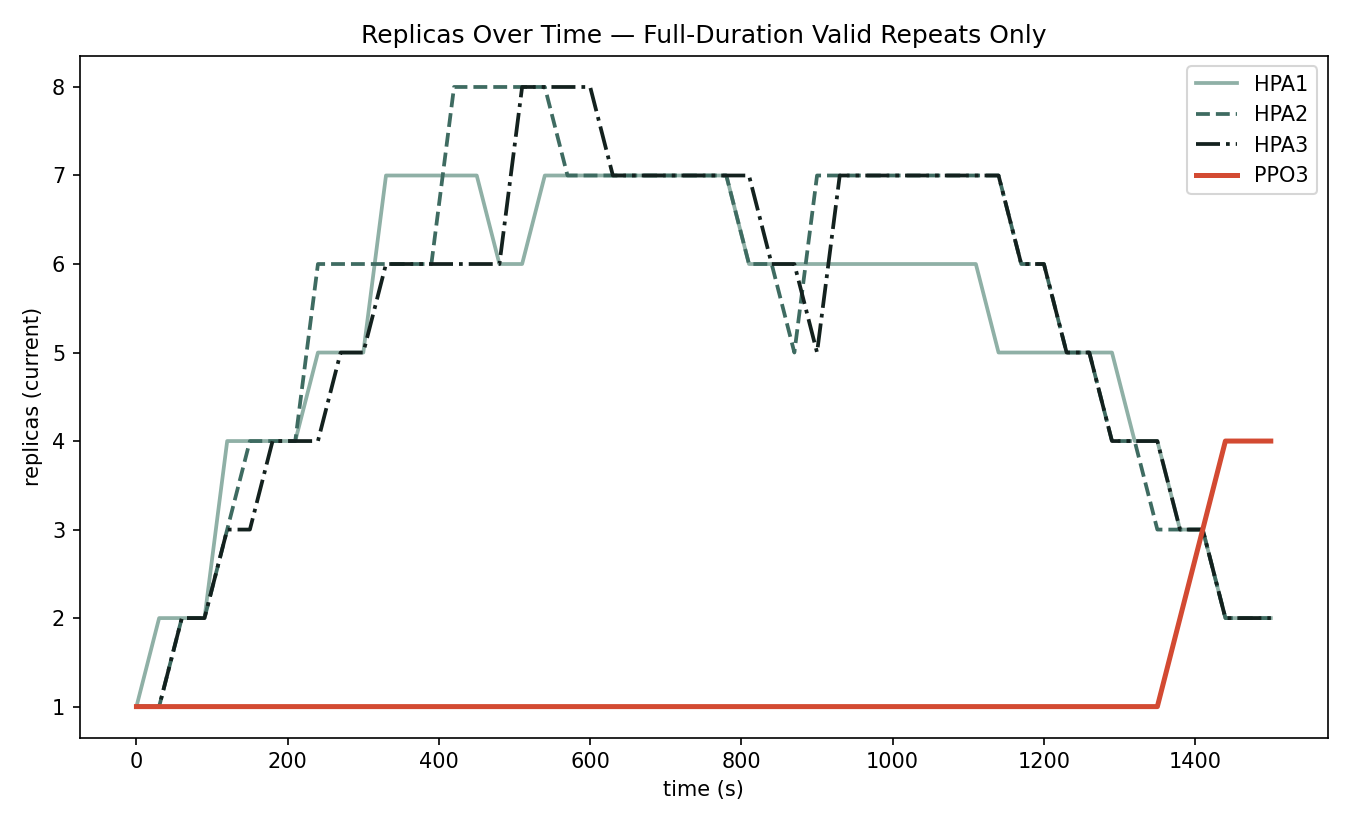
\includegraphics[width=0.42\textwidth]{../../results/figures/replicas_over_time_full_runs.png}
\caption{V1: replica count over time across the three full (non-terminated) runs of the held-out evaluation episode. Source: \texttt{results/\allowbreak \allowbreak figures/\allowbreak \allowbreak replicas\_\allowbreak over\_\allowbreak time\_\allowbreak full\_\allowbreak runs.png}.}
\label{fig:v1-replicas}
\end{figure}

\begin{figure}[htbp]
\centering
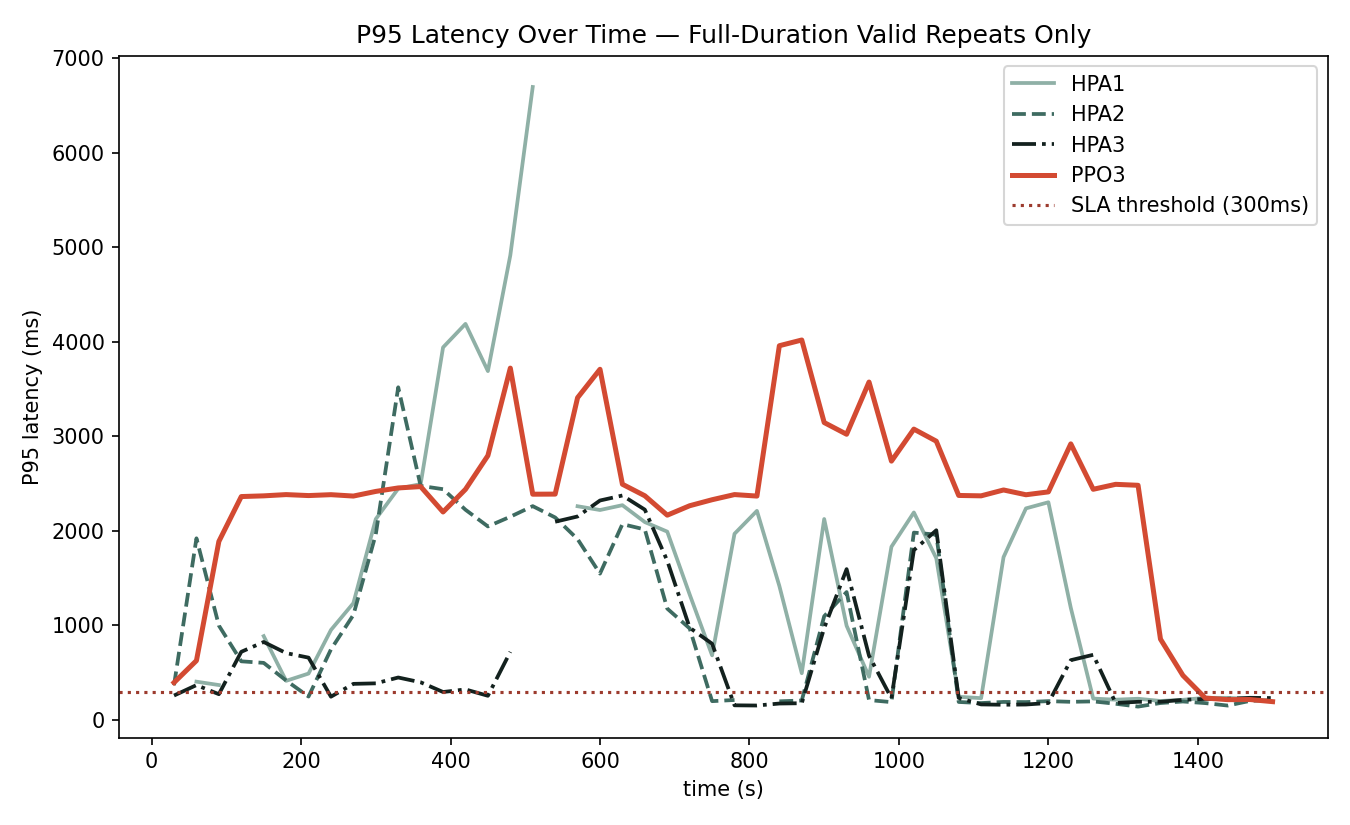
\includegraphics[width=0.42\textwidth]{../../results/figures/p95_latency_over_time_full_runs.png}
\caption{V1: p95 latency over time across the three full (non-terminated) runs of the held-out evaluation episode. Source: \texttt{results/\allowbreak \allowbreak figures/\allowbreak \allowbreak p95\_\allowbreak latency\_\allowbreak over\_\allowbreak time\_\allowbreak full\_\allowbreak runs.png}.}
\label{fig:v1-p95}
\end{figure}

\subsection{V1 Failure Analysis}
\label{sec:v1-failure}

Two of PPO's three evaluation runs (PPO1, PPO2) ended in a safety
termination triggered by \texttt{consecutive\_\allowbreak invalid\_\allowbreak steps\_\allowbreak limit\_\allowbreak reached}
roughly 10-11.5 minutes into their respective episodes, well after real
traffic had already been flowing continuously -- ruling out a one-off
cold-start telemetry gap as the explanation. We identified two design
decisions, both in V1 and both corrected in V2, that together explain this
pattern. First, V1's resource term in Equation~\ref{eq:v1-reward},
$-(n_t-1)/7$, charges a cost for every replica above one on every single
step, regardless of whether those replicas are doing anything useful; this
creates a persistent incentive to stay at the smallest possible replica
count even when load genuinely calls for more capacity. Second, V1's
replica floor of one meant that, once the policy had been driven toward a
single replica, that one pod's own saturation or a transient restart could
take the Deployment's entire ready-replica count to zero with no structural
redundancy to fall back on -- and a sustained loss of ready replicas is
exactly the condition that feeds \texttt{consecutive\_\allowbreak invalid\_\allowbreak steps}
toward its termination limit, since no telemetry can be attributed to a
pod that does not exist. A separate, SB3-default artefact compounds this:
deterministic inference's arg-max tie-break resolves an uncertain policy
toward the lowest action index, which in our action encoding is
\textsc{scale\_down\_one} -- so an uncertain V1 policy was silently biased
toward removing capacity even when it was not confidently the best choice,
never because removing capacity was actually assessed as correct. These
three findings -- an unconditional resource cost, a replica floor with no
redundancy, and a tie-break rule that silently favours scaling down -- are
precisely the three design points changed first in the V2 redesign of
Section~\ref{sec:v1-to-v2}.

\section{V2 Training Campaign}

\subsection{Learning Curves}

Figure~\ref{fig:training-reward} through Figure~\ref{fig:training-action-mix}
show the V2 training campaign's learning indicators across all 48 analyzed
sessions (12,288 cumulative timesteps). Dashed vertical markers in each
figure indicate sessions 4 and 38, the two sessions that failed and were
retried (Section~\ref{sec:zero-ready-stops}).

\begin{figure}[htbp]
\centering
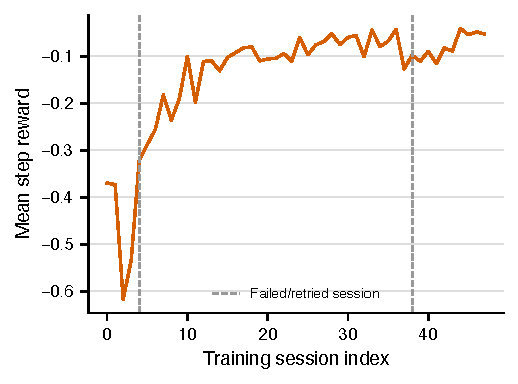
\includegraphics[width=0.42\textwidth]{../figures/training_mean_step_reward.pdf}
\caption{Mean per-step reward per training session, 48 sessions; dashed lines mark sessions 4 and 38 (failed, retried).}
\label{fig:training-reward}
\end{figure}

\begin{figure}[htbp]
\centering
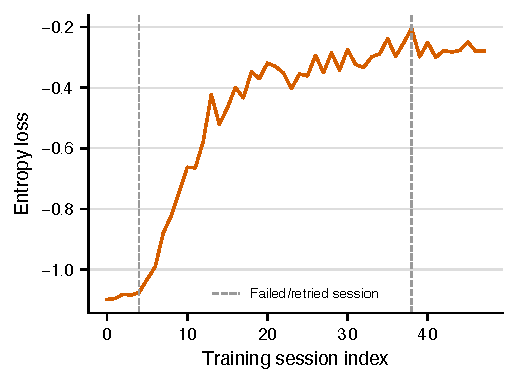
\includegraphics[width=0.42\textwidth]{../figures/training_entropy.pdf}
\caption{Policy entropy loss per training session, 48 sessions; dashed lines mark sessions 4 and 38.}
\label{fig:training-entropy}
\end{figure}

\begin{figure}[htbp]
\centering
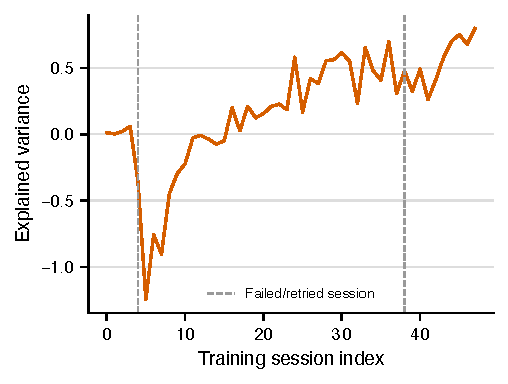
\includegraphics[width=0.42\textwidth]{../figures/training_explained_variance.pdf}
\caption{Explained variance of the value function per training session, 48 sessions; dashed lines mark sessions 4 and 38.}
\label{fig:training-ev}
\end{figure}

\begin{figure}[htbp]
\centering
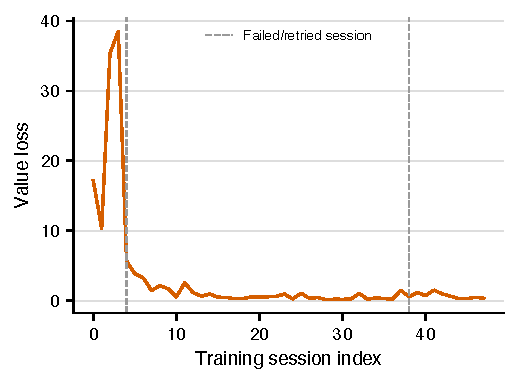
\includegraphics[width=0.42\textwidth]{../figures/training_value_loss.pdf}
\caption{Value loss per training session, 48 sessions; dashed lines mark sessions 4 and 38.}
\label{fig:training-vloss}
\end{figure}

\begin{figure}[htbp]
\centering
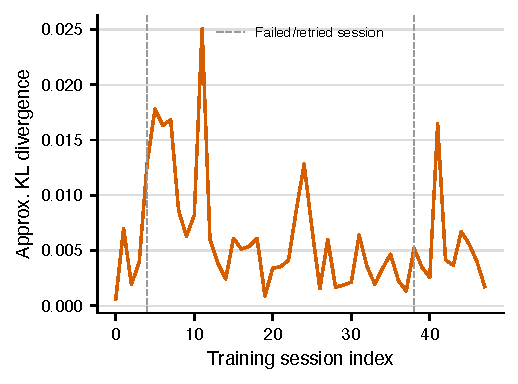
\includegraphics[width=0.42\textwidth]{../figures/training_approx_kl.pdf}
\caption{Approximate KL divergence per PPO update, 48 sessions; dashed lines mark sessions 4 and 38.}
\label{fig:training-kl}
\end{figure}

\begin{figure}[htbp]
\centering
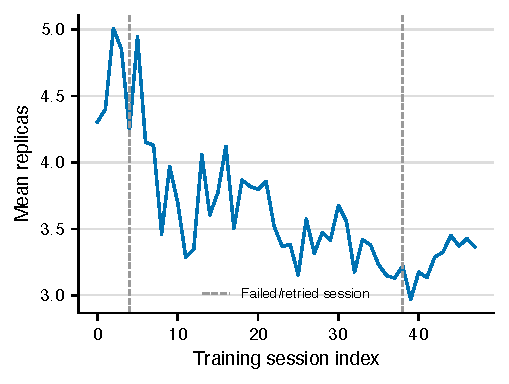
\includegraphics[width=0.42\textwidth]{../figures/training_mean_replicas.pdf}
\caption{Mean replica count per training session, 48 sessions; dashed lines mark sessions 4 and 38.}
\label{fig:training-replicas}
\end{figure}

\begin{figure}[htbp]
\centering
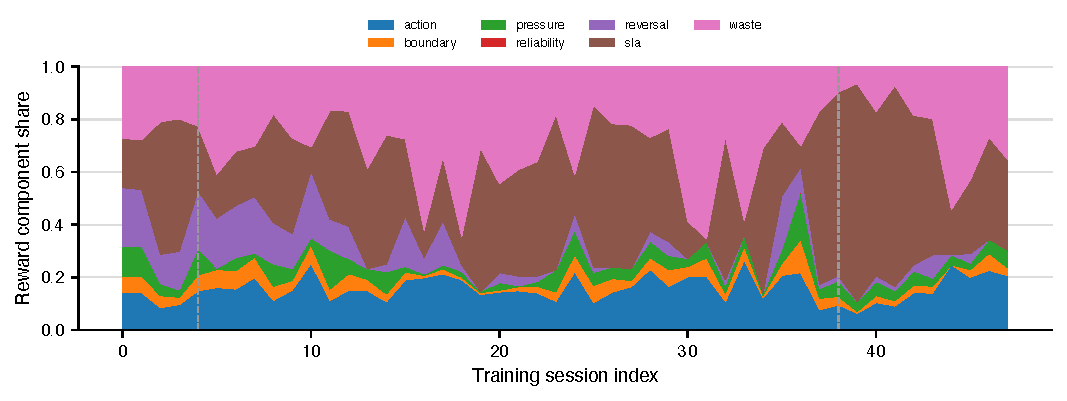
\includegraphics[width=0.42\textwidth]{../figures/training_reward_components.pdf}
\caption{Relative share of each reward component (by absolute mean value) per training session, 48 sessions; dashed lines mark sessions 4 and 38.}
\label{fig:training-components}
\end{figure}

\begin{figure}[htbp]
\centering
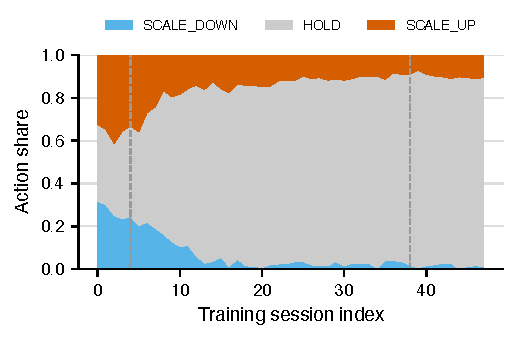
\includegraphics[width=0.42\textwidth]{../figures/training_action_mix.pdf}
\caption{Fraction of SCALE\_DOWN/HOLD/SCALE\_UP actions per training session, 48 sessions; dashed lines mark sessions 4 and 38.}
\label{fig:training-action-mix}
\end{figure}

Table~\ref{tab:training-summary} summarizes the key endpoints: entropy
loss, which measures how random the policy's action distribution is, falls
from $-1.0984$ at the first analyzed session to $-0.2792$ at the last,
consistent with the policy becoming progressively less random (more
confident in its choices) over the campaign. Explained variance of the
value function -- the fraction of the variance in observed returns that
the value function's predictions account for, with 1.0 meaning perfect
prediction and 0 meaning no better than predicting the mean -- rises from
0.0125 at the very first PPO update to a mean of 0.703 over the final five
updates (sessions 43-47), peaking at 0.799, computed directly from
\texttt{persistent-data/\allowbreak \allowbreak rl\_\allowbreak training\_\allowbreak v2/\allowbreak \allowbreak final\_\allowbreak min2/\allowbreak \allowbreak ppo\_\allowbreak update\_\allowbreak metrics.jsonl}.
This rise is not perfectly monotonic: the same underlying data shows a
minimum explained variance of $-1.2461$ at some point after the first
update (Table~\ref{tab:training-summary}), meaning the value function's
predictions were, briefly, worse than simply predicting the mean return --
consistent with PPO's on-policy updates occasionally destabilizing the
value function's fit before it recovers, which is a known and generally
tolerated property of on-policy actor-critic training rather than a sign
that training failed.

\begin{table}[H]
\centering
\caption{V2 training summary: key endpoints across 48 analyzed sessions.}
\label{tab:training-summary}
\begin{tabular}{ll}
\hline
field & value \\
\hline
n\_sessions\_analyzed & 48 \\
first\_session\_entropy\_loss & -1.0984 \\
last\_session\_entropy\_loss & -0.2792 \\
min\_entropy\_loss & -1.0984 \\
max\_entropy\_loss & -0.2048 \\
first\_session\_explained\_variance & 0.0125 \\
last\_session\_explained\_variance & 0.7993 \\
min\_explained\_variance & -1.2461 \\
max\_explained\_variance & 0.7993 \\
n\_failed\_retried\_attempts & 2 \\
failed\_attempt\_session\_indices & 4, 38 \\
\hline
\end{tabular}

\end{table}

\subsection{Training Progression}

Reading the same underlying curves as a progression rather than only as
endpoints: mean step reward improves steadily across the campaign, the
HOLD action's share of all decisions rises as the policy learns to avoid
unnecessary scaling churn, and mean replica count drifts downward from an
early-campaign level toward the lower half of the 2-8 replica range,
consistent with the policy learning that most of the training traffic
profiles do not need many replicas to keep latency and error rate healthy.
This progression is visible directly in
Figures~\ref{fig:training-reward}-\ref{fig:training-action-mix} and is the
basis for the discussion of what the policy had and had not converged to
by session 47 in Section~\ref{sec:discussion}.

\subsection{The Two Zero-Ready-Pod Stops}
\label{sec:zero-ready-stops}

Two of the campaign's 48 planned sessions failed on their first physical
attempt and had to be resumed from the previous checkpoint: session 4 and
session 38. Both failures share the identical recorded reason,
\texttt{zero\_\allowbreak ready\_\allowbreak replicas}, read directly from each session's own
\texttt{SESSION\_\allowbreak FAILED.json}: session 4 failed after completing 126 of
its planned 256 steps, and session 38 after completing 163 of 256. In both
cases, every ready replica of the Deployment dropped to zero during the
session -- the same structural failure mode diagnosed for V1 in
Section~\ref{sec:v1-failure}, except that by this point in the V2 campaign
the replica floor had already been raised to 2 (CORR-55), so this is not a
recurrence of the single-replica vulnerability itself; it reflects that a
floor of 2 reduces, but does not eliminate, the chance that correlated pod
unhealthiness (for example, both replicas restarting close together under
load) can still, on rare occasions, take ready-replica count to zero. Both
sessions were resumed from their last good checkpoint using the
session/checkpoint/resume design of Chapter~\ref{ch:methodology}, each
completing successfully as session \texttt{\_\allowbreak \_\allowbreak attempt2}, which is why the
campaign's 48 analyzed sessions are complete, successful retries and not a
silently dropped or averaged-over set of failures; both are marked
explicitly with dashed lines in every learning-curve figure in this
section.

A closely related event, worth reporting plainly rather than omitting, is
documented in the project's own Phase 5E report: partway through an
unrelated, offline user-interface development task, a routine, read-only
process check found that the live training campaign's process (PID 26490)
had disappeared. Reading the campaign's own metadata file showed the
campaign had stopped itself at session 4 on the \texttt{zero\_\allowbreak ready\_\allowbreak replicas}
condition described above, with sessions 0-3 already safely checkpointed;
no command from that phase, or any other phase, had touched the cluster,
the lock file, or the training process at any point, and the project's own
established discipline was followed: no restart or retry was attempted
until the stoppage had been reviewed. \textbf{[CHECK]}: our search of this
project's documentation did not turn up a separately confirmed incident in
which the V2 training process itself was killed by an external signal
(as distinct from the self-terminating \texttt{zero\_\allowbreak ready\_\allowbreak replicas}
stops at sessions 4 and 38 described above); if such an externally-killed
re-run occurred, we were not able to locate its record in the materials
available to us and flag this explicitly rather than asserting a cause we
could not verify.

\section{Pre-Registered Evaluation}

\subsection{Overview}

The pre-registered \texttt{eval\_\allowbreak final} campaign (CORR-60) ran all 27
planned attempts (3 profiles $\times$ 3 arms $\times$ 3 repeats) to a
VALID outcome. No run ended in a safety termination; no pod restarted
during any of the 27 runs (\texttt{pod\_\allowbreak restarts\_\allowbreak total == 0} throughout).
Four attempts failed on their first try due to a leftover HPA object from
the previous arm's run blocking controller acquisition (CORR-63, CORR-64)
and were retried once each under the tooling-failure rule of
Section~\ref{sec:eval-protocol}, with zero effect on the measured result
once retried; this is reported here rather than silently absorbed into the
27 VALID figures, consistent with this project's discipline of preserving
every attempt's evidence, successful or not.

\subsection{Primary Metrics}

Table~\ref{tab:eval-primary} reports the primary metrics, mean $\pm$
standard deviation over the three repeats of each (profile, arm) cell.

\begin{table}[H]
\centering
\caption{\texttt{eval\_\allowbreak final} primary metrics: SLA-violation rate at the 1000\,ms target and replica-minutes, mean $\pm$ sd over 3 repeats.}
\label{tab:eval-primary}
\small
\resizebox{\linewidth}{!}{\begin{tabular}{lllll}
\hline
profile & arm & n\_repeats & sla\_violation\_rate\_1000ms & replica\_minutes \\
\hline
CPU step & HPA CPU+Memory (resource baseline) & 3 & 0.0000 +/- 0.0000 & 60.5000 +/- 0.8660 \\
CPU step & HPA CPU-only (CPU baseline) & 3 & 0.0000 +/- 0.0000 & 59.3333 +/- 0.2887 \\
CPU step & PPO (multi-metric, 11 signals) & 3 & 0.0083 +/- 0.0144 & 72.6667 +/- 0.2887 \\
memory ramp & HPA CPU+Memory (resource baseline) & 3 & 0.0000 +/- 0.0000 & 75.1667 +/- 1.6073 \\
memory ramp & HPA CPU-only (CPU baseline) & 3 & 0.0000 +/- 0.0000 & 40.0000 +/- 0.0000 \\
memory ramp & PPO (multi-metric, 11 signals) & 3 & 0.0000 +/- 0.0000 & 56.1667 +/- 0.2887 \\
mixed bursts & HPA CPU+Memory (resource baseline) & 3 & 0.0000 +/- 0.0000 & 74.6667 +/- 5.1316 \\
mixed bursts & HPA CPU-only (CPU baseline) & 3 & 0.0000 +/- 0.0000 & 40.0000 +/- 0.0000 \\
mixed bursts & PPO (multi-metric, 11 signals) & 3 & 0.0000 +/- 0.0000 & 58.3333 +/- 2.3094 \\
\hline
\end{tabular}
}
\end{table}

Under our pre-registered decision rule (Table~\ref{tab:decision-rule}: an
arm is "better" on a metric for a profile only if it wins in all three of
three repeats), the SLA-violation rate at the 1000\,ms target does not
produce a decidable winner for any arm pair on any profile -- every arm
sits at or extremely close to its floor of 0.0 on every profile, with the
one exception of PPO on \texttt{eval\_\allowbreak cpu\_\allowbreak step} (mean 0.0083, i.e.\ a
single decision out of 360 total PPO decisions breached the SLA across the
whole campaign), which is itself too close to zero, and too inconsistent
across repeats ($\pm 0.0144$), to support a "better" claim either way.
Replica-minutes (our cost proxy) does discriminate, but not in favour of a
single arm: the HPA CPU-only (CPU baseline) arm is cheapest on
\texttt{eval\_\allowbreak memory\_\allowbreak ramp} (40.0 versus PPO's 56.17 and the HPA
CPU+Memory arm's 75.17) and on \texttt{eval\_\allowbreak mixed\_\allowbreak burst} (40.0 versus
58.33 and 74.67), and effectively ties with HPA CPU+Memory on
\texttt{eval\_\allowbreak cpu\_\allowbreak step} (59.33 versus 60.5, both cheaper than PPO's
72.67). PPO is therefore the most expensive arm on \texttt{eval\_\allowbreak cpu\_\allowbreak step}
but the cheapest of the three arms on the other two profiles besides the
CPU-only baseline -- a profile-dependent cost ranking, not a uniform one,
exactly the kind of outcome our decision rule is built to report as a
trade-off rather than resolve into a single ranking.

\subsection{Secondary Metrics}

Table~\ref{tab:eval-secondary-main} reports mean p95 latency and maximum
per-pod memory for each cell; the full secondary-metrics table, including
error rate, scaling-action and reversal counts, and the 300\,ms reference
SLA rate, is given in Appendix~\ref{ch:appendix},
Table~\ref{tab:eval-secondary-appendix}.

\begin{table}[H]
\centering
\caption{\texttt{eval\_\allowbreak final} secondary metrics (selected columns): mean p95 latency and maximum per-pod memory, mean $\pm$ sd over 3 repeats.}
\label{tab:eval-secondary-main}
\small
\begin{tabular}{llrr}
\toprule
Profile & Arm & Mean p95 (ms) & Max per-pod memory (MiB) \\
\midrule
eval\_cpu\_step & HPA CPU+Memory & $270.9 \pm 36.3$ & $48.5 \pm 9.6$ \\
eval\_cpu\_step & HPA CPU-only & $249.7 \pm 4.1$ & $56.8 \pm 3.9$ \\
eval\_cpu\_step & PPO & $274.1 \pm 92.6$ & $51.6 \pm 10.3$ \\
eval\_memory\_ramp & HPA CPU+Memory & $975.0 \pm 0.0$ & $123.8 \pm 10.8$ \\
eval\_memory\_ramp & HPA CPU-only & $975.0 \pm 0.0$ & $140.9 \pm 9.0$ \\
eval\_memory\_ramp & PPO & $950.6 \pm 0.0$ & $108.6 \pm 9.5$ \\
eval\_mixed\_burst & HPA CPU+Memory & $975.0 \pm 0.0$ & $97.6 \pm 18.4$ \\
eval\_mixed\_burst & HPA CPU-only & $975.1 \pm 0.1$ & $119.0 \pm 0.2$ \\
eval\_mixed\_burst & PPO & $950.6 \pm 0.0$ & $108.2 \pm 9.0$ \\
\bottomrule
\end{tabular}
\end{table}

The recurring value of exactly 975\,ms on the memory and mixed profiles,
for every arm, is a Prometheus histogram-bucket interpolation artefact,
not a precisely measured latency: our latency histogram's bucket
boundaries mean that a true p95 anywhere between 500\,ms and 1,000\,ms can
be reported back as 975\,ms. We flag this plainly rather than treating it
as a precise measurement, and it is the direct motivation for raising the
V2 SLA target from 300\,ms to 1,000\,ms (CORR-57) described in
Section~\ref{sec:v1-to-v2}.

\subsection{Workload and Latency Figures}

Figure~\ref{fig:workloads} shows the request-rate shape of the three
\texttt{eval\_\allowbreak final} profiles. Figures~\ref{fig:eval-box-cpu}-\ref{fig:eval-box-mixed}
show box plots of per-decision p95 latency, pooled across the three
repeats of each profile; \textbf{these box plots use a symmetric-log
(symlog) vertical axis} (linear threshold 200\,ms, switching to
logarithmic scaling beyond it) because a linear axis compresses every box
into an unreadably thin line at this project's latency scale, and this is
stated explicitly in each figure's caption as required.

\begin{figure}[htbp]
\centering
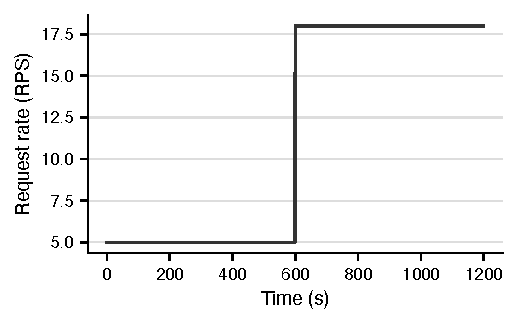
\includegraphics[width=0.32\textwidth]{../figures/workloads_eval_cpu_step.pdf}
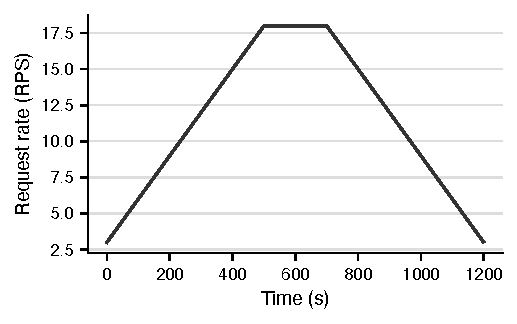
\includegraphics[width=0.32\textwidth]{../figures/workloads_eval_memory_ramp.pdf}
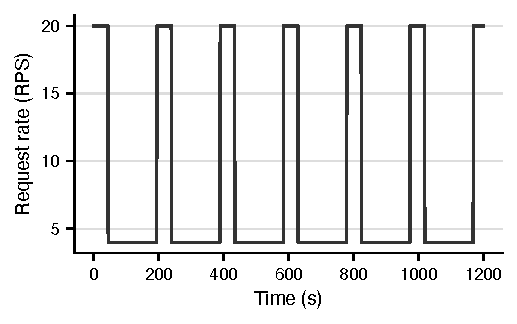
\includegraphics[width=0.32\textwidth]{../figures/workloads_eval_mixed_burst.pdf}
\caption{Request rate (RPS) versus time for the three pre-registered \texttt{eval\_\allowbreak final} profiles: \texttt{eval\_\allowbreak cpu\_\allowbreak step} (peak 18 RPS, CPU mode), \texttt{eval\_\allowbreak memory\_\allowbreak ramp} (peak 18 RPS, memory mode), \texttt{eval\_\allowbreak mixed\_\allowbreak burst} (peak 20 RPS, mixed mode).}
\label{fig:workloads}
\end{figure}

\begin{figure}[htbp]
\centering
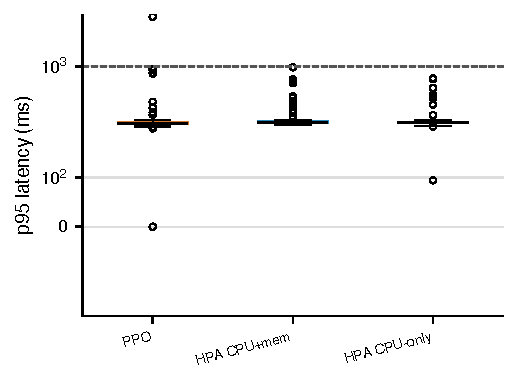
\includegraphics[width=0.42\textwidth]{../figures/evaluation_p95_boxplot_eval_cpu_step.pdf}
\caption{Box plot (symlog vertical axis, linear threshold 200\,ms) of per-decision p95 latency, pooled across 3 repeats, \texttt{eval\_\allowbreak cpu\_\allowbreak step}. Dashed line: 1000\,ms SLA target.}
\label{fig:eval-box-cpu}
\end{figure}

\begin{figure}[htbp]
\centering
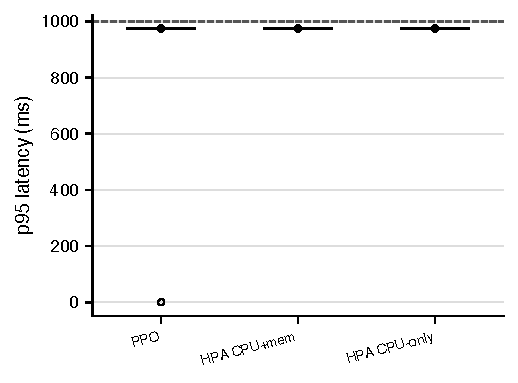
\includegraphics[width=0.42\textwidth]{../figures/evaluation_p95_boxplot_eval_memory_ramp.pdf}
\caption{Box plot (symlog vertical axis, linear threshold 200\,ms) of per-decision p95 latency, pooled across 3 repeats, \texttt{eval\_\allowbreak memory\_\allowbreak ramp}. Dashed line: 1000\,ms SLA target. The 975\,ms cluster is the histogram-bucket artefact described in the text.}
\label{fig:eval-box-memory}
\end{figure}

\begin{figure}[htbp]
\centering
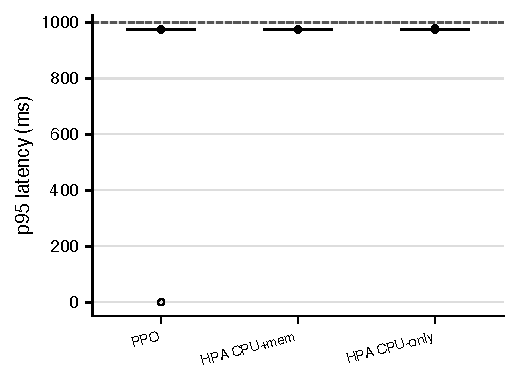
\includegraphics[width=0.42\textwidth]{../figures/evaluation_p95_boxplot_eval_mixed_burst.pdf}
\caption{Box plot (symlog vertical axis, linear threshold 200\,ms) of per-decision p95 latency, pooled across 3 repeats, \texttt{eval\_\allowbreak mixed\_\allowbreak burst}. Dashed line: 1000\,ms SLA target. The 975\,ms cluster is the histogram-bucket artefact described in the text.}
\label{fig:eval-box-mixed}
\end{figure}

Figure~\ref{fig:eval-replica-minutes} shows replica-minutes per profile
and arm with error bars (mean $\pm$ sd), and
Figures~\ref{fig:eval-replicas-cpu}-\ref{fig:eval-p95-mixed} show replica
count and p95 latency over time for the median-cost repeat of each arm on
each profile.

\begin{figure}[htbp]
\centering
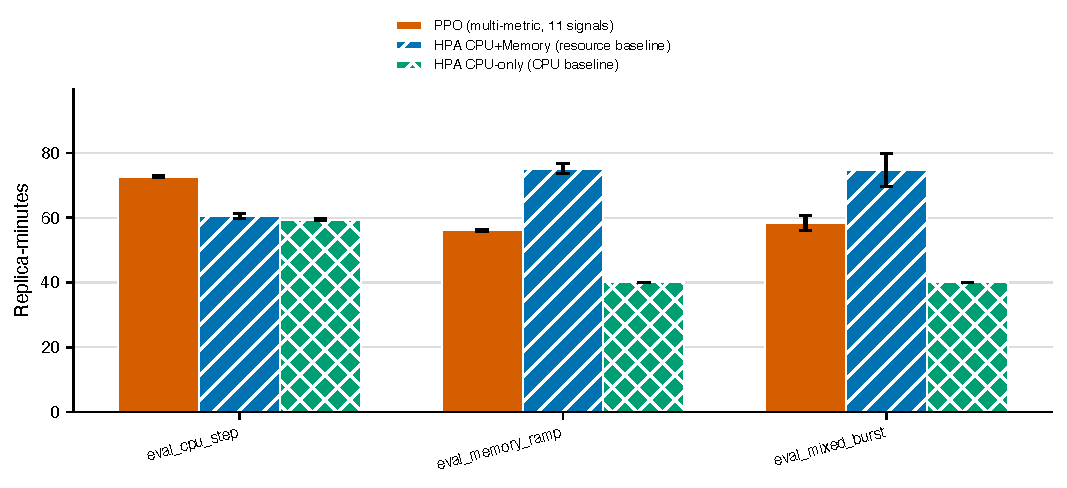
\includegraphics[width=0.42\textwidth]{../figures/evaluation_replica_minutes.pdf}
\caption{Replica-minutes (cost proxy), mean $\pm$ sd over 3 repeats, per profile and arm, \texttt{eval\_\allowbreak final}.}
\label{fig:eval-replica-minutes}
\end{figure}

\begin{figure}[htbp]
\centering
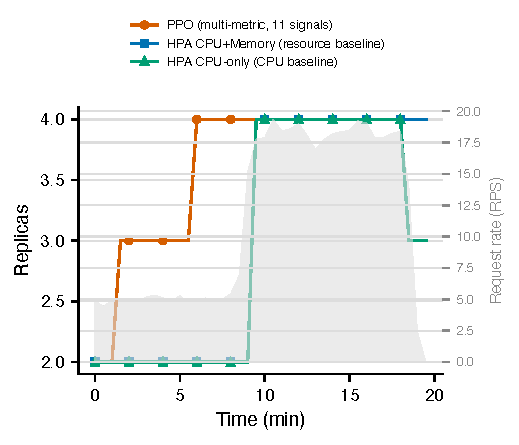
\includegraphics[width=0.42\textwidth]{../figures/evaluation_replicas_over_time_eval_cpu_step.pdf}
\caption{Replica count over time, \texttt{eval\_\allowbreak cpu\_\allowbreak step}, all 3 arms (median-cost repeat per arm), with request rate as a light background.}
\label{fig:eval-replicas-cpu}
\end{figure}

\begin{figure}[htbp]
\centering
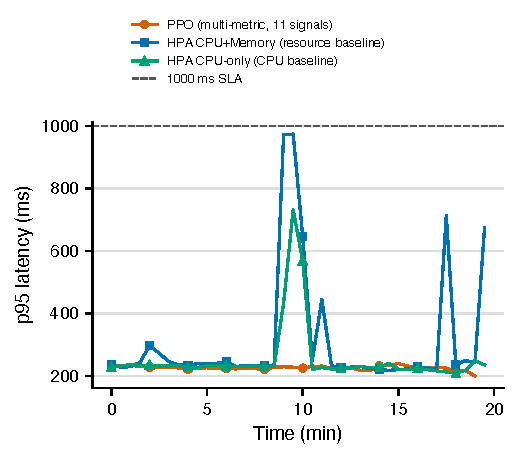
\includegraphics[width=0.42\textwidth]{../figures/evaluation_p95_over_time_eval_cpu_step.pdf}
\caption{p95 latency over time, \texttt{eval\_\allowbreak cpu\_\allowbreak step}, all 3 arms (median-cost repeat per arm), with the 1000\,ms SLA line.}
\label{fig:eval-p95-cpu}
\end{figure}

\begin{figure}[htbp]
\centering
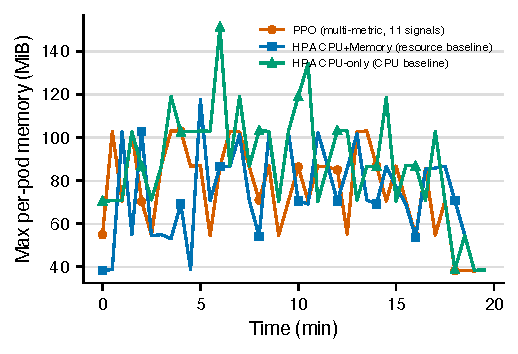
\includegraphics[width=0.42\textwidth]{../figures/evaluation_memory_over_time.pdf}
\caption{Maximum per-pod memory (MiB) over time on \texttt{eval\_\allowbreak memory\_\allowbreak ramp}, all 3 arms (median-cost repeat per arm).}
\label{fig:eval-memory-time}
\end{figure}

\begin{figure}[htbp]
\centering
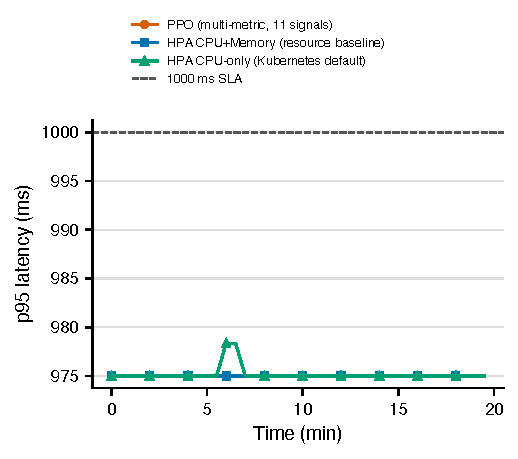
\includegraphics[width=0.42\textwidth]{../figures/evaluation_p95_over_time_eval_mixed_burst.pdf}
\caption{p95 latency over time, \texttt{eval\_\allowbreak mixed\_\allowbreak burst}, all 3 arms (median-cost repeat per arm), with the 1000\,ms SLA line.}
\label{fig:eval-p95-mixed}
\end{figure}

\subsection{PPO Policy Behaviour and Tie-Break Usage}

Across all 360 PPO decisions made during \texttt{eval\_\allowbreak final} (27 PPO
episodes $\times$ 40 decisions each, for the 9 PPO runs), HOLD was chosen
347 times, SCALE\_UP\_ONE 13 times (3.6\%), and SCALE\_DOWN\_ONE never.
Figure~\ref{fig:ppo-policy-map} shows the dominant action per
(CPU-per-replica, memory-per-replica) bin: HOLD dominates almost every
bin, and the 13 scale-up decisions are spread across a wide range of CPU
values rather than concentrated only at high CPU, suggesting the policy's
scale-up decisions are driven by more than CPU alone, consistent with its
eleven-feature, multi-signal observation space.

\begin{figure}[htbp]
\centering
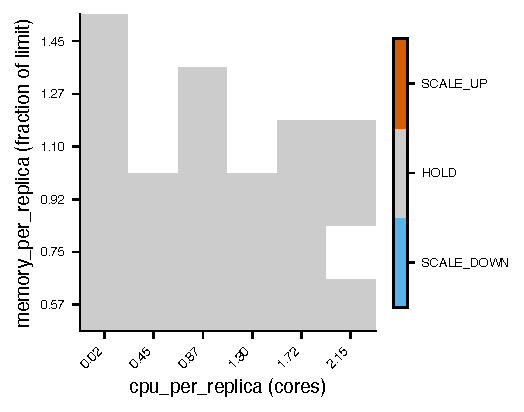
\includegraphics[width=0.42\textwidth]{../figures/discussion_ppo_policy_map.pdf}
\caption{Dominant action (SCALE\_DOWN/HOLD/SCALE\_UP) per (CPU-per-replica, memory-per-replica) bin, \texttt{eval\_\allowbreak final} PPO decisions. HOLD dominates almost every bin; only 13 of 360 decisions (3.6\%) are SCALE\_UP.}
\label{fig:ppo-policy-map}
\end{figure}

The safety-aware tie-break rule of Section~\ref{sec:tie-break} fired (that
is, an actual tie among two or more actions was detected and resolved by
rules R3-R6, not simply R1's "no tie") in exactly 4 of these 360 decisions
(1.11\%), shown in Figure~\ref{fig:tie-rule-frequency}. The rule is, by
design and in practice, a rare intervention: the overwhelming majority of
decisions have a single clear highest-probability action, and the rule
only matters at the margin.

\begin{figure}[htbp]
\centering
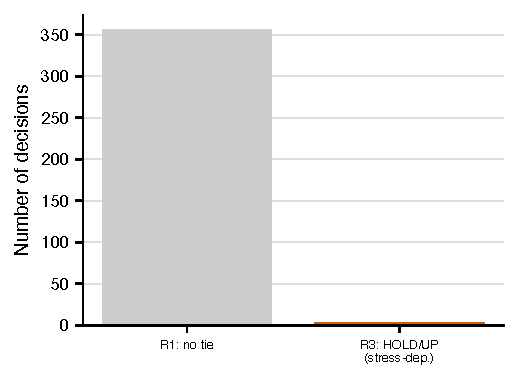
\includegraphics[width=0.42\textwidth]{../figures/discussion_tie_rule_frequency.pdf}
\caption{Frequency of each CORR-58 tie-break rule firing across \texttt{eval\_\allowbreak final} PPO decisions (R1 = no tie; R3-R6 = an actual tie resolved). An actual tie-break fired in 4 of 360 decisions (1.11\%).}
\label{fig:tie-rule-frequency}
\end{figure}

\subsection{Verdict}

Applying the pre-registered decision rule of Table~\ref{tab:decision-rule}
to the results above: the SLA-violation-rate metric produces no decidable
winner between any pair of arms on any profile, because every arm sits at
or effectively at its floor of 0.0 at this evaluation's load levels. The
replica-minutes metric does discriminate, but not in a single arm's
favour across all three profiles: the HPA CPU-only (CPU baseline) arm is
cheapest on two of three profiles and ties on the third; PPO's cost
ranking is profile-dependent, cheaper than the HPA CPU+Memory arm on two
profiles but more expensive than both HPA arms on \texttt{eval\_\allowbreak cpu\_\allowbreak step}.
No safety termination occurred in any of the 27 valid runs. Per the
pre-registration's own rule against declaring a single aggregate winner
when metrics disagree, we report this explicitly as a profile-dependent
trade-off: \textbf{no controller is declared better than the others
overall}, and the latency objective, at these evaluation-level loads,
simply does not separate the three arms.

\section{Exploratory Stress Test}

\subsection{Overview}

The exploratory \texttt{stress\_\allowbreak explore} campaign (CORR-65) was added
after \texttt{eval\_\allowbreak final}'s results already existed, specifically because
those results showed the primary SLA metric sitting at or near its floor
for every arm, unable to discriminate between controllers at
\texttt{eval\_\allowbreak final}'s light load levels. Because this addition is
explicitly outcome-aware (it was motivated by having already seen
\texttt{eval\_\allowbreak final}'s results), it is run with only one repeat per
(profile, arm) cell (9 runs total, referencing the same three profiles'
training-level-peak counterparts: \texttt{stress\_\allowbreak cpu\_\allowbreak burst},
\texttt{stress\_\allowbreak memory\_\allowbreak ramp}, \texttt{stress\_\allowbreak mixed\_\allowbreak burst}, peaking at
45-70 RPS, never beyond loads already exercised live during training) and
is reported throughout as \textbf{descriptive only}: the pre-registered
"better in all 3 repeats" decision rule cannot be and is not applied to a
single-repeat dataset, and every figure and table from this campaign is
labelled exploratory so it can never be mistaken for, or merged with, the
pre-registered \texttt{eval\_\allowbreak final} results above.

\begin{figure}[htbp]
\centering
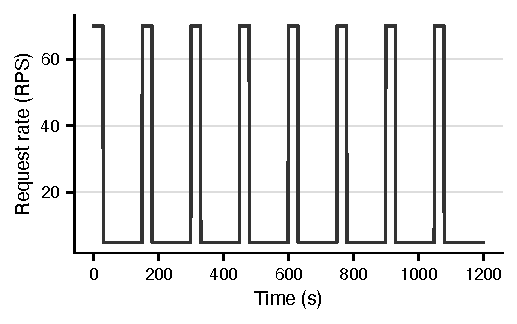
\includegraphics[width=0.32\textwidth]{../figures/workloads_stress_cpu_burst.pdf}
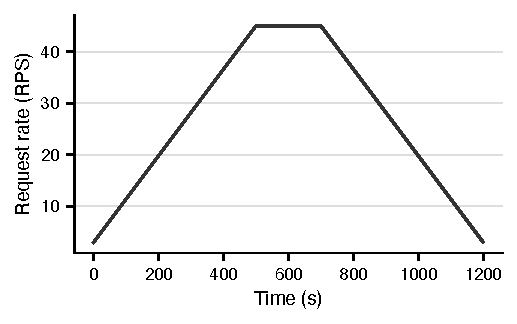
\includegraphics[width=0.32\textwidth]{../figures/workloads_stress_memory_ramp.pdf}
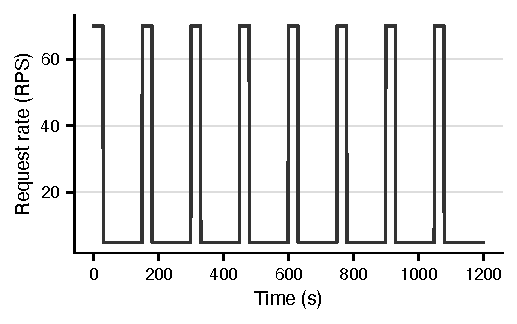
\includegraphics[width=0.32\textwidth]{../figures/workloads_stress_mixed_burst.pdf}
\caption{Request rate (RPS) versus time for the three exploratory \texttt{stress\_\allowbreak explore} profiles (CORR-65): \texttt{stress\_\allowbreak cpu\_\allowbreak burst} (peak 70 RPS), \texttt{stress\_\allowbreak memory\_\allowbreak ramp} (peak 45 RPS), \texttt{stress\_\allowbreak mixed\_\allowbreak burst} (peak 70 RPS).}
\label{fig:workloads-stress}
\end{figure}

\subsection{Descriptive Results}

Table~\ref{tab:stress-descriptive-main} reports the primary descriptive
metrics for all 9 stress runs (1 repeat each); the full table, including
secondary metrics, is given in Appendix~\ref{ch:appendix},
Table~\ref{tab:stress-descriptive-appendix}.

\begin{table}[H]
\centering
\caption{\texttt{stress\_\allowbreak explore} descriptive metrics (selected columns), 1 repeat per cell -- exploratory, CORR-65.}
\label{tab:stress-descriptive-main}
\small
\begin{tabular}{llrrr}
\toprule
Profile & Arm & SLA-viol.\ (1000\,ms) & Replica-minutes & Mean p95 (ms) \\
\midrule
stress\_cpu\_burst & HPA CPU+Memory & 0.5263 & 123.00 & 1820.3 \\
stress\_cpu\_burst & HPA CPU-only & 0.5250 & 130.00 & 1703.1 \\
stress\_cpu\_burst & PPO & 0.5000 & 84.00 & 1567.6 \\
stress\_memory\_ramp & HPA CPU+Memory & 0.0000 & 78.00 & 975.0 \\
stress\_memory\_ramp & HPA CPU-only & 0.0000 & 40.00 & 975.0 \\
stress\_memory\_ramp & PPO & 0.0000 & 56.00 & 950.6 \\
stress\_mixed\_burst & HPA CPU+Memory & 0.0000 & 76.00 & 980.3 \\
stress\_mixed\_burst & HPA CPU-only & 0.1000 & 62.50 & 1041.4 \\
stress\_mixed\_burst & PPO & 0.2000 & 66.50 & 1091.7 \\
\bottomrule
\end{tabular}
\end{table}

Under \texttt{stress\_\allowbreak cpu\_\allowbreak burst}, all three arms miss the SLA objective
roughly half the time (0.50-0.53), with PPO lowest on both cost (84.0
replica-minutes versus 123.0-130.0 for the two HPA arms) and mean p95
latency (1567.6\,ms versus 1703.1-1820.3\,ms); Figure~\ref{fig:stress-replicas-cpu}
shows why: both HPA arms repeatedly hit the 8-replica ceiling under this
profile, while PPO rises step by step to 5 replicas and holds there,
spending less on replicas while still achieving slightly lower latency.
Under \texttt{stress\_\allowbreak memory\_\allowbreak ramp}, no arm breaches the SLA at all, and
PPO's cost (56.0) sits between the HPA CPU-only arm's 40.0 and the HPA
CPU+Memory arm's 78.0. Under \texttt{stress\_\allowbreak mixed\_\allowbreak burst}, the ordering
reverses: PPO has the \emph{highest} SLA-violation rate of the three arms
(0.20, versus 0.00 for HPA CPU+Memory and 0.10 for HPA CPU-only) at a
mid-range cost (66.5) -- the opposite ordering from
\texttt{stress\_\allowbreak cpu\_\allowbreak burst}. \textbf{No single arm is uniformly better
across all three stress profiles.}

\begin{figure}[htbp]
\centering
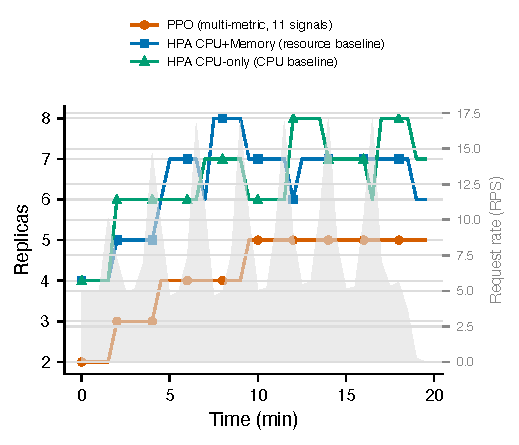
\includegraphics[width=0.42\textwidth]{../figures/stress_replicas_over_time_stress_cpu_burst.pdf}
\caption{Replica count over time, \texttt{stress\_\allowbreak cpu\_\allowbreak burst} (exploratory, CORR-65, 1 repeat per arm), with request rate as a light background. Both HPA arms repeatedly hit the 8-replica ceiling; PPO caps at 5 replicas.}
\label{fig:stress-replicas-cpu}
\end{figure}

\begin{figure}[htbp]
\centering
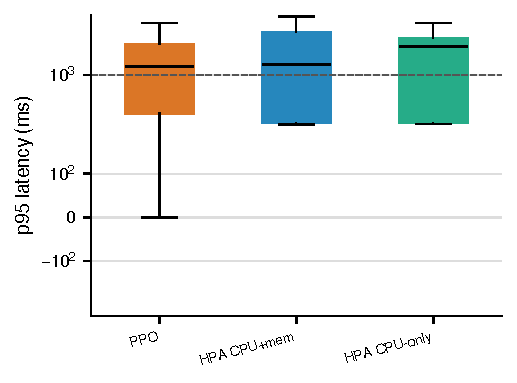
\includegraphics[width=0.42\textwidth]{../figures/stress_p95_boxplot_stress_cpu_burst.pdf}
\caption{Box plot (symlog vertical axis, linear threshold 200\,ms) of per-decision p95 latency, \texttt{stress\_\allowbreak cpu\_\allowbreak burst} (exploratory, CORR-65, 1 repeat per arm). Dashed line: 1000\,ms SLA target.}
\label{fig:stress-box-cpu}
\end{figure}

\begin{figure}[htbp]
\centering
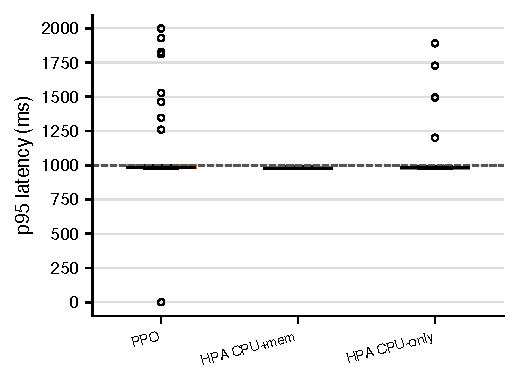
\includegraphics[width=0.42\textwidth]{../figures/stress_p95_boxplot_stress_mixed_burst.pdf}
\caption{Box plot (symlog vertical axis, linear threshold 200\,ms) of per-decision p95 latency, \texttt{stress\_\allowbreak mixed\_\allowbreak burst} (exploratory, CORR-65, 1 repeat per arm). Dashed line: 1000\,ms SLA target. PPO shows a wider spread above the SLA line than either HPA arm here, consistent with its higher SLA-violation rate on this profile.}
\label{fig:stress-box-mixed}
\end{figure}

\begin{figure}[htbp]
\centering
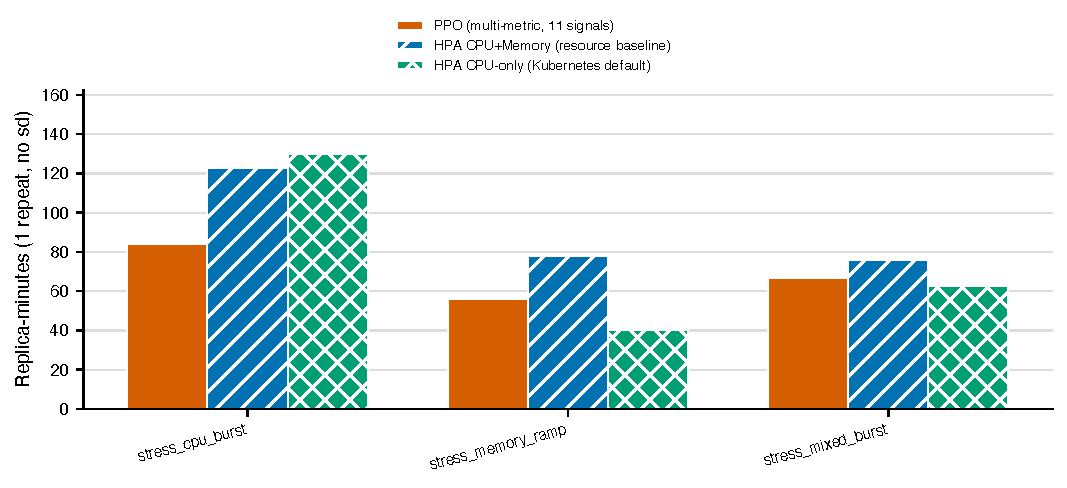
\includegraphics[width=0.42\textwidth]{../figures/stress_replica_minutes.pdf}
\caption{Replica-minutes (cost proxy), 1 repeat per cell (no error bars), per profile and arm, \texttt{stress\_\allowbreak explore} (exploratory, CORR-65).}
\label{fig:stress-replica-minutes}
\end{figure}

Figure~\ref{fig:cost-vs-latency} places every run from both campaigns on a
single cost-versus-latency plot: the exploratory stress-test points sit
well above and to the right of the \texttt{eval\_\allowbreak final} cluster, showing
that both cost and latency rise together once load moves from
\texttt{eval\_\allowbreak final}'s light levels to training-level peaks.

\begin{figure}[htbp]
\centering
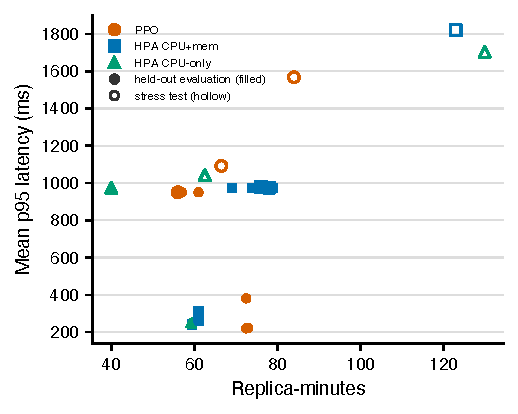
\includegraphics[width=0.42\textwidth]{../figures/discussion_cost_vs_latency.pdf}
\caption{Replica-minutes (x-axis) versus mean p95 latency (y-axis), one point per run; \texttt{eval\_\allowbreak final} points filled, \texttt{stress\_\allowbreak explore} points hollow.}
\label{fig:cost-vs-latency}
\end{figure}

\section{Comparative Analysis Against Related Work}
\label{sec:comparative-analysis}

Returning to Table~\ref{tab:related-work-summary} in
Chapter~\ref{ch:introduction}: the studies we surveyed that report
favourable RL-versus-baseline comparisons (Mao et al.\
\cite{mao2016resource}, Rossi et al.\ \cite{rossi2019horizontal}, Imdoukh
et al.\ \cite{imdoukh2020lstm}, Qiu et al.\ \cite{qiu2020firm}) train
and/or evaluate primarily in a simulator or against a recorded trace, and,
as far as we could establish from their published descriptions, do not
report a baseline comparison whose protocol and decision rule were fixed
in writing before any evaluation result existed. Our project differs on
both counts: every decision step, in both V1 and V2, training and
evaluation, was executed against a real Minikube cluster, and our V2
evaluation protocol, metrics, and decision rule were pre-registered
(CORR-60) before the final training checkpoint existed. This difference
has a direct, visible cost: our sample sizes (three repeats per
pre-registered cell, one per exploratory cell) are far smaller than a
simulator-based study could collect in the same wall-clock time, and our
results are correspondingly more cautious -- we report a profile-dependent
trade-off rather than a clean win, where some of the surveyed simulator-
or trace-based work reports a clear improvement over its baseline. We
think this trade-off, smaller but harder-won samples against a real
system versus larger but simulated samples, is a genuine trade-off rather
than a flaw unique to our approach, and it is consistent with the point
Henderson et al.\ \cite{henderson2018matters} and Dulac-Arnold et al.\
\cite{dulacarnold2019challenges} make about how much harder reliable RL
evaluation becomes once a real system, rather than a simulator, is in the
loop.

\section{Discussion}
\label{sec:discussion}

Three threads tie the V1 and V2 results together. First, V1's failure and
V2's redesign are a single, connected story, not two separate projects:
every major V2 design change in Table~\ref{tab:v1-v2-comparison} traces
directly to a specific, nameable problem observed in V1's evaluation or
training, and the honesty of reporting V1's failure in full
(Section~\ref{sec:v1-failure}) is what makes the V2 redesign's rationale
legible rather than asserted. Second, V2's training curves
(Section~\ref{sec:zero-ready-stops} and Figures~\ref{fig:training-reward}-\ref{fig:training-action-mix})
show a policy that was still improving, not one that had clearly
plateaued, by session 47: entropy loss and explained variance both
continue to move in the expected direction through the last few sessions
rather than flattening out well before the campaign's end, which is part
of why we list a longer training budget as future work
(Section~\ref{ch:conclusion}) rather than treating 12,288 timesteps as
necessarily sufficient. Third, and most directly tied to our stated
problem statement, the pre-registered evaluation's "ceiling effect" -- the
primary SLA metric sitting at or near zero for every arm at
\texttt{eval\_\allowbreak final}'s load levels -- is not a flaw we discovered after
the fact and tried to explain away; it is the direct, literal reason the
exploratory stress test exists at all, and the stress test's own finding
(no single arm uniformly better across stress profiles either) means that
moving to a harder evaluation load did not resolve the ambiguity in PPO's
favour, or in either HPA arm's favour -- it only showed that each
controller's relative strength depends on which resource dimension is
under pressure.

\section{Limitations}
\label{sec:limitations}

We list our limitations plainly rather than treating them as minor
caveats.

\begin{itemize}[nosep]
  \item \textbf{Light evaluation loads / ceiling effect.} The three
    pre-registered \texttt{eval\_\allowbreak final} profiles peak at 18-20 RPS, well
    below the 45-70 RPS peaks exercised live during training. At this
    light load, the primary SLA metric sits at or near its floor (about
    0) for every arm, so it cannot discriminate between controllers under
    \texttt{eval\_\allowbreak final} specifically; the exploratory stress test was
    added, after the fact, to probe heavier loads, but remains a
    descriptive, one-repeat addition and does not substitute for a
    pre-registered, three-repeat evaluation at higher load.
  \item \textbf{Single-repeat stress test.} Every \texttt{stress\_\allowbreak explore}
    number is a single observation, not a mean over repeats, and cannot
    support the pre-registered better-in-all-three-repeats decision rule;
    we report it descriptively for exactly this reason.
  \item \textbf{Histogram-bucket artefact.} A recurring p95 latency value
    of exactly 975\,ms, seen across several \texttt{eval\_\allowbreak memory\_\allowbreak ramp}/
    \texttt{eval\_\allowbreak mixed\_\allowbreak burst}/stress cells for every arm, is a
    Prometheus histogram-bucket interpolation artefact, not a precisely
    measured value -- the true p95 lies somewhere in the 500-1000\,ms
    bucket range, and we do not report it as more precise than that.
  \item \textbf{Single-node local cluster.} All training, evaluation, and
    stress-test runs executed on a single-node Minikube cluster (Docker
    driver) on one laptop, not a multi-node, production-scale cluster;
    absolute resource headroom, scheduling behaviour, and node-level
    contention may differ on a larger cluster.
  \item \textbf{Two failed-and-retried training sessions.} Sessions 4 and
    38 of the 48-session V2 training campaign failed on
    \texttt{zero\_\allowbreak ready\_\allowbreak replicas} and were retried under this project's
    resume discipline (Section~\ref{sec:zero-ready-stops}); the 48
    analyzed sessions are the successful retries, not a silently dropped
    or averaged-over failure, and both are marked explicitly in every
    training-curve figure.
  \item \textbf{Grafana disabled during V2 evaluation.} Grafana was scaled
    to zero replicas for the entire V2 evaluation campaign
    (Section~\ref{sec:eval-protocol}) so that it could not compete with
    the benchmark application for the Minikube node's limited CPU and
    memory, or add confounding load during a measured run. This means no
    live Grafana dashboard was available to monitor runs visually during
    evaluation; all telemetry used for analysis came directly from
    Prometheus, not from Grafana.
  \item \textbf{Small sample sizes.} Three repeats per pre-registered cell
    and one repeat per exploratory cell are both small by the standards
    Agarwal et al.\ \cite{agarwal2021precipice} argue for in RL evaluation
    generally; we report means and standard deviations rather than single
    point estimates wherever more than one repeat exists, but we do not
    claim statistical power beyond what three (or one) repeats can
    support.
  \item \textbf{Operational incidents during V2.} Two training sessions
    failed and were retried (above); four \texttt{eval\_\allowbreak final} attempts
    failed closed on a leftover HPA object and were retried once each
    (CORR-63, CORR-64) with no effect on the measured result. A host
    restart occurring specifically during the V2 evaluation campaign, and
    a training re-run ended by an external kill signal rather than by the
    \texttt{zero\_\allowbreak ready\_\allowbreak replicas} condition, are two events we were asked
    to disclose; our own search of the project's documentation located a
    closely related event (the training process at session 4 being found
    unexpectedly absent, Section~\ref{sec:zero-ready-stops}, attributable
    to the recorded \texttt{zero\_\allowbreak ready\_\allowbreak replicas} stop rather than
    confirmed as an external kill) and a host restart documented during an
    earlier, unrelated pre-training diagnostic phase, not during the
    final evaluation campaign itself. We were not able to independently
    verify an externally-killed training re-run or an evaluation-time host
    restart as separate, confirmed incidents in the materials available to
    us, and we flag this explicitly as \textbf{[CHECK]} rather than assert
    either occurred without a located record.
  \item \textbf{\texttt{reaction\_\allowbreak time\_\allowbreak s} unavailable.} This secondary
    metric is reported as \texttt{n/\allowbreak \allowbreak a} throughout our evaluation tables;
    our analysis script found no usable signal for it in the normalized
    series schema used for \texttt{eval\_\allowbreak final} and
    \texttt{stress\_\allowbreak explore}, and we report it as missing rather than
    fabricating or imputing a value.
\end{itemize}

\chapter{Conclusion and Future Work}
\label{ch:conclusion}

\section{Conclusion}

This project set out to answer a narrow, specific question: can a PPO
agent, trained in real time against a live Kubernetes cluster, match or
improve on a correctly tuned Horizontal Pod Autoscaler on held-out traffic,
under a decision rule fixed before any evaluation result exists? Across two
generations of design, the honest answer is that we cannot declare a
winner, and we think that answer is itself a useful result rather than a
disappointing one, for three reasons.

First, V1's failure was informative, not just negative. One of three
required valid PPO repeats completing is not "PPO lost a close contest";
it is a sign that the controller's own reward function and replica floor
made it structurally fragile in a way the evaluation correctly exposed. We
traced that fragility to two specific, nameable design decisions -- an
unconditional per-replica resource cost and a replica floor of one -- and
built V2 specifically to remove them, rather than retraining V1's design
for longer and hoping the problem would go away on its own.

Second, V2's pre-registered evaluation is a genuinely negative result for
the strong form of the hypothesis ("RL beats HPA"), not because PPO
performed badly, but because the evaluation's own traffic load was light
enough that the primary latency objective sat at or near its floor for
every arm, and the metric that did discriminate between arms, cost, did not
favour any single arm across all three profiles. We regard this as the
evaluation doing its job rather than as an inconclusive accident: the
pre-registered decision rule was built specifically to stop us from
declaring a winner on weak or profile-dependent evidence, and it did
exactly that, on our own result.

Third, the exploratory stress test, run at training-level peak loads where
the latency objective does separate arms, still found no controller that
was uniformly better across all three stress profiles -- PPO was cheapest
and had the lowest latency under a CPU burst, but had the highest
SLA-violation rate under a mixed burst, the opposite ordering from the CPU
case. This is consistent with a picture in which each controller's
relative strength depends on which resource dimension (CPU or memory) is
actually under pressure, which is a more specific and more useful finding
than either "RL wins" or "RL loses" would have been.

We also want to state plainly what this report does \emph{not} claim. It
does not claim that RL-based autoscaling cannot outperform HPA in general;
our evaluation loads were light relative to training-level peaks, our
sample sizes were small (three repeats for the pre-registered campaign, one
repeat per cell for the exploratory stress test), and our testbed was a
single-node cluster on a laptop. It does not claim that the V2 controller
is production-ready; no safety termination occurred in either the
pre-registered evaluation or the stress test, but that absence of failure
over 36 total runs is not the same as a guarantee over a much longer
operational horizon. What it does claim is that we built and ran a
complete, live, pre-registered comparison end to end, including the
failures along the way, and reported what actually happened rather than
what we had hoped would happen.

\section{Future Work}

Several directions follow directly from the limitations in
Section~\ref{sec:limitations}. A pre-registered evaluation at
training-level peak loads, with the same three-repeats-per-cell discipline
used for \texttt{eval\_\allowbreak final} rather than the single-repeat, descriptive
design of \texttt{stress\_\allowbreak explore}, would let the decision rule actually be
applied at the load levels where the primary metric is not stuck at its
floor. A longer training budget, beyond the 12,288 timesteps used here,
would let us check whether explained variance and entropy, which were still
trending in the expected direction at the end of training rather than
having clearly plateaued, continue to improve with more experience. Running
the same comparison on a multi-node cluster, where node-level resource
contention and pod scheduling behave differently from a single-node
Minikube cluster, would test whether our findings transfer beyond the
testbed used here. Finally, the histogram-bucket artefact at 975~ms that we
flag throughout Chapter~\ref{ch:results} points to a concrete, fixable
instrumentation improvement -- a finer-grained latency histogram, or a
summary-based latency estimator -- that would let future work report p95
latency on these memory- and mixed-mode profiles with less ambiguity than
our own figures currently can.

\chapter{Appendix}
\label{ch:appendix}

\section{Observation Builder}

Listing~\ref{lst:observation} shows the core branching logic of the
observation builder, from \texttt{autoscaler/\allowbreak \allowbreak src/\allowbreak \allowbreak rl\_\allowbreak env/\allowbreak \allowbreak observation.py},
lines 192-233. This is the function responsible for turning raw Prometheus
and Kubernetes telemetry into the eleven-feature vector described in
Table~\ref{tab:observation-features}, including the missing-data handling
rules of Section~\ref{sec:invalid-telemetry}.

\begin{lstlisting}[language=Python,caption={Core observation-building logic (\texttt{autoscaler/\allowbreak \allowbreak src/\allowbreak \allowbreak rl\_\allowbreak env/\allowbreak \allowbreak observation.py}, lines 192-233).},label={lst:observation}]
def build_observation(
    metrics: RawMetricSnapshot,
    replicas: ReplicaState,
    seconds_since_last_effective_action: float,
    history: HistoryState,
    previous_normalized: Optional[List[float]],
    config: ObservationConfig = ObservationConfig(),
) -> ObservationBuildResult:
    validity = determine_validity(metrics)
    ready = replicas.ready

    if previous_normalized is None:
        # Episode-start fallback: raw-range midpoint (0.5 after normalization
        # for symmetric-around-midpoint ranges) per sec.7.
        previous_normalized = [0.5, 0.0, 0.5, 0.5, 0.5, 0.0, 0.5, 0.0, 0.0, 0.5, 0.5]

    out = list(previous_normalized)
    raw: dict = {name: None for name in FEATURE_NAMES}

    if not validity.sample_valid:
        # Structurally invalid step: hold every level/trend feature except
        # the two controller-tracked ones (ready_replica_norm always comes
        # straight from the Deployment's own replica-count fields ...)
        out[9] = _norm(float(ready), config.min_replicas, config.max_replicas)
        out[10] = _norm(seconds_since_last_effective_action, 0.0, config.seconds_since_scale_cap_s)
        return ObservationBuildResult(out, raw, validity, ready)

    cpu_raw, mem_raw, inprog_raw = per_replica_ratios(metrics, ready)
    latency_ms = effective_latency_ms(metrics, validity.latency_observation_state)
    request_rate = metrics.request_rate_rps
    error_rate = 0.0 if metrics.error_rate_rps is None else (
        metrics.error_rate_rps / request_rate if request_rate else 0.0
    )
    # ... (remaining normalization and EWMA-trend assignment omitted here;
    # full function continues in the project repository.)
\end{lstlisting}

\section{V2 Reward Implementation}

Listing~\ref{lst:reward-v2} shows \texttt{compute\_\allowbreak reward\_\allowbreak v2}, from
\texttt{autoscaler/\allowbreak \allowbreak src/\allowbreak \allowbreak rl\_\allowbreak env/\allowbreak \allowbreak reward\_\allowbreak v2.py}, lines 199-262, implementing
Equation~\ref{eq:v2-reward} and Table~\ref{tab:reward-components}.

\begin{lstlisting}[language=Python,caption={V2 reward computation (\texttt{autoscaler/\allowbreak \allowbreak src/\allowbreak \allowbreak rl\_\allowbreak env/\allowbreak \allowbreak reward\_\allowbreak v2.py}, lines 199-262).},label={lst:reward-v2}]
def compute_reward_v2(
    *,
    decision_state_valid: bool,
    outcome_state_valid: bool,
    p95_latency_ms: Optional[float],
    error_rate: Optional[float],
    deployment_current_replicas: Optional[int],
    cpu_per_replica: Optional[float],
    memory_per_replica: Optional[float],
    requested_delta: int,
    effective_delta: int,
    override_reason: str,
    is_reversal: bool,
    config: RewardConfigV2 = RewardConfigV2(),
) -> RewardResultV2:
    if not decision_state_valid:
        components = {
            "reliability": config.w_reliability * _clip01(error_rate) if error_rate is not None else 0.0,
            "sla": 0.0, "pressure": 0.0, "waste": 0.0,
            "action": 0.0, "reversal": 0.0, "boundary": 0.0,
        }
        total = -sum(v for k, v in components.items())
        return RewardResultV2(total, components, REWARD_VALIDITY_PARTIAL)

    action_side = _action_side_components(requested_delta, effective_delta, override_reason, is_reversal, config)

    if not outcome_state_valid:
        components = {
            "reliability": config.w_reliability * _clip01(error_rate) if error_rate is not None else 0.0,
            "sla": 0.0, "pressure": 0.0, "waste": 0.0,
            **action_side,
        }
        total = -sum(v for k, v in components.items())
        return RewardResultV2(total, components, REWARD_VALIDITY_PARTIAL)

    reliability = config.w_reliability * _clip01(error_rate if error_rate is not None else 0.0)

    excess = max(0.0, (p95_latency_ms - config.sla_p95_target_ms) / config.sla_p95_target_ms)
    sla = config.w_sla * _clip01(excess ** 2)

    pressure_cpu = _pressure(cpu_per_replica, config.cpu_safe_high, config.cpu_hard_limit)
    pressure_mem = _pressure(memory_per_replica, config.mem_safe_high, config.mem_hard_limit)
    pressure = config.w_pressure * max(pressure_cpu, pressure_mem)

    waste_applies = (
        deployment_current_replicas is not None
        and deployment_current_replicas > config.min_replicas
        and cpu_per_replica is not None and cpu_per_replica < config.cpu_waste_threshold
        and memory_per_replica is not None and memory_per_replica < config.mem_waste_threshold
        and p95_latency_ms < config.sla_p95_target_ms
        and (error_rate is None or error_rate == 0.0)
    )
    waste = config.w_waste if waste_applies else 0.0

    components = {
        "reliability": reliability, "sla": sla, "pressure": pressure, "waste": waste,
        **action_side,
    }
    total = -sum(v for k, v in components.items())
    return RewardResultV2(total, components, REWARD_VALIDITY_FULL)
\end{lstlisting}

\section{Safety Gating Logic}

Listing~\ref{lst:gating} shows \texttt{compute\_\allowbreak effective\_\allowbreak action} in full,
from \texttt{autoscaler/\allowbreak \allowbreak src/\allowbreak \allowbreak rl\_\allowbreak env/\allowbreak \allowbreak gating.py}, lines 43-77, implementing
the replica-bound clamp, the pending-scale gate, and the asymmetric
scale-down cooldown described in Section~\ref{sec:safety-layer}.

\begin{lstlisting}[language=Python,caption={Deterministic safety gating (\texttt{autoscaler/\allowbreak \allowbreak src/\allowbreak \allowbreak rl\_\allowbreak env/\allowbreak \allowbreak gating.py}, lines 43-77).},label={lst:gating}]
def compute_effective_action(
    requested_delta: int,
    current_desired: int,
    current_ready: int,
    seconds_since_last_effective_action: Optional[float],
    config: GatingConfig = GatingConfig(),
) -> GatingResult:
    if requested_delta == 0:
        return GatingResult(0, OVERRIDE_NONE, bound_clamped=False, pending_scale=False)

    candidate = current_desired + requested_delta
    if candidate < config.min_replicas or candidate > config.max_replicas:
        return GatingResult(0, OVERRIDE_REPLICA_BOUND_CLAMP, bound_clamped=True, pending_scale=False)

    if current_desired != current_ready:
        return GatingResult(0, OVERRIDE_PENDING_SCALE_GATE, bound_clamped=False, pending_scale=True)

    if requested_delta > 0:
        return GatingResult(requested_delta, OVERRIDE_NONE, bound_clamped=False, pending_scale=False)

    # requested_delta < 0: SCALE_DOWN, subject to the 60s cooldown.
    if (
        seconds_since_last_effective_action is not None
        and seconds_since_last_effective_action < config.scale_down_cooldown_seconds
    ):
        return GatingResult(0, OVERRIDE_SCALE_DOWN_COOLDOWN, bound_clamped=False, pending_scale=False)

    return GatingResult(requested_delta, OVERRIDE_NONE, bound_clamped=False, pending_scale=False)
\end{lstlisting}
\texttt{GatingConfig} is parameterized with \texttt{min\_\allowbreak replicas=2},
\texttt{max\_\allowbreak replicas=8} (V2), and \texttt{scale\_\allowbreak down\_\allowbreak cooldown\_\allowbreak seconds=60.0}.

\section{Safety-Aware Tie-Break Selector}

Listing~\ref{lst:tiebreak} shows \texttt{select\_\allowbreak safety\_\allowbreak aware\_\allowbreak action}
from \texttt{autoscaler/\allowbreak \allowbreak src/\allowbreak \allowbreak rl\_\allowbreak env/\allowbreak \allowbreak action\_\allowbreak selection.py}, lines 171-241,
implementing rules R1-R6 of Section~\ref{sec:tie-break} and
Figure~\ref{fig:tie-break-flow}.

\begin{lstlisting}[language=Python,caption={Safety-aware tie-break selector (\texttt{autoscaler/\allowbreak \allowbreak src/\allowbreak \allowbreak rl\_\allowbreak env/\allowbreak \allowbreak action\_\allowbreak selection.py}, lines 171-241).},label={lst:tiebreak}]
def select_safety_aware_action(
    probabilities: Sequence[float],
    epsilon: float = DEFAULT_NEAR_TIE_EPSILON,
    stressed: Optional[bool] = None,
    stress_reasons: Tuple[str, ...] = (),
) -> SafetyAwareActionResult:
    if epsilon < 0:
        raise ValueError(f"epsilon must be >= 0, got {epsilon}")

    probs = np.asarray(probabilities, dtype=float)
    if probs.shape != (EXPECTED_NUM_ACTIONS,):
        raise ValueError(f"expected exactly {EXPECTED_NUM_ACTIONS} probabilities, got shape {probs.shape}")
    if not np.all(np.isfinite(probs)):
        raise ValueError(f"probabilities must all be finite, got {probs.tolist()}")
    if np.any(probs < 0):
        raise ValueError(f"probabilities must be non-negative, got {probs.tolist()}")

    max_p = float(probs.max())
    within_epsilon = set(np.flatnonzero(probs >= max_p - epsilon).tolist())
    tie_set_names = tuple(ACTION_NAMES[i] for i in sorted(within_epsilon))

    if len(within_epsilon) == 1:
        chosen = next(iter(within_epsilon))
        return SafetyAwareActionResult(
            action_index=chosen, action_name=ACTION_NAMES[chosen], is_tie=False,
            probabilities=tuple(probs.tolist()), epsilon=epsilon, tie_set=tie_set_names,
            tie_rule_applied=TIE_RULE_CLEAR_WINNER, stressed=None, stress_reasons=(),
        )

    if DOWN_ACTION_INDEX in within_epsilon:
        rule = TIE_RULE_DOWN_INVOLVES_UP if UP_ACTION_INDEX in within_epsilon else TIE_RULE_DOWN_HOLD
        return SafetyAwareActionResult(
            action_index=HOLD_ACTION_INDEX, action_name=ACTION_NAMES[HOLD_ACTION_INDEX], is_tie=True,
            probabilities=tuple(probs.tolist()), epsilon=epsilon, tie_set=tie_set_names,
            tie_rule_applied=rule, stressed=None, stress_reasons=(),
        )

    # Only {HOLD, UP} remains (the only other possible 2-way tie with 3 actions).
    if stressed is None:
        return SafetyAwareActionResult(
            action_index=HOLD_ACTION_INDEX, action_name=ACTION_NAMES[HOLD_ACTION_INDEX], is_tie=True,
            probabilities=tuple(probs.tolist()), epsilon=epsilon, tie_set=tie_set_names,
            tie_rule_applied=TIE_RULE_UNKNOWN_STRESS_FALLBACK, stressed=None, stress_reasons=(),
        )

    chosen = UP_ACTION_INDEX if stressed else HOLD_ACTION_INDEX
    return SafetyAwareActionResult(
        action_index=chosen, action_name=ACTION_NAMES[chosen], is_tie=True,
        probabilities=tuple(probs.tolist()), epsilon=epsilon, tie_set=tie_set_names,
        tie_rule_applied=TIE_RULE_HOLD_UP_STRESS_DEPENDENT, stressed=stressed,
        stress_reasons=stress_reasons if stressed else (),
    )
\end{lstlisting}

\section{Trainer Session Loop}

Listing~\ref{lst:trainer} shows the setup portion of
\texttt{run\_\allowbreak one\_\allowbreak final\_\allowbreak session}, from
\texttt{scripts/\allowbreak \allowbreak train\_\allowbreak ppo\_\allowbreak final\_\allowbreak v2.py}, lines 604-693 (abridged), which
runs one 256-step training session: it resolves the session's attempt
directory, loads the V2 environment configuration, constructs the live
Kubernetes backend and the Gymnasium environment, and wraps it with an
episode ledger recorder before training begins.

\begin{lstlisting}[language=Python,caption={Training session setup (\texttt{scripts/\allowbreak \allowbreak train\_\allowbreak ppo\_\allowbreak final\_\allowbreak v2.py}, lines 604-693, abridged).},label={lst:trainer}]
def run_one_final_session(
    session_index: int,
    campaign_state: Dict[str, Any],
    seed: int = FINAL_TRAINING_SEED,
) -> Dict[str, Any]:
    from stable_baselines3 import PPO
    from autoscaler.src.rl_env.live_backend import LiveKubernetesBackend
    from collectors.metrics_collector import PrometheusClient
    from scripts.v2_pilot_safety import PROMETHEUS_URL, PilotSafetyCallback, get_pod_health
    from scripts.v2_traffic_orchestrator import V2TrafficOrchestrator, V2TrafficSyncedWrapper

    session_dir = resolve_session_attempt_dir(session_index)
    physical_attempt_number = physical_attempt_number_for_dir(session_dir)
    model_path = session_dir / SB3_CHECKPOINT_NAME
    rng_path = session_dir / RNG_STATE_NAME
    metadata_path = session_dir / SESSION_METADATA_NAME
    metrics_path = session_dir / SESSION_TRAINING_METRICS_NAME
    telemetry_path = session_dir / SESSION_TELEMETRY_NAME

    assert_final_namespace_isolated([model_path, FINAL_LEDGER_PATH])
    session_dir.mkdir(parents=True, exist_ok=False)

    env_config_v2 = load_env_config_v2_from_yaml()
    backend = LiveKubernetesBackend(
        prometheus_url=PROMETHEUS_URL,
        min_replicas=env_config_v2.gating.min_replicas,
        initial_replicas=env_config_v2.initial_replicas,
    )
    baseline_pods = get_pod_health("autoscaler-app", "app=demo-app")
    baseline_restart_counts = {p.name: p.restart_count for p in baseline_pods}

    raw_env = KubernetesAutoscalerEnvV2(
        backend=backend, episode_duration_s=600.0, config=env_config_v2,
    )
    controller_code_hash = hashlib.sha256(
        (PROJECT_ROOT / "autoscaler/src/rl_env/environment_v2.py").read_bytes()
        + (PROJECT_ROOT / "autoscaler/src/rl_env/reward_v2.py").read_bytes()
    ).hexdigest()
    config_hash = hashlib.sha256(
        (PROJECT_ROOT / "configs/rl_v2.yaml").read_bytes() + (PROJECT_ROOT / "configs/reward_v2.yaml").read_bytes()
    ).hexdigest()
    ledgered_env = LedgeredEpisodeWrapper(
        raw_env, ledger_path=FINAL_LEDGER_PATH, traffic_profile="PENDING_FIRST_RESET",
        profile_hash="PENDING_FIRST_RESET", seed=seed, controller_code_hash=controller_code_hash,
        config_hash=config_hash, role="v2_final_training",
    )
    # ... (environment reset, PPO.learn() call, checkpoint/metadata writing,
    # and the session's own post-hoc self-verification continue below; see
    # scripts/train_ppo_final_v2.py in the project repository.)
\end{lstlisting}

\section{Evaluation Runner Core}

Listing~\ref{lst:evalrunner} shows \texttt{run\_\allowbreak one\_\allowbreak attempt} in full, from
\texttt{scripts/\allowbreak \allowbreak evaluate\_\allowbreak v2\_\allowbreak campaign.py}, lines 392-460, the function
that runs exactly one evaluation or stress-test attempt end to end:
preflight, controller acquisition, traffic start/stop, the arm-specific
episode function, cleanup, and result persistence.

\begin{lstlisting}[language=Python,caption={Evaluation/stress attempt runner (\texttt{scripts/\allowbreak \allowbreak evaluate\_\allowbreak v2\_\allowbreak campaign.py}, lines 392-460).},label={lst:evalrunner}]
def run_one_attempt(run_record: RunRecord, ctx: CampaignContext, attempt_number: int) -> Dict[str, Any]:
    episode_id = f"{run_record.run_id}__attempt{attempt_number}"
    started_utc = datetime.now(timezone.utc).isoformat()
    entry: Dict[str, Any] = {
        "attempt_id": str(uuid.uuid4()), "run_id": run_record.run_id, "run_index": run_record.run_index,
        "profile": run_record.profile, "repeat_index": run_record.repeat_index, "arm_id": run_record.arm_id,
        "attempt_number": attempt_number, "episode_id": episode_id, "started_utc": started_utc,
    }
    handle = None
    try:
        preflight = ctx.preflight_fn()
        if not preflight.get("ok"):
            raise ToolingFailureError(f"preflight failed: {preflight}")

        if run_record.arm_id == "hpa_v2_cpu_only":
            resolve_cpu_only_controller_identity()

        profile_meta = ctx.profile_resolver_fn(run_record.profile)
        handle = ctx.orchestrator.start_episode_traffic(run_record.profile, episode_id)
        try:
            if run_record.arm_id == "ppo_v2":
                result = ctx.ppo_episode_fn(profile_meta, episode_id)
            elif run_record.arm_id == "hpa_v2_cpu_only":
                result = ctx.cpu_only_episode_fn(profile_meta, episode_id)
            else:
                result = ctx.hpa_episode_fn(profile_meta, episode_id)
        finally:
            ctx.orchestrator.stop_episode_traffic(handle, episode_id)
            ctx.orchestrator.drain_server_side_requests()

        cleanup_result = ctx.cleanup_fn()
        ctx.settle_fn(ctx.settle_seconds)
        entry.update({"status": "VALID", "result": result, "cleanup": cleanup_result})

    except CpuOnlyArmNotYetSupportedError as exc:
        cleanup_result = _safe_cleanup(ctx)
        entry.update({"status": "FAILED_CLOSED", "error": str(exc), "cleanup": cleanup_result})
    except SafetyTerminationError as exc:
        cleanup_result = _safe_cleanup(ctx)
        entry.update({"status": "SAFETY_TERMINATION", "error": str(exc), "cleanup": cleanup_result})
    except ToolingFailureError as exc:
        cleanup_result = _safe_cleanup(ctx)
        entry.update({"status": "TOOLING_FAILURE", "error": str(exc), "cleanup": cleanup_result})
    except Exception as exc:  # noqa: BLE001
        cleanup_result = _safe_cleanup(ctx)
        entry.update({"status": "TOOLING_FAILURE", "error": f"unclassified: {exc}", "cleanup": cleanup_result})

    entry["ended_utc"] = datetime.now(timezone.utc).isoformat()
    run_dir = ctx.runs_dir / f"{run_record.run_id}__attempt{attempt_number}"
    run_dir.mkdir(parents=True, exist_ok=True)
    with open(run_dir / "attempt.json", "w", encoding="utf-8") as f:
        json.dump(entry, f, indent=2, default=str)

    if entry["status"] == "VALID" and isinstance(entry.get("result"), dict) and "samples" in entry["result"]:
        series_dict = episode_result_to_run_series_dict(entry["result"], run_record.run_id, run_record.repeat_index)
        with open(run_dir / "normalized_series.json", "w", encoding="utf-8") as f:
            json.dump(series_dict, f, indent=2, default=str)

    return entry
\end{lstlisting}

\section{Configuration File Excerpts}

Listing~\ref{lst:hpa-cm} and Listing~\ref{lst:hpa-cpu} show the two V2 HPA
manifests, \texttt{k8s/\allowbreak \allowbreak hpa/\allowbreak \allowbreak hpa\_\allowbreak v2\_\allowbreak cpu\_\allowbreak memory.yaml} and
\texttt{k8s/\allowbreak \allowbreak hpa/\allowbreak \allowbreak hpa\_\allowbreak v2\_\allowbreak cpu\_\allowbreak only\_\allowbreak min2.yaml}. Both share the same
replica bounds (2-8) and scaling behaviour (immediate scale-up, a 120-second
scale-down stabilization window), differing only in which metric(s) drive
the scaling decision -- exactly the isolation CORR-60/CORR-62 were designed
to produce.

\begin{lstlisting}[caption={\texttt{k8s/\allowbreak \allowbreak hpa/\allowbreak \allowbreak hpa\_\allowbreak v2\_\allowbreak cpu\_\allowbreak memory.yaml} -- the HPA CPU+Memory (resource baseline) arm.},label={lst:hpa-cm}]
apiVersion: autoscaling/v2
kind: HorizontalPodAutoscaler
metadata:
  name: demo-app-hpa-v2
spec:
  scaleTargetRef:
    apiVersion: apps/v1
    kind: Deployment
    name: demo-app
  minReplicas: 2
  maxReplicas: 8
  metrics:
    - type: Resource
      resource:
        name: cpu
        target:
          type: Utilization
          averageUtilization: 260
    - type: Resource
      resource:
        name: memory
        target:
          type: Utilization
          averageUtilization: 120
  behavior:
    scaleUp:
      stabilizationWindowSeconds: 0
      policies:
        - type: Pods
          value: 2
          periodSeconds: 15
    scaleDown:
      stabilizationWindowSeconds: 120
      policies:
        - type: Pods
          value: 1
          periodSeconds: 60
\end{lstlisting}

\begin{lstlisting}[caption={\texttt{k8s/\allowbreak \allowbreak hpa/\allowbreak \allowbreak hpa\_\allowbreak v2\_\allowbreak cpu\_\allowbreak only\_\allowbreak min2.yaml} -- the HPA CPU-only (CPU baseline) arm (CORR-62).},label={lst:hpa-cpu}]
apiVersion: autoscaling/v2
kind: HorizontalPodAutoscaler
metadata:
  name: demo-app-hpa-v2-cpu
spec:
  scaleTargetRef:
    apiVersion: apps/v1
    kind: Deployment
    name: demo-app
  minReplicas: 2
  maxReplicas: 8
  metrics:
    - type: Resource
      resource:
        name: cpu
        target:
          type: Utilization
          averageUtilization: 260
  behavior:
    scaleUp:
      stabilizationWindowSeconds: 0
      policies:
        - type: Pods
          value: 2
          periodSeconds: 15
    scaleDown:
      stabilizationWindowSeconds: 120
      policies:
        - type: Pods
          value: 1
          periodSeconds: 60
\end{lstlisting}

Listing~\ref{lst:reward-config} shows the key fields of
\texttt{configs/\allowbreak \allowbreak reward\_\allowbreak v2.yaml}, the frozen configuration underlying the
V2 reward of Equation~\ref{eq:v2-reward} and Table~\ref{tab:reward-components}.

\begin{lstlisting}[caption={Key fields of \texttt{configs/\allowbreak \allowbreak reward\_\allowbreak v2.yaml}.},label={lst:reward-config}]
reward_contract_version: 2
weights:
  w_reliability: 6.0
  w_sla: 4.0
  w_pressure: 2.0
  w_waste: 0.3
  w_action: 0.1
  w_reversal: 0.5
  w_boundary: 0.2
sla:
  p95_target_ms: 1000      # raised from 300ms, CORR-57
pressure:
  cpu_safe_high: 3.0
  cpu_hard_limit: 5.0
  memory_safe_high: 1.2
  memory_hard_limit: 4.0
waste:
  cpu_waste_threshold: 1.0   # raised from 0.3, CORR-57
  memory_waste_threshold: 1.0  # raised from 0.7, CORR-57
reversal_window_seconds: 120
\end{lstlisting}

Listing~\ref{lst:rl-config} shows the key fields of
\texttt{configs/\allowbreak \allowbreak rl\_\allowbreak v2.yaml}, including the V2 replica floor (CORR-55) and
the provisional tie-break epsilon later superseded, for evaluation
purposes only, by the calibrated value of Section~\ref{sec:tie-break}.

\begin{lstlisting}[caption={Key fields of \texttt{configs/\allowbreak \allowbreak rl\_\allowbreak v2.yaml}.},label={lst:rl-config}]
rl_contract_version: 2
action_map:
  0: -1   # SCALE_DOWN_ONE
  1: 0    # HOLD
  2: 1    # SCALE_UP_ONE
ppo:
  learning_rate: 0.0003
  n_steps: 2048
  batch_size: 64
  n_epochs: 10
  gamma: 0.99
  gae_lambda: 0.95
  clip_range: 0.2
  ent_coef: 0.01
  vf_coef: 0.5
  net_arch: [128, 128]
scaling_v2:
  min_replicas: 2     # CORR-55 (V2 floor raised from 1)
  max_replicas: 8
  initial_replicas: 2
safe_action:
  near_tie_epsilon: 0.05
  epsilon_status: provisional_unvalidated
\end{lstlisting}

\section{Correction Log Summary}

Table~\ref{tab:corr-summary} lists every entry of the project's append-only
design-correction log (\texttt{docs/\allowbreak \allowbreak experimental\_\allowbreak design\_\allowbreak corrections.md}),
CORR-1 through CORR-65, one line per entry. Entries CORR-49 through CORR-54
are a known, acknowledged documentation gap: the correction log's own
CORR-55 entry states that these numbers were consumed in code (for
example, \texttt{scripts/\allowbreak \allowbreak run\_\allowbreak dynamics\_\allowbreak calibration\_\allowbreak slot.py}) but were
never written up as entries in this document; we report this gap rather
than inventing content for it. CORR-1 through CORR-26 concern the
project's pre-V2 calibration and HPA-tuning phases (Minikube resource
accounting, workload calibration, and the counterbalanced study that
selected the 260\% CPU target used by both V2 HPA baselines); CORR-27
onward concern the frozen MDP contract and the V2 multi-metric controller
redesign discussed throughout Chapter~\ref{ch:methodology} and
Chapter~\ref{ch:results}.

\begingroup
\small\singlespacing
\begin{longtable}{p{1.6cm}p{11.5cm}}
\caption{Correction log summary (CORR-1 through CORR-65).}
\label{tab:corr-summary}\\
\toprule
Entry & Title \\
\midrule
\endfirsthead
\toprule
Entry & Title \\
\midrule
\endhead
CORR-1 & Minikube Resource-Accounting Mismatch \\
CORR-2 & HPA Metric-Resolution Fairness for Benchmark \\
CORR-3 & CPU Limits and maxReplicas (Phase 6A correction) \\
CORR-4 & RL Agent Metric Source \\
CORR-5 & Workload Generation Isolation (Phase 6C Diagnostic Run Invalidation) \\
CORR-6 & Application Metric Label Collision with Prometheus Target Labels \\
CORR-7 & Status of \texttt{demo\_\allowbreak app\_\allowbreak last\_\allowbreak work\_\allowbreak intensity} Diagnostic Gauge \\
CORR-8 & Host Resource Isolation, Pod Lifecycle Resilience, and Cluster Headroom Guidelines \\
CORR-9 & Scientific Telemetry Collection Integrity, Target Health, and Runtime Provenance \\
CORR-10 & Workload Computation Reality, Host Sharing, and Planned Schedule Replay \\
CORR-11 & Dispatch Lag vs.\ Latency Attribution and Profile Duration Boundaries \\
CORR-12 & Stage-1 Calibration Artifact Validity, CPU Rate Terminology, and Throttling Definitions \\
CORR-13 & Canonical Workload Window and Telemetry Summary Methodology \\
CORR-14 & Empirical Capacity Boundaries, Workload-Window Dispatch Rate, and CFS Throttling Deltas \\
CORR-15 & Single-Replica Capacity Calibration Closure and Capacity Statement \\
CORR-16 & Initial HPA Baseline Implementation and Metrics Server Research Configuration \\
CORR-17 & HPA Tuning Methodology, Exact-Replay Capability, and Precommitted Selection Criteria \\
CORR-18 & HPA Tuning Methodology Hardening, Repetition/Order Protocol, Numeric SLA \\
CORR-19 & Event Baselining, Evidence Hierarchy, and Conditional 6-RPS Interpretation \\
CORR-20 & Corrected HPA Average-Utilization Semantics; Reconciliation of First Official 220\% Trial \\
CORR-21 & Corrected Multi-Replica Traffic-Delivery Path (\texttt{kubectl port-forward} Does Not Load-Balance) \\
CORR-22 & Eliminated Duplicate Prometheus Scraping; Fresh-Connection Discriminator Fix \\
CORR-23 & Fine-Grained Final-Path HPA-Relevant CPU Map \\
CORR-24 & Redesigned HPA Candidate Family (200/230/260) and Canonical Tuning Schedule v2 \\
CORR-25 & Standardized Exact-Interval Replica-Trajectory Integration \\
CORR-26 & Official HPA Tuning Dataset Closed; 260\% Selected as the Frozen Baseline \\
CORR-27 & RL MDP Contract V2: CPU-Clip, HPA-Coupling, Gating, and Held-Out-Leakage Corrections \\
CORR-28 & RL Runtime Dependency Compatibility and Pre-Environment Readiness Freeze \\
CORR-29 & RL Gymnasium Environment Mechanics and Pluggable-Backend Contract \\
CORR-30 & RL Transition-Reward Validity Decomposition and Deterministic Episode-Reset Control Age \\
CORR-31 & Empirical RL Dynamics Calibration Protocol Freeze \\
CORR-32 & RL Empirical-Dynamics Calibration Protocol Integrity Corrections \\
CORR-33 & Final RL Dynamics-Calibration Execution-Readiness Clarifications \\
CORR-34 & Global Calibration Run Order and Exhaustive Routing-Integrity Classification \\
CORR-35 & Exposure-Weighted Routing Opportunity and Transition-Safe Per-Pod Integrity Analysis \\
CORR-36 & Steady-State Ready-Count Invariant Can Be Violated by Overload-Induced Readiness Loss \\
CORR-37 & Post-First-Run Separation of Execution Validity and Fitting Eligibility \\
CORR-38 & Post-Data Expansion to Complete Relevant-Pod Observability \\
CORR-39 & Unverified External Workload-Delivery-Path Integrity During a Sustained Connection-Error Block \\
CORR-40 & Stable Host-to-Kubernetes Workload Transport Transition \\
CORR-41 & Kubernetes-Dataplane Workload-Ingress Evidence \\
CORR-42 & Temporal Dataplane-Evidence Acquisition Coverage \\
CORR-43 & Deterministic Short-Trailing-Window Evidence Partitioning \\
CORR-44 & Replica-Transition Materiality/Scored-Window Operationalization \\
CORR-45 & Replica-Transition Scale-Down Lag Target-State Operationalization \\
CORR-46 & Transition Collector Transient-Timeout Resilience \\
CORR-47 & Workload-Transition Pre-First-Use Operationalization \\
CORR-48 & Workload-Transition Trajectory Traffic-Window Boundary \\
CORR-49--54 & \textit{Documentation gap -- consumed in code but never written up as log entries (acknowledged in CORR-55).} \\
CORR-55 & V2 Replica Floor Raised 1 $\to$ 2 for Both V2 Controllers \\
CORR-56 & Idle (Zero-Traffic) Samples Incorrectly Classified Invalid \\
CORR-57 & V2 SLA Target and Waste Thresholds Recalibrated \\
CORR-58 & Safety-Aware Asymmetric Tie-Breaking for V2 Deterministic Inference \\
CORR-59 & Pre-Registered Budget Amendment, 5{,}120 $\to$ 12{,}288 Timesteps \\
CORR-60 & V2 Evaluation Pre-Registration \\
CORR-61 & Evaluation Safety/Termination Clarification \\
CORR-62 & CPU-Only HPA Arm Added (Post-Training) \\
CORR-63 & CPU-Only HPA Arm Blocked by Leftover \texttt{demo-app-hpa-v2} (Code Defect) \\
CORR-64 & \texttt{restore\_\allowbreak canonical\_\allowbreak idle\_\allowbreak state()} Left \texttt{demo-app-hpa-v2-cpu} Behind (Code Defect) \\
CORR-65 & Exploratory Post-Hoc Stress Test at Training-Level Peaks \\
\bottomrule
\end{longtable}
\endgroup

\section{Supplementary Data Tables}

Table~\ref{tab:training-summary-appendix} gives the full training-summary
statistics underlying the discussion of the V2 training campaign in
Chapter~\ref{ch:results}, including minimum and maximum values across all
48 sessions, not only the first/last values discussed in the main text.

\begin{table}[H]
\centering
\caption{V2 training summary statistics (48 analyzed sessions).}
\label{tab:training-summary-appendix}
\begin{tabular}{ll}
\hline
field & value \\
\hline
n\_sessions\_analyzed & 48 \\
first\_session\_entropy\_loss & -1.0984 \\
last\_session\_entropy\_loss & -0.2792 \\
min\_entropy\_loss & -1.0984 \\
max\_entropy\_loss & -0.2048 \\
first\_session\_explained\_variance & 0.0125 \\
last\_session\_explained\_variance & 0.7993 \\
min\_explained\_variance & -1.2461 \\
max\_explained\_variance & 0.7993 \\
n\_failed\_retried\_attempts & 2 \\
failed\_attempt\_session\_indices & 4, 38 \\
\hline
\end{tabular}

\end{table}

Table~\ref{tab:eval-secondary-appendix} gives the full secondary-metrics
table for the pre-registered \texttt{eval\_\allowbreak final} campaign, and
Table~\ref{tab:stress-descriptive-appendix} the full descriptive table for
the exploratory \texttt{stress\_\allowbreak explore} campaign, both reproduced here in
landscape orientation because of their column count.

\begin{landscape}
\begin{table}[H]
\centering
\caption{\texttt{eval\_\allowbreak final} secondary metrics, mean $\pm$ standard deviation over 3 repeats per (profile, arm) cell.}
\label{tab:eval-secondary-appendix}
\tiny
\resizebox{\linewidth}{!}{\begin{tabular}{lllllllllllll}
\hline
profile & arm & n\_repeats & mean\_p95\_latency\_ms & median\_p95\_latency\_ms & error\_rate & max\_per\_pod\_memory\_mib & scaling\_actions\_count & reversals\_count & reaction\_time\_s & pod\_restarts\_count & invalid\_samples\_count & sla\_violation\_rate\_300ms\_reference \\
\hline
CPU step & HPA CPU+Memory (resource baseline) & 3 & 270.9436 +/- 36.3194 & 232.6063 +/- 2.8184 & 0.0000 +/- 0.0000 & 48.5469 +/- 9.6242 & 0.0000 +/- 0.0000 & 0.0000 +/- 0.0000 & n/a & 0.0000 +/- 0.0000 & 0.0000 +/- 0.0000 & 0.1083 +/- 0.0520 \\
CPU step & HPA CPU-only (CPU baseline) & 3 & 249.6525 +/- 4.1099 & 231.9082 +/- 2.3202 & 0.0000 +/- 0.0000 & 56.7891 +/- 3.9332 & 0.0000 +/- 0.0000 & 0.0000 +/- 0.0000 & n/a & 0.0000 +/- 0.0000 & 0.3333 +/- 0.5774 & 0.0671 +/- 0.0137 \\
CPU step & PPO (multi-metric, 11 signals) & 3 & 274.1151 +/- 92.5713 & 229.3114 +/- 4.9961 & 0.0000 +/- 0.0000 & 51.6029 +/- 10.2576 & 2.0000 +/- 0.0000 & 0.0000 +/- 0.0000 & n/a & 0.0000 +/- 0.0000 & 0.0000 +/- 0.0000 & 0.0750 +/- 0.1299 \\
memory ramp & HPA CPU+Memory (resource baseline) & 3 & 975.0000 +/- 0.0000 & 975.0000 +/- 0.0000 & 0.0000 +/- 0.0000 & 123.7539 +/- 10.8288 & 0.0000 +/- 0.0000 & 0.0000 +/- 0.0000 & n/a & 0.0000 +/- 0.0000 & 0.0000 +/- 0.0000 & 1.0000 +/- 0.0000 \\
memory ramp & HPA CPU-only (CPU baseline) & 3 & 975.0000 +/- 0.0000 & 975.0000 +/- 0.0000 & 0.0000 +/- 0.0000 & 140.8529 +/- 8.9892 & 0.0000 +/- 0.0000 & 0.0000 +/- 0.0000 & n/a & 0.0000 +/- 0.0000 & 0.0000 +/- 0.0000 & 1.0000 +/- 0.0000 \\
memory ramp & PPO (multi-metric, 11 signals) & 3 & 950.6250 +/- 0.0000 & 975.0000 +/- 0.0000 & 0.0000 +/- 0.0000 & 108.5924 +/- 9.4735 & 1.0000 +/- 0.0000 & 0.0000 +/- 0.0000 & n/a & 0.0000 +/- 0.0000 & 0.0000 +/- 0.0000 & 0.9750 +/- 0.0000 \\
mixed bursts & HPA CPU+Memory (resource baseline) & 3 & 975.0000 +/- 0.0000 & 975.0000 +/- 0.0000 & 0.0000 +/- 0.0000 & 97.5573 +/- 18.3602 & 0.0000 +/- 0.0000 & 0.0000 +/- 0.0000 & n/a & 0.0000 +/- 0.0000 & 0.3333 +/- 0.5774 & 1.0000 +/- 0.0000 \\
mixed bursts & HPA CPU-only (CPU baseline) & 3 & 975.0931 +/- 0.0851 & 975.0000 +/- 0.0000 & 0.0000 +/- 0.0000 & 118.9987 +/- 0.1583 & 0.0000 +/- 0.0000 & 0.0000 +/- 0.0000 & n/a & 0.0000 +/- 0.0000 & 0.0000 +/- 0.0000 & 1.0000 +/- 0.0000 \\
mixed bursts & PPO (multi-metric, 11 signals) & 3 & 950.6250 +/- 0.0000 & 975.0000 +/- 0.0000 & 0.0000 +/- 0.0000 & 108.2292 +/- 8.9803 & 1.3333 +/- 0.5774 & 0.0000 +/- 0.0000 & n/a & 0.0000 +/- 0.0000 & 0.0000 +/- 0.0000 & 0.9750 +/- 0.0000 \\
\hline
\end{tabular}
}
\end{table}
\end{landscape}

\begin{landscape}
\begin{table}[H]
\centering
\caption{\texttt{stress\_\allowbreak explore} descriptive metrics, 1 repeat per (profile, arm) cell -- exploratory, CORR-65, never subject to the pre-registered decision rule.}
\label{tab:stress-descriptive-appendix}
\tiny
\resizebox{\linewidth}{!}{\begin{tabular}{llllllllllllllll}
\hline
profile & arm & n\_repeats & exploratory & sla\_violation\_rate\_1000ms & replica\_minutes & mean\_p95\_latency\_ms & median\_p95\_latency\_ms & error\_rate & max\_per\_pod\_memory\_mib & scaling\_actions\_count & reversals\_count & reaction\_time\_s & pod\_restarts\_count & invalid\_samples\_count & sla\_violation\_rate\_300ms\_reference \\
\hline
CPU bursts & HPA CPU+Memory (resource baseline) & 1 & yes & 0.5263 & 123.0000 & 1820.3034 & 1371.6415 & 0.0000 & 43.0664 & 0.0000 & 0.0000 & n/a & 0.0000 & 2.0000 & 0.6053 \\
CPU bursts & HPA CPU-only (CPU baseline) & 1 & yes & 0.5250 & 130.0000 & 1703.0794 & 2304.0822 & 0.0000 & 43.9414 & 0.0000 & 0.0000 & n/a & 0.0000 & 0.0000 & 0.6250 \\
CPU bursts & PPO (multi-metric, 11 signals) & 1 & yes & 0.5000 & 84.0000 & 1567.6466 & 1263.5172 & 0.0000 & 44.6680 & 3.0000 & 0.0000 & n/a & 0.0000 & 0.0000 & 0.7750 \\
memory ramp & HPA CPU+Memory (resource baseline) & 1 & yes & 0.0000 & 78.0000 & 975.0000 & 975.0000 & 0.0000 & 119.4609 & 0.0000 & 0.0000 & n/a & 0.0000 & 0.0000 & 1.0000 \\
memory ramp & HPA CPU-only (CPU baseline) & 1 & yes & 0.0000 & 40.0000 & 975.0000 & 975.0000 & 0.0000 & 152.3359 & 0.0000 & 0.0000 & n/a & 0.0000 & 0.0000 & 1.0000 \\
memory ramp & PPO (multi-metric, 11 signals) & 1 & yes & 0.0000 & 56.0000 & 950.6250 & 975.0000 & 0.0000 & 120.0742 & 1.0000 & 0.0000 & n/a & 0.0000 & 0.0000 & 0.9750 \\
mixed bursts & HPA CPU+Memory (resource baseline) & 1 & yes & 0.0000 & 76.0000 & 980.3134 & 978.8153 & 0.0000 & 88.1680 & 0.0000 & 0.0000 & n/a & 0.0000 & 1.0000 & 1.0000 \\
mixed bursts & HPA CPU-only (CPU baseline) & 1 & yes & 0.1000 & 62.5000 & 1041.4198 & 982.3931 & 0.0000 & 103.7578 & 0.0000 & 0.0000 & n/a & 0.0000 & 0.0000 & 1.0000 \\
mixed bursts & PPO (multi-metric, 11 signals) & 1 & yes & 0.2000 & 66.5000 & 1091.7229 & 983.7270 & 0.0000 & 87.7266 & 2.0000 & 0.0000 & n/a & 0.0000 & 0.0000 & 0.9750 \\
\hline
\end{tabular}
}
\end{table}
\end{landscape}

\chapter{References}
\label{ch:references}

\begin{enumerate}[label={[\arabic*]}, leftmargin=2.4em, itemsep=0.55em]

\item\label{burns2016borg} B. Burns, B. Grant, D. Oppenheimer, E. Brewer, and J. Wilkes, ``Borg, Omega, and Kubernetes,'' \textit{Commun. ACM}, vol. 59, no. 5, pp. 50--57, May 2016.

\item\label{lorido2014review} T. Lorido-Botran, J. Miguel-Alonso, and J. A. Lozano, ``A review of auto-scaling techniques for elastic applications in cloud environments,'' \textit{J. Grid Comput.}, vol. 12, no. 4, pp. 559--592, Dec. 2014.

\item\label{qu2018survey} C. Qu, R. N. Calheiros, and R. Buyya, ``Auto-scaling web applications in clouds: A taxonomy and survey,'' \textit{ACM Comput. Surv.}, vol. 51, no. 4, pp. 73:1--73:33, Jul. 2018.

\item\label{k8s_hpa_docs} The Kubernetes Authors, ``Horizontal Pod Autoscaling,'' Kubernetes Documentation. [Online]. Available: \url{https://kubernetes.io/docs/tasks/run-application/horizontal-pod-autoscale/}

\item\label{sutton2018rl} R. S. Sutton and A. G. Barto, \textit{Reinforcement Learning: An Introduction}, 2nd ed. Cambridge, MA: MIT Press, 2018.

\item\label{mao2016resource} H. Mao, M. Alizadeh, I. Menache, and S. Kandula, ``Resource management with deep reinforcement learning,'' in \textit{Proc. 15th ACM Workshop Hot Topics Netw. (HotNets)}, 2016, pp. 50--56.

\item\label{horovitz2018qlearning} S. Horovitz and Y. Arian, ``Efficient cloud auto-scaling with SLA objective using Q-learning,'' in \textit{Proc. IEEE 6th Int. Conf. Future Internet Things Cloud (FiCloud)}, 2018, pp. 85--92.

\item\label{rossi2019horizontal} F. Rossi, M. Nardelli, and V. Cardellini, ``Horizontal and vertical scaling of container-based applications using reinforcement learning,'' in \textit{Proc. IEEE 12th Int. Conf. Cloud Comput. (CLOUD)}, 2019, pp. 329--338.

\item\label{imdoukh2020lstm} M. Imdoukh, I. Ahmad, and M. G. Alfailakawi, ``Machine learning-based auto-scaling for containerized applications,'' \textit{Neural Comput. Appl.}, vol. 32, pp. 9745--9760, 2020.

\item\label{schulman2017ppo} J. Schulman, F. Wolski, P. Dhariwal, A. Radford, and O. Klimov, ``Proximal policy optimization algorithms,'' 2017, arXiv:1707.06347. [Online]. Available: \url{https://arxiv.org/abs/1707.06347}

\item\label{towers2024gymnasium} M. Towers et al., ``Gymnasium: A standard interface for reinforcement learning environments,'' 2024, arXiv:2407.17032. [Online]. Available: \url{https://arxiv.org/abs/2407.17032}

\item\label{taherizadeh2019dynamic} S. Taherizadeh and V. Stankovski, ``Dynamic multi-level auto-scaling rules for containerized applications,'' \textit{Comput. J.}, vol. 62, no. 2, pp. 174--197, Feb. 2019.

\item\label{rzadca2020autopilot} K. Rzadca et al., ``Autopilot: Workload autoscaling at Google,'' in \textit{Proc. 15th Eur. Conf. Comput. Syst. (EuroSys)}, 2020, pp. 16:1--16:16.

\item\label{rattihalli2019vertical} G. Rattihalli, M. Govindaraju, H. Lu, and D. Tiwari, ``Exploring potential for non-disruptive vertical auto scaling and resource estimation in Kubernetes,'' in \textit{Proc. IEEE 12th Int. Conf. Cloud Comput. (CLOUD)}, 2019, pp. 33--40.

\item\label{toka2021edge} L. Toka, G. Dobreff, B. Fodor, and B. Sonkoly, ``Machine learning-based scaling management for Kubernetes edge clusters,'' \textit{IEEE Trans. Netw. Serv. Manag.}, vol. 18, no. 1, pp. 958--972, Mar. 2021.

\item\label{qiu2020firm} H. Qiu, S. S. Banerjee, S. Jha, Z. T. Kalbarczyk, and R. K. Iyer, ``FIRM: An intelligent fine-grained resource management framework for SLO-oriented microservices,'' in \textit{Proc. 14th USENIX Symp. Oper. Syst. Des. Implement. (OSDI)}, 2020, pp. 805--825.

\item\label{henderson2018matters} P. Henderson, R. Islam, P. Bachman, J. Pineau, D. Precup, and D. Meger, ``Deep reinforcement learning that matters,'' in \textit{Proc. 32nd AAAI Conf. Artif. Intell.}, 2018, pp. 3207--3214.

\item\label{agarwal2021precipice} R. Agarwal, M. Schwarzer, P. S. Castro, A. C. Courville, and M. G. Bellemare, ``Deep reinforcement learning at the edge of the statistical precipice,'' in \textit{Proc. Adv. Neural Inf. Process. Syst. (NeurIPS)}, vol. 34, 2021, pp. 29304--29320.

\item\label{dulacarnold2019challenges} G. Dulac-Arnold, D. Mankowitz, and T. Hester, ``Challenges of real-world reinforcement learning,'' 2019, arXiv:1904.12901. [Online]. Available: \url{https://arxiv.org/abs/1904.12901}

\item\label{garcia2015safe} J. Garc\'ia and F. Fern\'andez, ``A comprehensive survey on safe reinforcement learning,'' \textit{J. Mach. Learn. Res.}, vol. 16, no. 42, pp. 1437--1480, 2015.

\item\label{nosek2018preregistration} B. A. Nosek, C. R. Ebersole, A. C. DeHaven, and D. T. Mellor, ``The preregistration revolution,'' \textit{Proc. Natl. Acad. Sci. USA}, vol. 115, no. 11, pp. 2600--2606, Mar. 2018.

\item\label{kaelbling1998pomdp} L. P. Kaelbling, M. L. Littman, and A. R. Cassandra, ``Planning and acting in partially observable stochastic domains,'' \textit{Artif. Intell.}, vol. 101, no. 1--2, pp. 99--134, May 1998.

\item\label{schulman2016gae} J. Schulman, P. Moritz, S. Levine, M. Jordan, and P. Abbeel, ``High-dimensional continuous control using generalized advantage estimation,'' in \textit{Proc. Int. Conf. Learn. Represent. (ICLR)}, 2016. [Online]. Available: \url{https://arxiv.org/abs/1506.02438}

\item\label{raffin2021sb3} A. Raffin, A. Hill, A. Gleave, A. Kanervisto, M. Ernestus, and N. Dormann, ``Stable-Baselines3: Reliable reinforcement learning implementations,'' \textit{J. Mach. Learn. Res.}, vol. 22, no. 268, pp. 1--8, 2021.

\item\label{prometheus_docs} The Prometheus Authors, ``Prometheus Documentation.'' [Online]. Available: \url{https://prometheus.io/docs/introduction/overview/}

\item\label{minikube_docs} The Kubernetes Authors, ``Minikube Documentation.'' [Online]. Available: \url{https://minikube.sigs.k8s.io/docs/}

\end{enumerate}


\end{document}
